

% RECOMMENDED %%%%%%%%%%%%%%%%%%%%%%%%%%%%%%%%%%%%%%%%%%%%%%%%%%%
\documentclass[graybox]{svmult}

% choose options for [] as required from the list
% in the Reference Guide

%\usepackage{type1cm}        % activate if the above 3 fonts are
%                            % not available on your system
%
%\usepackage{makeidx}         % allows index generation
\usepackage{graphicx}        % standard LaTeX graphics tool
                             % when including figure files
\usepackage{multicol}        % used for the two-column index
\usepackage[bottom]{footmisc}% places footnotes at page bottom
\usepackage{framed} % vince may 17


\usepackage{newtxtext}       % 
\usepackage[varvw]{newtxmath}       % selects Times Roman as basic font

% see the list of further useful packages
% in the Reference Guide

%\makeindex             % used for the subject index
                       % please use the style svind.ist with
                       % your makeindex program

%%%%%%%%%%%%%%%%%%%%%%%%%%%%%%%%%%%%%%%%%%%%%%%%%%%%%%%%%%%%%%%%%%%%%%%%%%%%%%%%%%%%%%%%%

\begin{document}

\title*{Bioconductor's Computational Ecosystem for Genomic Data Science in Cancer}
\titlerunning{Bioconductor for Cancer Data Science}
% Use \titlerunning{Short Title} for an abbreviated version of
% your contribution title if the original one is too long
%\author{Name of First Author\orcidID{0000-1111-2222-3333} and\\ Name of Second Author\orcidID{1111-2222-3333-4444}}
% Use \authorrunning{Short Title} for an abbreviated version of
% your contribution title if the original one is too long
%\institute{Name of First Author \at Name, Address of Institute, \email{name@email.address}
%\and Name of Second Author \at Name, Address of Institute \email{name@email.address}}
%

\author{{Marcel Ramos}\orcidID{0000-0002-3242-0582} \and
{Lori Shepherd}\orcidID{0000-0002-5910-4010} \and {{Nathan Sheffield}\orcidID{0000-0001-5643-4068}} \and {{Nathan Sheffield}\orcidID{0000-0001-5643-4068}} \and {{Alexandru Mahmoud}\orcidID{0000-0002-3779-492X}} \and {{Hervé Pagès}\orcidID{NA}} \and {{Jen Wokaty}\orcidID{NA}} \and {{Dario Righelli}\orcidID{0000-0002-2687-9928}} \and {{Davide Risso}\orcidID{0000-0001-8508-5012}} \and {{Sean Davis}\orcidID{0000-0002-8991-6458}} \and {{Sehyun Oh}\orcidID{0000-0002-9490-3061}} \and {{Levi Waldron}\orcidID{0000-0003-2725-0694}} \and {{Martin Morgan}\orcidID{0000-0002-5874-8148}} \and {{Vincent Carey}\orcidID{0000-0003-4046-0063}}  }

\institute{{Marcel Ramos} \at {City University of New York School of Public Health, New York, NY} \and {Lori Shepherd} \at {Roswell Park Comprehensive Cancer Center, Buffalo, NY} \and {Nathan Sheffield} \at {University of Virginia, Charlottesville, VA} \and {Alexandru Mahmoud} \at {Channing Division of Network Medicine, Mass General Brigham, Harvard Medical School, Boston, MA} \and {Hervé Pagès} \at {Fred Hutchinson Cancer Center, Seattle, WA} \and {Jen Wokaty} \at {City University of New York School of Public Health, New York, NY} \and {Dario Righelli} \at {Department of Statistical Sciences, University of Padova, Padova, Italy} \and {Davide Risso} \at {Department of Statistical Sciences, University of Padova, Padova, Italy} \and {Sean Davis} \at {University of Colorado Anschutz School of Medicine, Aurora, CO} \and {Sehyun Oh} \at {City University of New York School of Public Health, New York, NY} \and {Levi Waldron} \at {City University of New York School of Public Health, New York, NY} \and {Martin Morgan} \at {Roswell Park Comprehensive Cancer Center, Buffalo, NY} \and {Vincent Carey} \at {Channing Division of Network Medicine, Mass General Brigham, Harvard Medical School, Boston, MA} }

% Use the package "url.sty" to avoid
% problems with special characters
% used in your e-mail or web address
%
\maketitle

\abstract{
The Bioconductor project enters its third decade with over two 
thousand packages for genomic data science, over 100,000 annotation and 
experiment resources, and a global system for convenient distribution to 
researchers. Over 60,000 PubMed Central citations and terabytes of content 
shipped per month attest to the impact of the project 
on cancer genomic data science. This report provides an overview 
of cancer genomics resources in Bioconductor. After an overview 
of Bioconductor project principles, we address exploration 
of institutionally curated cancer genomics data such as TCGA. 
We then review genomic annotation and ontology resources 
relevant to cancer and then briefly survey analytical 
workflows addressing specific topics in cancer genomics. 
Concluding sections cover how new software and data 
resources are brought into the ecosystem and how the 
project is tackling needs for training of the research 
workforce. Bioconductor's strategies for supporting 
methods developers and researchers in cancer genomics 
are evolving along with experimental and computational 
technologies. All the tools described in this report 
are backed by regularly maintained learning resources 
that can be used locally or in cloud computing environments.
}



\section{Introduction}
\label{sec:1}

Computation is a central component of cancer genomics
research. Tumor sequencing is the basis of computational
investigation of mutational, epigenetic and immunologic
processes associated with cancer initiation and progression.
Numerous computational workflows have been produced to
profile tumor cell transcriptomes and proteomes.
New technologies promise to unite sequence-based
characterizations with digital histopathology,
ultimately driving efforts in molecule design
and evaluation to produce patient-centered treatments.

Bioconductor is an open source software project with
a 20 year history of uniting biostatisticians, bioinformaticians,
and genome researchers in the creation of an ecosystem
of data, annotation, and analysis resources for research
in genome-scale biology. This paper will review current
approaches of the project to advancing cancer genomics.
After a brief discussion of basic principles of the Bioconductor
project, we will present a ``top down'' survey of resources
useful for cancer bioinformatics. Primary sections address

\begin{itemize}
\tightlist
\item
  how to explore institutionally curated cancer genomics data
\item
  genomic annotation resources relevant to cancer genomics
\item
  analytical workflows
\item
  components for introducing new data or analyses
\item
  pedagogics and workforce development.
\end{itemize}

%Final sections provide enumerations of software and data packages
%tagged by their contributors as specifically relevant to cancer.

\section{Bioconductor principles}


\subsection{R packages and vignettes}\label{r-packages-and-vignettes}}

Software tools and data resources in Bioconductor are organized
into ``R packages''. These are collections of folders with data,
code (principally R functions), and documentation
following a protocol specified in
the
Writing R Extensions manual \cite{WRE}.  R packages have a DESCRIPTION file with metadata about
package contents and provenance. Package structure can be
checked for validity using the \texttt{R CMD check} facility.
Documentation of code and data can be programmatically
checked for existence and validity. The DESCRIPTION file
for a package specifies its version and
also gives precise definition of how an R package may
depend upon versions of other packages.

At its inception,
Bioconductor introduced a new approach to holistic package
documentation called ``vignette''.
Vignettes provide narrative and explanation interleaved with
executable code describing package operations.
While R function manual pages describe
the operation of individual functions,
vignettes illustrate the interoperation
of package components and provide motivation
for both package design but also context
for its use.

\subsection{R package repositories; repository evolution}\label{r-package-repositories-repository-evolution}}

Bioconductor software forms a coherent ecosystem that
can be checked for consistency of versions of all
packages available in a given installation of R.
Bioconductor packages may specify dependency on
other Bioconductor packages, or packages that are
available in the CRAN repository. Bioconductor does
not include packages with dependencies on ``github-only''
packages. Later in this paper we will provide details
on package quality assurance that provide a rationale
for this restriction.

Major updates to the R language occur annually, and
updates are preceded by careful assessment of effects of
language change on Bioconductor package operations. These effects
can be identified through changes in the output of R CMD check.
The Bioconductor ecosystem is updated twice a year, once
to coincide with update to R, and once about six months
later. The semianual updates reflect the need to track
developments in the fast-moving field of genomic data science.

\subsection{Package quality assessment; installation consistency}\label{package-quality-assessment-installation-consistency}}

The BiocCheck function is used to provide more
stringent assessment of package compliance with basic
principles of the Bioconductor ecosystem.

The BiocManager package provides for installing and updating package
and has functionality for verifying the coherence and version status
of the currently installed package collection.
This is important
in the context of a language and package ecosystem
that changes every six months, while analyses may
take years to complete. Tools for recreating past
package collections are available to assist in
reproducing outputs of prior analyses.

\subsection{Unifying assay and sample data: SummarizedExperiment and MultiAssayExperiment}\label{unifying-assay-and-sample-data-summarizedexperiment-and-multiassayexperiment}}

Most of the data from genome-scale experiments to be discussed
in this chapter are organized in special data containers
rooted in the concepts of the SummarizedExperiment class.
Briefly, assay data are thought of as occupying a \(G \times N\)
array, and sample level data occupy an \(N \times K\) table. The array
and the table are linked together in the SummarizedExperiment; see Figure \ref{fig:sesc}.

\begin{figure}
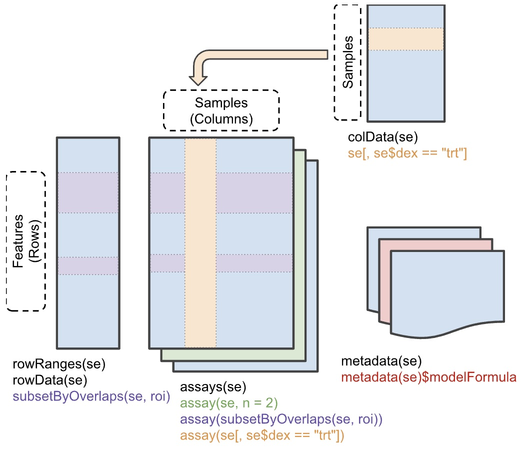
\includegraphics[width=0.8\linewidth,]{SEschema} \caption{SummarizedExperiment schematic.}\label{fig:sesc}
\end{figure}

Multiple representations of assay results may be managed in this
structure, but all assay arrays must have dimensions \(G \times N\).

For experiment collections in which the same samples are subjected
to multiple genome-scale assays, MultiAssayExperiment containers are used. See Figure \ref{fig:masc} for the layout.

\begin{figure}
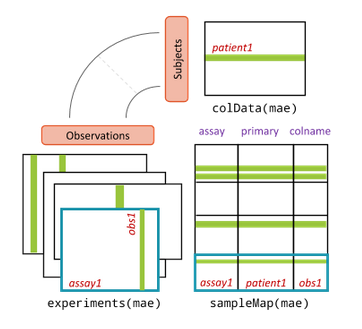
\includegraphics[width=0.8\linewidth,]{MAEschema} \caption{MultiAssayExperiment schematic.}\label{fig:masc}
\end{figure}

Further details on these data structures will be provided in section \ref{class}.

\subsection{Downloading and caching cancer genomics data and annotations}\label{cache}}

Downloading and managing data from various online resources
can be excessively time consuming. Bioconductor encourages data caching for
increased efficiency and reproducibility. The caching data methods
employed in Bioconductor
allow analysis code to
concisely refer to data resources as needed, with minimal attention to how
data are stored, retrieved or transformed.
It allows for easy management and reuse of data that are on remote
servers or in cloud, storing source
location and providing information for data updates. The BiocFileCache
Bioconductor package handles data management from within R.

BiocFileCache is a general-use caching system but Bioconductor also provides
``Hubs'', AnnotationHub and ExperimentHub, to help distributed annotation or
experimental data hosted externally. Both AnnotationHub and ExperimentHub use
BiocFileCache to handle download and caching of data.

AnnotationHub provides a centralized repository of diverse genomic annotations,
facilitating easy access and integration into analyses. Researchers can
seamlessly retrieve information such as genomic features, functional
annotations, and variant data, streamlining the annotation process for their
analyses.

ExperimentHub extends this concept to experimental data. It serves as a
centralized hub for storing and sharing curated experiment-level datasets,
allowing researchers to access a wide range of experimental designs and
conditions. This cloud-based infrastructure enhances collaboration and promotes
the reproducibility of analyses across different laboratories.

The curatedTCGAData package provides some resources through
ExperimentHub, as do many other self-identified ``CancerData'' resources. Once the
ExperimentHub is loaded, it can be queried for terms of interest.

\begin{shaded}
\begin{verbatim}
library(ExperimentHub)
eh = ExperimentHub()
query(eh, "CancerData")
## ExperimentHub with 1742 records
## # snapshotDate(): 2024-04-29
## # $dataprovider: Eli and Edythe L. Broad Institute of Harvard and MIT, GEO, ...
## # $species: Homo sapiens, Mus musculus, NA
## # $rdataclass: SummarizedExperiment, RaggedExperiment, matrix, list, DFrame,...
## # additional mcols(): taxonomyid, genome, description,
## #   coordinate_1_based, maintainer, rdatadateadded, preparerclass, tags,
## #   rdatapath, sourceurl, sourcetype 
## # retrieve records with, e.g., 'object[["EH558"]]' 
## 
##            title                                
##   EH558  | ACC_CNASNP-20160128                  
##   EH559  | ACC_CNVSNP-20160128                  
##   EH560  | ACC_colData-20160128                 
##   EH561  | ACC_GISTIC_AllByGene-20160128        
##   EH562  | ACC_GISTIC_ThresholdedByGene-20160128
##   ...      ...                                  
##   EH8533 | tcga_transcript_counts               
##   EH8534 | target_rhabdoid_wgbs_hg19            
##   EH8567 | xenium_hs_breast_addon               
##   EH9482 | Capper_example_betas.rda             
##   EH9483 | GIMiCC_Library.rda    
\end{verbatim}
\end{shaded}

%\texttt{\{r useeh\} \textless{}!-\/- , fig.cap="ExperimentHub attachment, retrieval, query, and response when seeking cancer-related data.", message=FALSE\} -\/-\textgreater{} library(ExperimentHub) eh \textless{}- ExperimentHub() query(eh, "CancerData")}

Multiple terms can be used to narrow results before choosing a download.

\begin{shaded}
\begin{verbatim}
query(eh, c("CancerData", "esophageal"))
## ExperimentHub with 2 records}
## snapshotDate(): 2023-10-24}
## $dataprovider: University of California San Francisco}
## $species: Homo sapiens}
## $rdataclass: RangedSummarizedExperiment, data.frame}
## additional mcols(): taxonomyid, genome, description,}
##   coordinate_1_based, maintainer, rdatadateadded, preparerclass, tags,}
##   rdatapath, sourceurl, sourcetype }
## retrieve records with, e.g., object[["EH8527"]]
##            title                           
##   EH8527 | cao_esophageal_wgbs_hg19        
##   EH8530 | cao_esophageal_transcript_counts
\end{verbatim}
\end{shaded}

Similarly AnnotationHub files can be downloaded for annotating data. For example,
the ensembl 110 release of gene and protein annotations are obtained with the
following:

\begin{shaded}
\begin{verbatim}
library(AnnotationHub)
ah = AnnotationHub()
query(ah, c("ensembl", "110", "Homo sapiens"))
#snapshotDate(): 2024-04-29
#AnnotationHub with 1 record
## snapshotDate(): 2024-04-29
## names(): AH113665
## $dataprovider: Ensembl
## $species: Homo sapiens
## $rdataclass: EnsDb
## $rdatadateadded: 2023-04-25
## $title: Ensembl 110 EnsDb for Homo sapiens
## $description: Gene and protein annotations for Homo sapiens based on Ensem...
## $taxonomyid: 9606
## $genome: GRCh38
## $sourcetype: ensembl
## $sourceurl: http://www.ensembl.org
## $sourcesize: NA
## $tags: c("110", "Annotation", "AnnotationHubSoftware", "Coverage",
##   "DataImport", "EnsDb", "Ensembl", "Gene", "Protein", "Sequencing",
##   "Transcript") 
## retrieve record with 'object[["AH113665"]]' 
\end{verbatim}
\end{shaded}


\section{Exploring institutionally curated cancer genomics data}\label{exploring-institutionally-curated-cancer-genomics-data}}


\subsection{The Cancer Genome Atlas}\label{the-cancer-genome-atlas}}

An overview of Bioconductor's resource for the Cancer
Genome Atlas (TCGA) is easy to obtain, with the
curatedTCGAData package.

\begin{shaded}
\begin{verbatim}
library(curatedTCGAData)
tcgatab = curatedTCGAData(version="2.1.1")
\end{verbatim}
\end{shaded}
%\begin{Shaded}
%\begin{Highlighting}[]
%\KeywordTok{library}\NormalTok{(curatedTCGAData)}
%\NormalTok{tcgatab =}\StringTok{ }\KeywordTok{curatedTCGAData}\NormalTok{(}\DataTypeTok{version=}\StringTok{"2.1.1"}\NormalTok{)}
%\end{Highlighting}
%\end{Shaded}

Records obtained for adrenocortical carcinoma (code ACC) are in Table \ref{tab:tab-lktab}.

\begin{table}

\caption{\label{tab:tab-lktab}Records returned by curatedTCGAData::curatedTCGAData(), filtered to those pertaining to adrenocortical carcinoma.}
\centering
\begin{tabular}[t]{lllll}
\toprule
  & ah\_id & title & file\_size & rdataclass\\
\midrule
1 & EH4737 & ACC\_CNASNP-20160128 & 0.8 Mb & RaggedExperiment\\
2 & EH4738 & ACC\_CNVSNP-20160128 & 0.2 Mb & RaggedExperiment\\
3 & EH4740 & ACC\_GISTIC\_AllByGene-20160128 & 0.2 Mb & SummarizedExperiment\\
4 & EH4741 & ACC\_GISTIC\_Peaks-20160128 & 0 Mb & RangedSummarizedExperiment\\
5 & EH4742 & ACC\_GISTIC\_ThresholdedByGene-20160128 & 0.2 Mb & SummarizedExperiment\\
\addlinespace
6 & EH4744 & ACC\_Methylation-20160128\_assays & 239.2 Mb & SummarizedExperiment\\
7 & EH4745 & ACC\_Methylation-20160128\_se & 6 Mb & RaggedExperiment\\
8 & EH4747 & ACC\_Mutation-20160128 & 0.7 Mb & SummarizedExperiment\\
9 & EH4748 & ACC\_RNASeq2Gene-20160128 & 2.7 Mb & SummarizedExperiment\\
10 & EH4750 & ACC\_RPPAArray-20160128 & 0.1 Mb & SummarizedExperiment\\
\addlinespace
414 & EH8118 & ACC\_miRNASeqGene-20160128 & 0.2 Mb & SummarizedExperiment\\
415 & EH8119 & ACC\_RNASeq2GeneNorm-20160128 & 5.4 Mb & SummarizedExperiment\\
\bottomrule
\end{tabular}
\end{table}

Various conventions are in play in this table. The ``title'' field is
of primary concern. The title string can be decomposed into
substrings with interpretation
\texttt{{[}tumorcode{]}\_{[}assay{]}-{[}date{]}\_{[}optional codes{]}}. The column \texttt{ah\_id} will be
explained in section \ref{hubs}, and entries in column
\texttt{rdataclass} will be discussed in section \ref{class} below.


\subsubsection{Tumor code resolution}\label{tumor-code-resolution}}

There are 33 different tumor types available in TCGA. The
decoding of tumor codes for the first ten in alphabetical order is
provided in Table \ref{tab:tab-deco}.

\begin{table}

\caption{\label{tab:tab-deco}Decoding TCGA tumor code abbreviations.}
\centering
\begin{tabular}[t]{ll}
\toprule
Code & Tumor.Type\\
\midrule
ACC & Adrenocortical Carcinoma\\
BLCA & Bladder Urothelial Carcinoma\\
BRCA & Breast Invasive Carcinoma\\
CESC & Cervical Squamous Cell Carcinoma and Endocervical Adenocarcinoma\\
CHOL & Cholangiocarcinoma\\
\addlinespace
CNTL & Controls\\
COAD & Colon Adenocarcinoma\\
DLBC & Lymphoid Neoplasm Diffuse Large B-cell Lymphoma\\
ESCA & Esophageal Carcinoma\\
FPPP & FFPE Pilot Phase II\\
\addlinespace
GBM & Glioblastoma Multiforme\\
HNSC & Head and Neck Squamous Cell Carcinoma\\
KICH & Kidney Chromophobe\\
KIRC & Kidney Renal Clear Cell Carcinoma\\
KIRP & Kidney Renal Papillary Cell Carcinoma\\
\addlinespace
LAML & Acute Myeloid Leukemia\\
LCML & Chronic Myelogenous Leukemia\\
LGG & Brain Lower Grade Glioma\\
LIHC & Liver Hepatocellular Carcinoma\\
LUAD & Lung Adenocarcinoma\\
\addlinespace
LUSC & Lung Squamous Cell Carcinoma\\
MESO & Mesothelioma\\
MISC & Miscellaneous\\
OV & Ovarian Serous Cystadenocarcinoma\\
PAAD & Pancreatic Adenocarcinoma\\
\addlinespace
PCPG & Pheochromocytoma and Paraganglioma\\
PRAD & Prostate Adenocarcinoma\\
READ & Rectum Adenocarcinoma\\
SARC & Sarcoma\\
SKCM & Skin Cutaneous Melanoma\\
\addlinespace
STAD & Stomach Adenocarcinoma\\
TGCT & Testicular Germ Cell Tumors\\
THCA & Thyroid Carcinoma\\
THYM & Thymoma\\
UCEC & Uterine Corpus Endometrial Carcinoma\\
\addlinespace
UCS & Uterine Carcinosarcoma\\
UVM & Uveal Melanoma\\
\bottomrule
\end{tabular}
\end{table}


\subsubsection{Assay codes and counts}\label{assay-codes-and-counts}}

Assays performed on tumors vary across tumor types. For assay
types shared between
breast cancer, glioblastoma, and lung adenocarcinoma (code LUAD),
the numbers of tumor and normal samples available in curatedTCGAData
are provided in Table \ref{tab:tab-doassc}.

\begin{table}

\caption{\label{tab:tab-doassc}Numbers of assays available in TCGA on tumor and normal samples,
for breast cancer, glioblastoma, and lung adenocarcinoma.}
\centering
\begin{tabular}[t]{lrrrrrr}
\toprule
  & BRCA & BRCAnormal & GBM & GBMnormal & LUAD & LUADnormal\\
\midrule
CNASNP & 1089 & 1120 & 577 & 527 & 516 & 579\\
CNVSNP & 1080 & 1119 & 577 & 527 & 516 & 579\\
GISTIC\_AllByGene & 1080 & 0 & 577 & 0 & 516 & 0\\
GISTIC\_Peaks & 1080 & 0 & 577 & 0 & 516 & 0\\
GISTIC\_ThresholdedByGene & 1080 & 0 & 577 & 0 & 516 & 0\\
\addlinespace
Mutation & 988 & 5 & 283 & 7 & 230 & 0\\
RNASeq2Gene & 1093 & 119 & 153 & 13 & 515 & 61\\
RPPAArray & 887 & 50 & 233 & 11 & 365 & 0\\
RNASeq2GeneNorm & 1093 & 119 & 153 & 13 & 515 & 61\\
Methylation\_methyl27 & 314 & 29 & 285 & 0 & 65 & 24\\
\addlinespace
Methylation\_methyl450 & 783 & 102 & 140 & 14 & 458 & 34\\
\bottomrule
\end{tabular}
\end{table}


\subsubsection{An example dataset for RNA-seq from glioblastoma multiforme}\label{an-example-dataset-for-rna-seq-from-glioblastoma-multiforme}}

We obtain normalized RNA-seq data on primary tumor samples for GBM with

%\begin{Shaded}
%\begin{Highlighting}[]
%\NormalTok{gbrna =}\StringTok{ }\KeywordTok{TCGAprimaryTumors}\NormalTok{(}\KeywordTok{curatedTCGAData}\NormalTok{(}\StringTok{"GBM"}\NormalTok{, }
%    \StringTok{"RNASeq2GeneNorm"}\NormalTok{, }\DataTypeTok{dry.run=}\OtherTok{FALSE}\NormalTok{, }\DataTypeTok{version=}\StringTok{"2.1.1"}\NormalTok{))}
%\NormalTok{gbrna}
%\CommentTok{\#\# A MultiAssayExperiment object of 1 listed}
%\CommentTok{\#\#  experiment with a user{-}defined name and respective class.}
%\CommentTok{\#\#  Containing an ExperimentList class object of length 1:}
%\CommentTok{\#\#  [1] GBM\_RNASeq2GeneNorm{-}20160128: SummarizedExperiment with 18199 rows and 153 columns}
%\CommentTok{\#\# Functionality:}
%\CommentTok{\#\#  experiments() {-} obtain the ExperimentList instance}
%\CommentTok{\#\#  colData() {-} the primary/phenotype DataFrame}
%\CommentTok{\#\#  sampleMap() {-} the sample coordination DataFrame}
%\CommentTok{\#\#  \textasciigrave{}$\textasciigrave{}, \textasciigrave{}[\textasciigrave{}, \textasciigrave{}[[\textasciigrave{} {-} extract colData columns, subset, or experiment}
%\CommentTok{\#\#  *Format() {-} convert into a long or wide DataFrame}
%\CommentTok{\#\#  assays() {-} convert ExperimentList to a SimpleList of matrices}
%\CommentTok{\#\#  exportClass() {-} save data to flat files}
%\end{Highlighting}
%\end{Shaded}

\begin{shaded}
\begin{verbatim}
gbrna = TCGAprimaryTumors(curatedTCGAData("GBM",
     "RNASeq2GeneNorm", dry.run=FALSE, version="2.1.1"))
gbrna
## A MultiAssayExperiment object of 1 listed
##experiment with a user-defined name and respective class.
##Containing an ExperimentList class object of length 1:
[1] GBM_RNASeq2GeneNorm-20160128: SummarizedExperiment with 
##        18199 rows and 153 columns
##
## Functionality:
##experiments() - obtain the ExperimentList instance
##colData() - the primary/phenotype DataFrame
##sampleMap() - the sample coordination DataFrame
##`$`, `[`, `[[` - extract colData columns, subset, or experiment
####*Format() - convert into a long or wide DataFrame
assays() - convert ExperimentList to a SimpleList of matrices
##exportClass() - save data to flat files
\end{verbatim}
\end{shaded}

R functions defined in Bioconductor packages can operate on the variable \texttt{gbrna} to
retrieve information of interest. Details on the underlying data structure
are given in section \ref{class} below. For most assay types, we think of the quantitative
assay
information as tabular in nature, with table rows corresponding to genomic
features such as genes, and table columns corresponding to samples.

Information on GBM samples employs the \texttt{colData} function.

%\begin{shaded}
%\begin{Highlighting}[]
%\KeywordTok{dim}\NormalTok{(}\KeywordTok{colData}\NormalTok{(gbrna))}
%\CommentTok{\#\# [1]  153 4380}
%\end{Highlighting}
%\end{shaded}


\begin{shaded}
\begin{verbatim}
dim(colData(gbrna))
## [1] 153 4380
\end{verbatim}
\end{shaded}

For sample level information obtained \texttt{colData}, we think of rows
as samples, and columns as sample attributes.


\subsubsection{Clinical and phenotypic data}
\label{clinical-and-phenotypic-data}}

TCGA datasets are generally provided as combinations of
results for tumor tissue and normal tissue. The determination
of a record's sample type is encoded in the sample ``barcode''.
Decoding of sample barcodes is described at 

\begin{verbatim}
https://docs.gdc.cancer.gov/Encyclopedia/pages/TCGA_Barcode/
\end{verbatim}

\noindent
with specific interpretation of sample types listed 
at
{\small
\begin{verbatim}
https://gdc.cancer.gov/resources-tcga-users/tcga-code-tables/sample-type-codes
\end{verbatim}
}
\noindent
separately. The TCGAutils package provides utilities for extracting
data on primary tumor samples, excluding samples that may have been taken on
normal tissue or metastases.

Clinical and phenotypic data on all TCGA samples are voluminous. For example,
there are 2684 fields of sample level data for BRCA
samples, and 4380 fields for GBM samples. Many of these
fields are meaningfully populated for only a very small minority of samples.
To see this for GBM:

%\begin{shaded}
%\begin{Highlighting}[]
%\KeywordTok{mean}\NormalTok{(}\KeywordTok{sapply}\NormalTok{(}\KeywordTok{colData}\NormalTok{(gbrna), }\ControlFlowTok{function}\NormalTok{(x) }\KeywordTok{mean}\NormalTok{(}\KeywordTok{is.na}\NormalTok{(x))}\OperatorTok{\textgreater{}}\NormalTok{.}\DecValTok{90}\NormalTok{))}
%\CommentTok{\#\# [1] 0.8091324}
%\end{Highlighting}
%\end{shaded}

\begin{shaded}
\begin{verbatim}
mean(sapply(colData(gbrna), function(x) mean(is.na(x))>.90))
## [1] 0.8091324
\end{verbatim}
\end{shaded}

In words, for 81\% of clinical data fields in TCGA GBM data,
at least 90\% of entries are missing.

Nevertheless, with careful inspection of fields and contents,
nearly complete clinical data can be extracted and combined with molecular
and genetic assay data with modest effort.

The following code chunk illustrates a very crude
approach to comparing survival profiles for BRCA, GBM, and LUAD
donors. The result is in Figure \ref{fig:dothesurv}.


{\small
\begin{shaded}
\begin{verbatim}
# obtain mutation data for BRCA, GBM, LUAD; could use any or all assay types
brmut = curatedTCGAData("BRCA", "Mutation", version = "2.1.1", dry.run = FALSE)
gbmut = curatedTCGAData("GBM", "Mutation", version = "2.1.1", dry.run = FALSE)
lumut = curatedTCGAData("LUAD", "Mutation", version = "2.1.1", dry.run = FALSE)
# extract survival times
library(survival)
getSurv = function(mae) {
 days_on = with(colData(mae), ifelse(is.na(days_to_last_followup),
 days_to_death, days_to_last_followup))
 Surv(days_on, colData(mae)$vital_status)
}
ss = lapply(list(brmut, gbmut, lumut), getSurv)
codes = c("BRCA", "GBM", "LUAD")
type = factor(rep(codes, sapply(ss,length)))
allsurv = do.call(c, ss)
library(GGally)
ggsurv(survfit(allsurv~type))
\end{verbatim}
\end{shaded}
}

\begin{figure}
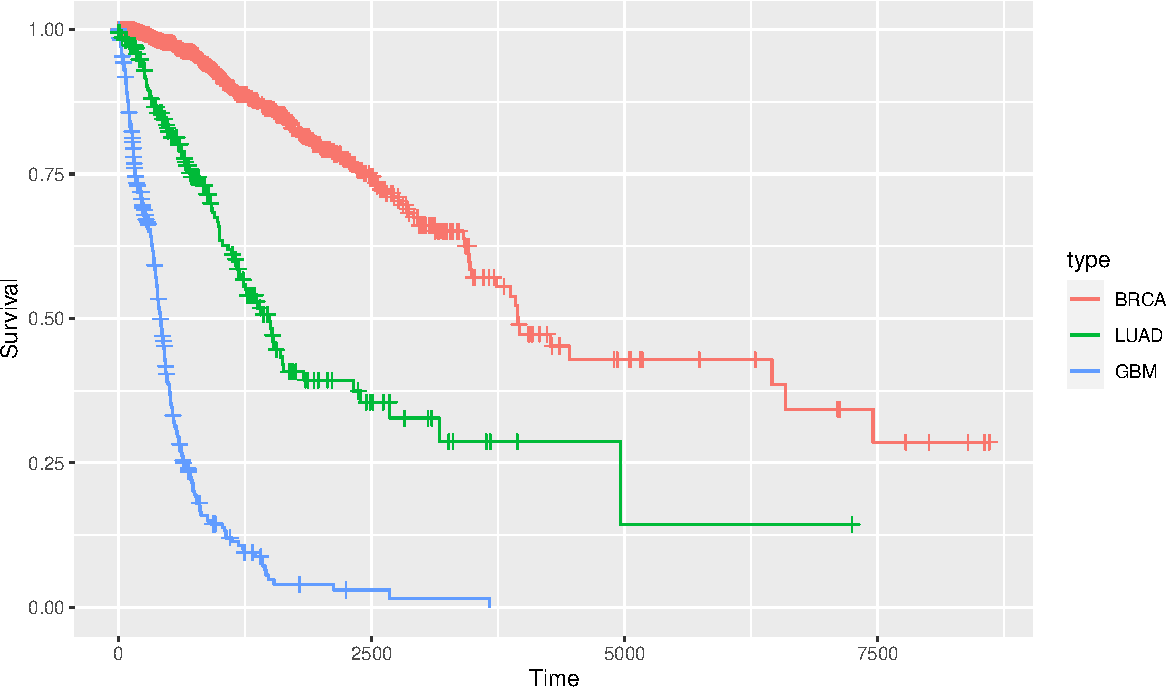
\includegraphics[width=0.8\linewidth,]{bioccb_files/figure-latex/dothesurv-1} \caption{Survival profile extraction from three MultiAssayExperiments produced with curatedTCGAData calls.}\label{fig:dothesurv}
\end{figure}

At this point, survival times within tumor type can be stratified by any
features of the mutation profiles of individual samples.
The ``RaggedExperiment'' class is employed to test each BRCA sample for
presence of any mutation in the gene TTN. See Figure \ref{fig:strat}.

\begin{shaded}
\begin{verbatim}
bprim = TCGAprimaryTumors(brmut)
## harmonizing input:
## removing 5 sampleMap rows with 'colname' not in 
##      colnames of experiments
mutsyms = assay(experiments(bprim)[[1]], "Hugo_Symbol")
cn = rownames(colData(bprim)) # short
cna = colnames(mutsyms) # long
cnas = substr(cna, 1, 12)
hasTTNmut = apply(assay(experiments(TCGAprimaryTumors(brmut))[[1]], 
     "Hugo_Symbol"), 2, function(x) length(which(x=="TTN"))>0)
## harmonizing input:
## removing 5 sampleMap rows with 'colname' not in
##      colnames of experiments
names(hasTTNmut) = cnas
bsurv = getSurv(TCGAprimaryTumors(brmut))
## harmonizing input:
## removing 5 sampleMap rows with 'colname' not in 
##      colnames of experiments
hasTTNmut = hasTTNmut[cn] # match mutation records to surv times
ggsurv(survfit(bsurv~hasTTNmut))
\end{verbatim}
\end{shaded}


\begin{figure}
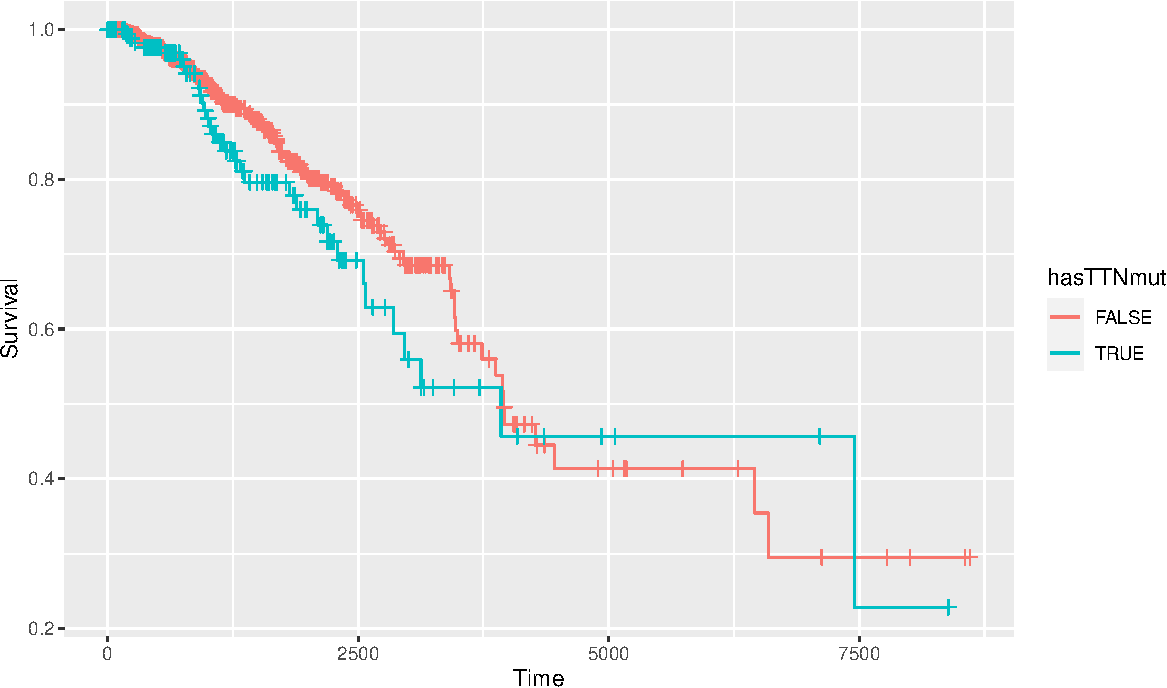
\includegraphics[width=1\linewidth,]{bioccb_files/figure-latex/strat-1} \caption{Survival distributions for donors of breast tumors in TCGA, stratified by presence or absence of mutation in gene TTN.}\label{fig:strat}
\end{figure}

Similar manipulations permit exploration of relationships between
any molecular assay outcomes and any clinical data collected in TCGA.


\subsection{cBioPortal}\label{cbioportal}}

The cBioPortal user guide
at 
\begin{verbatim}
https://www.cbioportal.org/
\end{verbatim}
defines the goal of the portal to be reducing ``the barriers between complex
genomic data and cancer researchers by providing rapid, intuitive, and high-quality
access to molecular profiles and clinical attributes from large-scale cancer genomics projects, and
therefore to empower researchers to translate these rich data sets into biologic insights and clinical applications.''

Bioconductor's cBioPortalData package simplifies access to over 300 genomic studies of
diverse cancers in cBioPortal. The main unit of data access is the publication. The
\texttt{cBioPortal} function mediates a connection between an R session and the
cBioPortal API. \texttt{getStudies} returns a tibble with metadata on
all studies.

\begin{shaded}
\begin{verbatim}
library(cBioPortalData)
cbio = cBioPortal()
allst = getStudies(cbio)
dim(allst)
## [1] 397 13
\end{verbatim}
\end{shaded}

A pruned selection of records from the cBioPortal
studies table is given in Table \ref{tab:tab-cball}.

\begin{table}
\caption{\label{tab:tab-cball}Excerpts from four fields on selected records in the cBioPortal getStudies output.}\\
\begin{tabular}{p{5cm}p{5cm}l}
name & description & studyId \\ \hline
Adenoid Cystic Carcinoma of the Breast & Whole exome sequencing of 12 breast AdCCs. & acbc\_mskcc\_2015 \\
Adenoid Cystic Carcinoma & Whole-exome or whole-genome sequencing analysis of 60 ACC tumor/normal pairs & acyc\_mskcc\_2013 \\
Adenoid Cystic Carcinoma & Targeted Sequencing of 28 metastatic Adenoid Cystic Carcinoma samples. & acyc\_fmi\_2014 \\
Adenoid Cystic Carcinoma & Whole-genome or whole-exome sequencing of 25 adenoid cystic carcinoma tumor/normal pairs. & acyc\_jhu\_2016 \\
Adenoid Cystic Carcinoma & WGS of 21 salivary ACCs and targeted molecular analyses of a validation set (81 patients). & acyc\_mda\_2015 \\
Adenoid Cystic Carcinoma & Whole-genome/exome sequencing of 10 ACC PDX models. & acyc\_mgh\_2016 \\
Adenoid Cystic Carcinoma & Whole exome sequencing of 24 ACCs. & acyc\_sanger\_2013 \\
Adenoid Cystic Carcinoma Project & Multi-Institute Cohort of 1045 Adenoid Cystic Carcinoma patients. & acc\_2019 \\
Basal Cell Carcinoma & Whole-exome sequencing of 126 basal cell carcinoma tumor/normal pairs; targeted sequencing of 163 sporadic samples (40 tumor/normal pairs) and 4 Gorlin symdrome basal cell carcinomas. & bcc\_unige\_2016 \\
\end{tabular}
\end{table}

%\begin{table}[lll]%{>{\raggedright\arraybackslash}p{12em}>{\raggedright\arraybackslash}p{15em}l}
%\caption{\label{tab:tab-cball}Excerpts from four fields on selected records in the cBioPortal getStudies output.}\\
%\toprule
%name & description & studyId\\
%\midrule
%Adenoid Cystic Carcinoma of the Breast & Whole exome sequencing of 12 breast AdCCs. & acbc\_mskcc\_2015\\
%Adenoid Cystic Carcinoma & Whole-exome or whole-genome sequencing analysis of 60 ACC tumor/normal pairs & acyc\_mskcc\_2013\\
%Adenoid Cystic Carcinoma & Targeted Sequencing of 28 metastatic Adenoid Cystic Carcinoma samples. & acyc\_fmi\_2014\\
%Adenoid Cystic Carcinoma & Whole-genome or whole-exome sequencing of 25 adenoid cystic carcinoma tumor/normal pairs. & acyc\_jhu\_2016\\
%Adenoid Cystic Carcinoma & WGS of 21 salivary ACCs and targeted molecular analyses of a validation set (81 patients). & acyc\_mda\_2015\\
%\addlinespace
%Adenoid Cystic Carcinoma & Whole-genome/exome sequencing of 10 ACC PDX models. & acyc\_mgh\_2016\\
%Adenoid Cystic Carcinoma & Whole exome sequencing of 24 ACCs. & acyc\_sanger\_2013\\
%Adenoid Cystic Carcinoma Project & Multi-Institute Cohort of 1045 Adenoid Cystic Carcinoma patients. & acc\_2019\\
%Basal Cell Carcinoma & Whole-exome sequencing of 126 basal cell carcinoma tumor/normal pairs; targeted sequencing of 163 sporadic samples (40 tumor/normal pairs) and 4 Gorlin symdrome basal cell carcinomas. & bcc\_unige\_2016\\
%\bottomrule
%\end{table}

To explore copy number alteration data from a study on angiosarcoma,
we find the associated studyId field in \texttt{allst} and use the \texttt{cBioDataPack} function
to retrieve a MultiAssayExperiment:

\begin{shaded}
\begin{verbatim}
ann = "angs_project_painter_2018"
ang = cBioDataPack(ann)
ang
## A MultiAssayExperiment object of 3 listed
##experiments with user-defined names and respective classes.
####Containing an ExperimentList class object of length 3:
##[1] cna_hg19.seg: RaggedExperiment with 27835 rows and 48 columns
##[2] cna: SummarizedExperiment with 23109 rows and 48 columns
##[3] mutations: RaggedExperiment with 24058 rows and 48 columns
## Functionality:
##experiments() - obtain the ExperimentList instance
##colData() - the primary/phenotype DataFrame
##sampleMap() - the sample coordination DataFrame
##`$`, `[`, `[[` - extract colData columns, subset, or experiment
####*Format() - convert into a long or wide DataFrame
assays() - convert ExperimentList to a SimpleList of matrices
##exportClass() - save data to flat files
\end{verbatim}
\end{shaded}

The copy number alteration outcomes are in the
\texttt{assay} component of the experiment.

\begin{shaded}
\begin{verbatim}
seg = experiments(ang)[[1]]
colnames(seg) = sapply(strsplit(colnames(seg), "-"), "[", 5)
assay(seg)[1:4,1:4]
##
##                   DAE1F DACME DADBW DAD34
## 1:12227-955755       71    NA    NA    NA
## 1:957844-1139868     62    NA    NA    NA
## 1:1140874-1471177   167    NA    NA    NA
## 1:1475170-1855370   113    NA    NA    NA
\end{verbatim}
\end{shaded}

The rownames component of this matrix can be transformed to
a GenomicRanges instance for concise manipulation.

\begin{shaded}
\begin{verbatim}
allalt = GRanges(rownames(assay(seg)))
 allalt
## GRanges object with 27835 ranges and 0 metadata columns:
##           seqnames            ranges strand
##              <Rle>         <IRanges>  <Rle>
##       [1]        1      12227-955755      *
##       [2]        1    957844-1139868      *
##       [3]        1   1140874-1471177      *
##       [4]        1   1475170-1855370      *
##       [5]        1  1857786-17257894      *
##       ...      ...               ...    ...
##   [27831]       20     68410-1559342      *
##   [27832]       20   1585705-1592359      *
##   [27833]       20  1616247-62904955      *
##   [27834]       21  9907492-48084286      *
##   [27835]       22 16157938-51237572      *
##   -------
##   seqinfo: 22 sequences from an unspecified genome; no seqlengths
\end{verbatim}
\end{shaded}


We'll focus on chromosome 17, where TP53 is found. Regions
of genomic alteration are summarized to their midpoints.
The display in Figure \ref{fig:mkden} shows a strong peak in the vicinity of 7.5 Mb on chromosome 17, near TP53.

\begin{shaded}
\begin{verbatim}
g17 = allalt[seqnames(allalt)=="17"]
df17 = as(g17, "data.frame")
df17$mid = .5*(df17$start+df17$end) # midpoint only
ggplot(df17, aes(x=mid)) + geom_density(bw=.2) + xlab("chr 17 bp")
\end{verbatim}
\end{shaded}


\begin{figure}
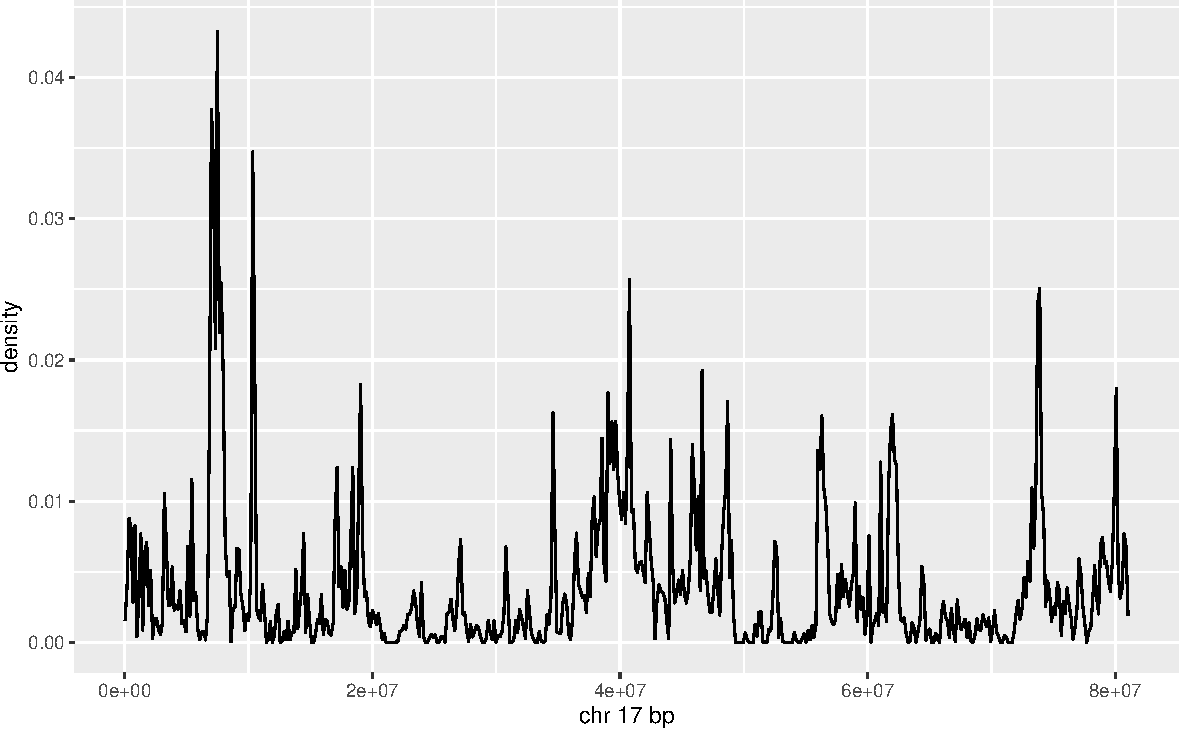
\includegraphics[width=1\linewidth,]{bioccb_files/figure-latex/mkden-1} \caption{Density of recurrent genomic alterations on chromosome 17 for 48 angiosarcoma patients.}\label{fig:mkden}
\end{figure}



\section{Genomic annotation resources relevant to cancer}\label{hubs}


\subsection{Resources from UCSC, NCBI, and EMBL}\label{resources-from-ucsc-ncbi-and-embl}

Sequences for reference genome builds for human and
other model organisms are supplied in BSgenome packages.
BSgenome.Hsapiens.UCSC.hg19 provides all chromosomes and
contigs for the 2009 build; the hg38 suffix may be used
for the 2013 build. The recent ``telomere to telomere''
build is available as BSgenome.Hsapiens.NCBI.T2T.CHMv13v2.0.

NCBI's dbSNP catalog of genetic variants is provided
in versioned packages.
For example, SNPlocs.Hsapiens.dbSNP155.GRCh38 includes
position and nucleotide content information for over
1 billion SNP identifiers ("rs numbers").

Tracks defined for the UCSC genome browser are also
packaged. The package 
\begin{verbatim}
TxDb.Hsapiens.UCSC.knownGene.hg38 
\end{verbatim} 
can be
used to get gene, transcript, and exon location information
for the hg38 build. The EnsDb packages provide similar
information for annotations curated at EMBL.

%\begin{shaded}
%\KeywordTok{library}\NormalTok{(EnsDb.Hsapiens.v86)}
%\NormalTok{EnsDb.Hsapiens.v86}
%\CommentTok{\#\# EnsDb for Ensembl:}
%\CommentTok{\#\# |Backend: SQLite}
%\CommentTok{\#\# |Db type: EnsDb}
%\CommentTok{\#\# |Type of Gene ID: Ensembl Gene ID}
%\CommentTok{\#\# |Supporting package: ensembldb}
%\CommentTok{\#\# |Db created by: ensembldb package from Bioconductor}
%\CommentTok{\#\# |script\_version: 0.3.0}
%\CommentTok{\#\# |Creation time: Thu May 18 16:32:27 2017}
%\CommentTok{\#\# |ensembl\_version: 86}
%\CommentTok{\#\# |ensembl\_host: localhost}
%\CommentTok{\#\# |Organism: homo\_sapiens}
%\CommentTok{\#\# |taxonomy\_id: 9606}
%\CommentTok{\#\# |genome\_build: GRCh38}
%\CommentTok{\#\# |DBSCHEMAVERSION: 2.0}
%\CommentTok{\#\# | No. of genes: 63970.}
%\CommentTok{\#\# | No. of transcripts: 216741.}
%\CommentTok{\#\# |Protein data available.}
%\end{Highlighting}
%\end{shaded}

\begin{shaded}
\begin{verbatim}
library(EnsDb.Hsapiens.v86)
EnsDb.Hsapiens.v86
## EnsDb for Ensembl:
## |Backend: SQLite
## |Db type: EnsDb
## |Type of Gene ID: Ensembl Gene ID
## |Supporting package: ensembldb
## |Db created by: ensembldb package from Bioconductor
## |script\_version: 0.3.0
## |Creation time: Thu May 18 16:32:27 2017
## |ensembl\_version: 86
## |ensembl\_host: localhost
## |Organism: homo\_sapiens
## |taxonomy\_id: 9606
## |genome\_build: GRCh38
## |DBSCHEMAVERSION: 2.0
## | No. of genes: 63970.
## | No. of transcripts: 216741.
## |Protein data available.
\end{verbatim}
\end{shaded}


The ``genes'' method provides addresses and additional
annotations.

\begin{shaded}
\begin{verbatim}
names(mcols(genes(EnsDb.Hsapiens.v86)))
## [1] "gene_id"          "gene_name"        "gene_biotype"     
## [4] "seq_coord_system" "symbol"           "entrezid"
head(table(genes(EnsDb.Hsapiens.v86)$gene_biotype))
##      3prime_overlapping_ncRNA                     antisense 
##                            30                          5703 
## bidirectional_promoter_lncRNA                     IG_C_gene 
##                             4                            23 
##               IG_C_pseudogene                     IG_D_gene 
##                            11                            64
\end{verbatim}
\end{shaded}

More recent versions of Ensembl gene annotation are available
from AnnotationHub, as illustrated above in section \ref{cache} with
the creation of \texttt{ens110}.

\subsection{Gene sets}\label{gene-sets}

Many methods have been developed to employ collections
of genes for inference on hypotheses about cancer
initiation or progression. The Molecular Signatures Database (MSigDB)
is curated at Broad Institute, and can be harvested
using the msigdb package.

Collect all gene sets for humans:

\begin{shaded}
\begin{verbatim}
library(msigdb)
hssigs = getMsigdb(org="hs", id="SYM", version=getMsigdbVersions())
\end{verbatim}
\end{shaded}

Find those with CANCER in their name:

\begin{shaded}
\begin{verbatim}
nms = grep("CANCER", names(hssigs), value=TRUE)
head(nms)
## [1] "SOGA_COLORECTAL_CANCER_MYC_DN"
## [2] "SOGA_COLORECTAL_CANCER_MYC_UP"
## [3] "WATANABE_RECTAL_CANCER_RADIOTHERAPY_RESPONSIVE_UP"
## [4] "LIU_PROSTATE_CANCER_UP"
## [5] "BERTUCCI_MEDULLARY_VS_DUCTAL_BREAST_CANCER_UP"
## [6] "WATANABE_COLON_CANCER_MSI_VS_MSS_UP"
wangmet = hssigs[["WANG_METASTASIS_OF_BREAST_CANCER_ESR1_UP"]]
wangmet
## setName: WANG_METASTASIS_OF_BREAST_CANCER_ESR1_UP
## geneIds: KPNA2, HDGFL3, ..., PSMC2 (total: 22)
## geneIdType: Symbol
## collectionType: Broad
##bcCategory: c2 (Curated)
##bcSubCategory: CGP
## details: use 'details(object)'
\end{verbatim}
\end{shaded}

Information on provenance is bound together with the gene list:

\begin{shaded}
\begin{verbatim}
details(wangmet)
## setName: WANG_METASTASIS_OF_BREAST_CANCER_ESR1_UP
## geneIds: KPNA2, HDGFL3, ..., PSMC2 (total: 22)
## geneIdType: Symbol
## collectionType: Broad
##bcCategory: c2 (Curated)
##bcSubCategory: CGP
## setIdentifier: LVY1HGGWMJ7:35020:Fri May 26 13:33:02 2023:1104005
## description: Genes whose expression in primary ER(+) 
##      [GeneID=2099] breast cancer tumors positively correla
## (longDescription available)
## organism: Homo sapiens
## pubMedIds: 15721472
## urls: https://data.broadinstitute.org/gsea-msigdb/msigdb/
##    release/2023.1.Hs/msigdb_v2023.1.Hs.xml.zip
## contributor: Arthur Liberzon
\end{verbatim}
\end{shaded}

\subsection{Ontologies}\label{ontologies}

Informal reasoning about cancer genomics employs conventional
but frequently ambiguous terminology. In modern
information science, ontologies are structured vocabularies
(sets of ``terms'', which may be single words or natural language
phrases) accompanied by
explicit statements of semantic relationships among terms.

Bioconductor provides several approaches for using ontologies
in cancer data science. The most familiar ontology
in this domain is Gene Ontology (GO), which organizes vocabulary
about genes and gene products in
the areas of molecular function, cellular components, and
biological processes.

\subsubsection{Ontology usage with AnnotationDbi}\label{ontology-usage-with-annotationdbi}

A common use case is to find genes or proteins associated
with some biological process, component, or function.
A phrase like `Golgi membrane' can be found in Gene Ontology
using the select method with GO.db:

\begin{shaded}
\begin{verbatim}
library(GO.db)
select(GO.db, keytype="TERM",
keys="Golgi membrane", columns=c("GOID", "DEFINITION", "ONTOLOGY"))
##             TERM       GOID
## 1 Golgi membrane GO:0000139
##                                 DEFINITION
## 1 The lipid bilayer surrounding any of the 
## compartments of the Golgi apparatus.
## ONTOLOGY
## 1     CC
\end{verbatim}
\end{shaded}

Once the formal identifier is obtained, the org.Hs.eg.db package can be used to find mappings
from the GO term to gene and protein identifiers. This generates a fairly large table:

\begin{shaded}
\begin{verbatim}
library(org.Hs.eg.db)
go139 = select(org.Hs.eg.db, keys="GO:0000139", keytype="GO",
columns=c("ENTREZID", "SYMBOL", "PFAM"))
dim(go139)
## [1] 1212 6
head(go139)
##           GO EVIDENCE ONTOLOGY ENTREZID SYMBOL    PFAM
## 1 GO:0000139      TAS       CC       28    ABO PF03414
## 2 GO:0000139      IEA       CC      102 ADAM10 PF00200
## 3 GO:0000139      IEA       CC      102 ADAM10 PF13574
## 4 GO:0000139      IEA       CC      102 ADAM10 PF01562
## 5 GO:0000139      TAS       CC      162  AP1B1 PF09066
## 6 GO:0000139      TAS       CC      162  AP1B1 PF01602
\end{verbatim}
\end{shaded}

The evidence code TAS means that there is a ``traceable author statement'' associating the term
of interest with the gene identified. The number of genes in traceable Golgi membrane:gene
associations is found with

\begin{shaded}
\begin{verbatim}
go139 |> dplyr::filter(EVIDENCE=="TAS") |> distinct(ENTREZID) |> count()
##       n
## [1] 327
\end{verbatim}
\end{shaded}


\subsubsection{Ontology usage with rols}\label{ontology-usage-with-rols}

Access to a vast collection of ontologies is afforded by the EBI's
Ontology Lookup Service (OLS). The rols package uses the OLS API
to discover ontologic mapping of terms of interest. Here we'll
consider the term ``golgi membrane dynamics'', which is not found in GO.
Again a multistep process is used.

\begin{shaded}
\begin{verbatim}
library(rols)
lk1 = OlsSearch(q="golgi membrane dynamics", exact=TRUE)
lk1
## Object of class 'OlsSearch':
##query: golgi membrane dynamics
##requested: 20 (out of 3)
##response(s): 0
\end{verbatim}
\end{shaded}


In this first step, we find how extensive is the response
to the query. Certain searches yield tens of thousands of hits.
With the exact parameter setting, the yield is modest.
Now we extract a data.frame after requesting all
records with \texttt{olsSearch}.  Results are
excerpted in Table \ref{tab:tab-golg}.

\begin{shaded}
\begin{verbatim}
lk2 = olsSearch(lk1)
lk3 = as(lk2, "data.frame")
lk3$description = unlist(lk3$description)
\end{verbatim}
\end{shaded}



\begin{table}
\caption{Using rols to obtain ontologic information related to
golgi membrane dynamics. \label{tab:tab-golg}}
\begin{tabular}{lp{5cm}p{8cm}}
\toprule
short\_form & description & label\\
\midrule
NCIT\_C119637 & This gene is involved in both protein ubiquitination and Golgi membrane dynamics. & HACE1 Gene\\
NCIT\_C119639 & E3 ubiquitin-protein ligase HACE1 (909 aa, \textasciitilde{}102 kDa) is encoded by the human HACE1 gene. This protein is involved in the regulation of both the ubiquitination and subsequent degradation of small GTPases, which modulates Golgi membrane dynamics. & E3 Ubiquitin-Protein Ligase HACE1\\
NCIT\_C119638 & Human HACE1 wild-type allele is located in the vicinity of 6q16.3 and is approximately 132 kb in length. This allele, which encodes E3 ubiquitin-protein ligase HACE1 protein, plays a role in the modulation of both Golgi membrane dynamics and ubiquitination. Mutations of the gene, including translocations that either reduce expression of the gene (t(6;15)(q21;q21)) or truncate the gene (t(5;6)(q21;q21)), are associated with Wilms tumor. & HACE1 wt Allele\\
\bottomrule
\end{tabular}
\end{table}

The detailed descriptions of the NCI Thesaurus entries show
the exact nature of the search outcome.

\subsubsection{Cross-ontology relationships}\label{cross-ontology-relationships}

Philosophically, ontology is the study of what there is. For
applications in information
science,
boundaries need to be established so that ontological
resources can be managed with well-defined scopes. In Gene
Ontology, three sub-ontologies are explicitly identified for
cellular components, biological processes, and molecular functions.

As knowledge of cell biology increases, the typology of
cells becomes more and more intricate. Differentiation
and definition
of ``cell types'' involves concepts from immunology,
protein science, anatomy, and other conceptual domains
for which ontologies have been developed. Figure \ref{fig:ontopair}
presents, on the left, the hierarchy of cell type concepts starting at ``lymphocyte'',
leading to ``Type II Natural Killer T cell secreting interferon gamma''.
On the right, some of the GO and Protein Ontology (PR) cross-references
in the Cell Ontology (CL) entry for the Type II NK cell are shown.
The ``cond'' column of the table contains abbreviated tokens
representing formal relationships linking the cell type
to the protein or cellular component elements of PR and GO.
The token ``hasPMP'' refers to the element of the Relation Ontology
(RO) ``has plasma membrane part'' (RO:0002104).

\begin{figure}
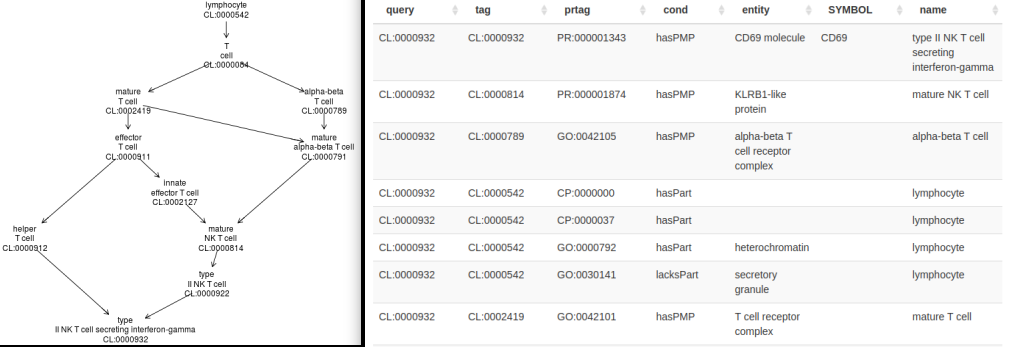
\includegraphics[width=1\linewidth,]{ontoPair} \caption{Ontology visualization and tabulation with ontoProc::ctmarks.}\label{fig:ontopair}
\end{figure}

Prospects for use of ontological discipline in the
definition of new cell types are reviewed in a 2018
paper from the Venter Institute \cite{Aevermann2018}.

The field of biological ontology is rapidly advancing,
and the integration of ontology search and inference
with data analytic frameworks requires more effort at this time.




\section{Analytical workflows}\label{analytical-workflows}


\subsection{Overview}\label{overview}

Table \ref{tab:tab-wflow} presents an informal topical
labeling for Bioconductor software packages with
cancer mentioned in the Description field of package
metadata.

\begin{table}
\caption{\label{tab:tab-wflow}Topical organization of packages with cancer applications.}
\begin{tabular}{l{4cm}p{6cm}}
\toprule
topic & packages\\
\midrule
Ancestry & RAIDS\\
Biomarkers & INDEED, iPath, RLassoCox\\
ceRNA & GDCRNATools\\
Clonal Evolution & CIMICE, LACE, OncoSimulR, TRONCO, CancerInSilico, cellscape\\
CNV & oncoscanR, SCOPE, ZygosityPredictor\\
\addlinespace
DrugSensitivity & DepInfeR, octad, PharmacoGx, rcellminer\\
Epigenetics & MethylMix, AMARETTO, COCOA, methylclock, missMethyl\\
HotSpots/Drivers/signatures & compSPOT, MoonlightR, Moonlight2R, \\
 & DriverNet, genefu, mastR, pathifier, RESOLVE, macat, \\
 & SigCheck, signeR, signifinder, supersigs, decompTumor2Sig, YAPSA\\
ImmuneModulation & easier\\
IsoformSwitching & IsoformSwitchAnalyzeR\\
\addlinespace
Literature mining & OncoScore\\
ncRNA & NoRCE\\
Radiomics & RadioGx\\
RecurrentFusion & copa, oppar\\
Spatial & SpatialDecon\\
\addlinespace
SpecificCancers & consensusOV, PDATK, STROMA4\\
Splicing & OutSplice, psichomics\\
Subtyping & SCFA\\
\end{tabular}
\bottomrule
\end{table}

The vignettes of each of these packages provide background and
illustration of their roles in cancer genomics.

\subsection{Packages supporting epigenomic analysis}\label{packages-supporting-epigenomic-analysis}

Bioconductor also provides a diverse array of packages for analysis of epigenome
data. Cancer is often studied under a developmental lens, so increasingly, studies
are measuring cell states using epigenomic methods. Epigenomics is the study of
chemical modifications and chromosomal conformations of DNA in a nucleus; in cancer
epigenomics, we study how the cancer epigenome differs among cancers and how
these relate to healthy epigenomes. As of 2023, Bioconductor includes 89 packages
under \emph{Epigenetics} and 93 packages tagged under \emph{FunctionalGenomics}, including dozens of tools
for analyzing a variety of epigenome assays, such as ATAC-seq, ChIP-seq, or
bisulfite-seq. Among these are also tools that handle more general analysis, such
as genomic region set enrichment.

First, for ATAC-seq data, bioconductor packages include general-purpose pipelines, including scPipe
\cite{Tian2018}. %(Tian et al. \protect\hyperlink{ref-Tian2018}{2018})
and esATAC \cite{Wei2018} %(Wei et al. \protect\hyperlink{ref-Wei2018}{2018}), 
which start from FASTQ files and produce feature count
matrices. Alternatively, many practitioners elect to do general-purpose pipeline processing outside of
R, and then bring the processed data into R for statistical analysis,
visualization, and quality control. In this approach, ATACseqQC
provides
a variety of QC plots specific to ATAC-seq data \cite{Ou2018}.% (Ou et al. \protect\hyperlink{ref-Ou2018}{2018}).

For DNA methylation, many popular packages have been developed to help with
all stages of a DNA methylation analysis. These include minfi 
\cite{Aryee2014}
which specializes in methylation array analysis, biseq and bsseq \cite{Hansen2012}  %(Hansen, Irizarry, and Wu \protect\hyperlink{ref-Hansen2012}{2012})
which provide fundamental infrastructure for sequencing-based assays, and RnBeads
\cite{Mueller2019},
%(Müller et al. \protect\hyperlink{ref-Mueller2019}{2019}), 
which provides a comprehensive general-purpose analysis of DNA
methylation cohorts from arrays or sequencing-based assays. Other packages provide more specialized
analysis approaches, such as MIRA \cite{Lawson2018}, %(Lawson et al. \protect\hyperlink{ref-Lawson2018}{2018}), 
which infers regulatory
activity of transcription factors using DNA methylation signals, %(Sheffield et al.~2018), FIXME not found
or ELMER, which uses DNA methylation and gene expression in large cancer
cohorts to infer transcription factor networks \cite{Silva2019}. % (Silva et al. \protect\hyperlink{ref-Silva2019}{2018}). 
EpiDISH infers
the proportions of cell-types present in a bulk sample on the basis
of DNA methylation data \cite{Zheng2018a}. %(Zheng et al. \protect\hyperlink{ref-Zheng2018a}{2018}).

%Another popular epigenome experiment is ChIP-seq, and Bioconductor delivers many packages in
%this area. 
DiffBind \cite{Stark2011} %(Stark and Brown \protect\hyperlink{ref-Stark2011}{2011}) is a popular approach for
facilitates differential binding analysis of ChIP-seq peak data.

%A variety of packages are also geared toward visualization of this type
%of data. 
GenomicDistributions \cite{Kupkova2022} % (Kupkova et al. \protect\hyperlink{ref-Kupkova2022}{2022}) 
provides a variety of plots for visualization
distributions of any type of genomic range data. The chromPlot package specializes
in plots across chromosomes.  Several packages deal with
unsupervised exploration of variation in epigenomic data. PathwayPCA, MOFA2 \cite{Argelaguet2020} %(Argelaguet et al. \protect\hyperlink{ref-Argelaguet2020}{2020})
and COCOA \cite{Lawson2020} %(Lawson et al. \protect\hyperlink{ref-Lawson2020}{2020}) 
can process any epigenomic signal data.
A variety of alternative approaches for enrichment analysis, which include LOLA \cite{Sheffield2016}, %(Sheffield and Bock \protect\hyperlink{ref-Sheffield2016}{2016}),
chipenrich, regionR \cite{Gel2015}, %(Gel et al. \protect\hyperlink{ref-Gel2015}{2015}), 
and FGNet \cite{Aibar2015}. %(Aibar et al. \protect\hyperlink{ref-Aibar2015}{2015}).
Annotation packages include ChIPpeakAnno \cite{Zhu2010} % (Zhu et al. \protect\hyperlink{ref-Zhu2010}{2010})
and annotatr \cite{Cavalcante2017}.%(Cavalcante and Sartor \protect\hyperlink{ref-Cavalcante2017}{2017}) are popular packages for annotating genomic
%ranges.


\subsection{Some details on prediction of responsiveness to immune checkpoint blockade}\label{some-details-on-prediction-of-responsiveness-to-immune-checkpoint-blockade}

The National Cancer Institute website on checkpoint inhibitors
in cancer immunotherapy (``Immune Checkpoint Inhibitors'' 
\cite{ICBnci}) %\protect\hyperlink{ref-ICBnci}{2022})
lists 12 different cancer types
amenable to treatment via immune checkpoint inhibition.
The ``easier'' package in Bioconductor
assembles multiple systems biology resources
to produce patient-specific
prediction of responsiveness to
immune checkpoint blockade (ICB) \cite{easierPap}. %, as described in Lapuente-Santana et al. (\protect\hyperlink{ref-easierPap}{2021}).

Figure \ref{fig:easfin} presents on overview of results of
immune response assessment in a cohort of patients with
bladder cancer \cite{Mariathasan2018}. %reported in Mariathasan et al. (\protect\hyperlink{ref-Mariathasan2018}{2018}).
Patient's bulk RNA-seq data are used to develop multiple
quantitative descriptors of the tumor microenvironment,
and scores for processes regarded as hallmarks of anti-cancer
immune responses.

\begin{figure}
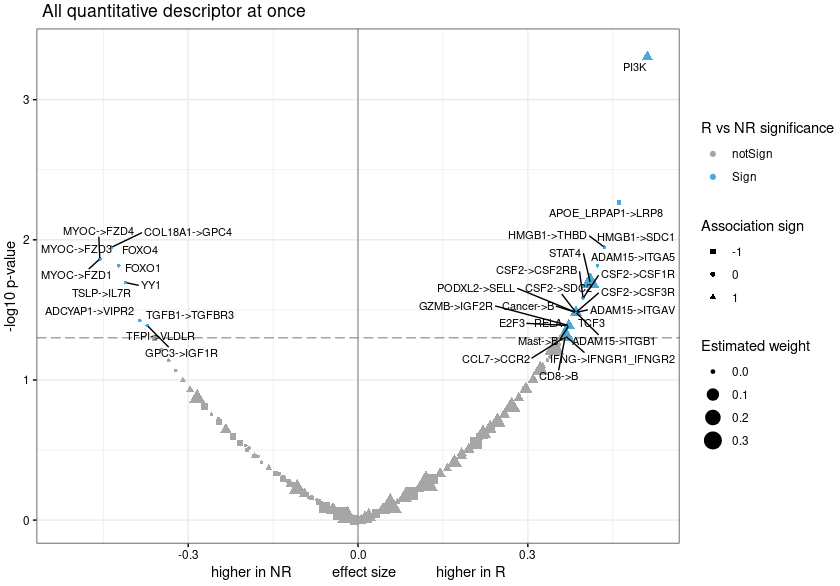
\includegraphics[width=0.95\linewidth,]{easierFinal} \caption{Comparison of genomic features distinguishing patients non-responsive and responsive to immune checkpoint blockade.}\label{fig:easfin}
\end{figure}

This display encapsulates a) the capacity of measurements of
genomic elements to discriminate patients who respond
to ICB for bladder cancer (position of labeled
item on x axis), b) the direction of association of
element activity with immune response (shape of glyph) and c) the
relative magnitudes of weights (size of glyph) estimated for features in
initial model fitting.

The design of this package is noteworthy in its approach
to information hiding. Parameters estimated in machine
learning of tissue-specific relations between quantitative
descriptors of the tumor microenvironment and hallmarks
of immune response are stored in ExperimentHub.

\begin{shaded}
\begin{verbatim}
library(easierData)
list_easierData()
##   eh_id                            title
##  EH6677   Mariathasan2018_PDL1_treatment
##  EH6678                       opt_models
##  EH6679                 opt_xtrain_stats
##  EH6680              TCGA_mean_pancancer
##  EH6681                TCGA_sd_pancancer
##  EH6682                 cor_scores_genes
##  EH6683               intercell networks
##  EH6684                lr_frequency_TCGA
##  EH6685                   group_lr_pairs
##  EH6686                  HGNC_annotation
##  EH6687           scores_signature_genes
\end{verbatim}
\end{shaded}

The structure of the stored model weights resource can be sketched by probing list elements.

\begin{shaded}
\begin{verbatim}
mw = eh[["EH6678"]]
## see ?easierData and browseVignettes('easierData') for documentation
## loading from cache
names(mw)   # TCGA tumor types
##  [1] "LUAD" "LUSC" "BLCA" "BRCA" "CESC" "CRC"  "GBM"  "HNSC" "KIRC"
## [10] "KIRP" "LIHC"   "OV" "PAAD" "PRAD" "SKCM" "STAD" "THCA" "UCEC"
## [19] "NSCLC"
names(mw[["LUAD"]]) # TME descriptors
## [1] "pathways" "immunecells" "tfs" "lrpairs" "ccpairs"
rownames(mw[["LUAD"]]$pathways$CYT) # predict cytolytic activity
##  [1] "(Intercept)" "Androgen" "EGFR" "Estrogen" "Hypoxia"
##  [6]    "JAK-STAT"     "MAPK" "NFkB" "p53"      "PI3K"
## [11]        "TNFa"    "Trail" "VEGF" "WNT"
\end{verbatim}
\end{shaded}


The vignette of the easier package steps through phases,
using these tumor-type-specific weights to compute patient-specific measures
of transcription factor activity or cell-cell interaction on the basis of bulk
RNA-seq (units are transcripts per million), and a patient-specific
measure of pathway activity using raw RNA-seq counts. These metrics
may be of interest in their own right for applications other than
establishing predictions of response to ICB.

Section \ref{app3} provides the names and versions of all packages
used to produce this analysis.



\subsection{Representing and visualizing spatial transcriptomics experiments}\label{representing-and-visualizing-spatial-transcriptomics-experiments}}

Spatial transcriptomics (ST) allows the quantification of RNA expression of large numbers of genes while preserving the spatial context of tissues and cells. This is important as cancer progression depends on a complex tumor microenvironment, and not just cell type composition, but also cell type spatial organization can be used to derive diagnostic or prognostic markers.

The Bioconductor project offers multiple approaches to handle and manipulate\\
spatial transcriptomics (ST) data.
The SpatialExperiment class \cite{rig22} %(Righelli et al. \protect\hyperlink{ref-rig22}{2022}) 
is designed to be a lightweight,
technology-agnostic container. By inheriting from the
SingleCellExperiment class, it unlocks the use in ST data of
analysis packages designed for single-cell data, such as scater for exploration
and QC, and scran for normalization.
SpatialFeatureExperiment \cite{moses23} %(Moses et al. \protect\hyperlink{ref-moses23}{2023}) 
extends SpatialExperiment to easily
reuse polygons and other spatial geometry features from geospatial CRAN
packages, such as sf. See also MoleculeExperiment \cite{Couto2023} %(Couto et al. \protect\hyperlink{ref-Couto2023}{2023}) 
for a different
approach based on the data.table package.

In addition to data containers, Bioconductor provides a rich set of ST data.
The STexampleData and SFEData packages contain a collection of datasets from
different technologies and tissues.
As of December 2023,
the TENxVisiumData package provides a collection of 13 in-house 10X Genomics
Visium datasets from 23 samples across two organisms (human and mouse) and 13
tissues.
The MerfishData package contains two annotated samples assayed with the MERFISH
in-situ imaging protocol.

Finally, Bioconductor offers a growing collection of analysis methods tailored
for spot-based and in-situ ST data, including methods for visualization,
data exploration and quality control, spot deconvolution,
spatially-aware clustering, and identification of spatially-variable genes.

To show a simple example of an analysis workflow on spot-based data,
we explore a fresh frozen
Invasive Ductal Carcinoma breast tissue assayed
with the 10X Genomics Visium platform.
First, we use the ggspavis package for visualization.

%\begin{Shaded}
%\begin{Highlighting}[]
%\KeywordTok{library}\NormalTok{(TENxVisiumData)}
%\CommentTok{\#\# snapshotDate(): 2023{-}10{-}24}
%\KeywordTok{library}\NormalTok{(SpatialExperiment)}
%\CommentTok{\#\# 0/0 packages newly attached/loaded, see sessionInfo() for details.}
%\KeywordTok{library}\NormalTok{(ggspavis)}
%\CommentTok{\#\# 1/1 packages newly attached/loaded, see sessionInfo() for details.}
%\NormalTok{hbc \textless{}{-}}\StringTok{ }\KeywordTok{HumanBreastCancerIDC}\NormalTok{()}
%\CommentTok{\#\# see ?TENxVisiumData and browseVignettes(\textquotesingle{}TENxVisiumData\textquotesingle{}) for documentation}
%\CommentTok{\#\# loading from cache}
%\NormalTok{hbc \textless{}{-}}\StringTok{ }\NormalTok{hbc[,hbc}\OperatorTok{$}\NormalTok{sample\_id}\OperatorTok{==}\StringTok{"HumanBreastCancerIDC1"}\NormalTok{]}
%\NormalTok{hbc}\OperatorTok{$}\NormalTok{in\_tissue \textless{}{-}}\StringTok{ }\OtherTok{TRUE}
%\NormalTok{hbc \textless{}{-}}\StringTok{ }\KeywordTok{rotateImg}\NormalTok{(hbc, }\DataTypeTok{degrees=}\OperatorTok{{-}}\DecValTok{90}\NormalTok{)}
%\KeywordTok{plotVisium}\NormalTok{(hbc, }\DataTypeTok{y\_reverse =} \OtherTok{FALSE}\NormalTok{)}
%\end{Highlighting}
%\end{Shaded}

\begin{shaded}
\begin{verbatim}
library(TENxVisiumData)
## snapshotDate(): 2023-10-24
library(SpatialExperiment)
library(ggspavis)
hbc <- HumanBreastCancerIDC()
## see ?TENxVisiumData and browseVignettes('TENxVisiumData') for documentation
## loading from cache
hbc <- hbc[,hbc$sample_id=="HumanBreastCancerIDC1"]
hbc$in_tissue <- TRUE
hbc <- rotateImg(hbc, degrees=-90)
plotVisium(hbc, y_reverse = FALSE)
\end{verbatim}
\end{shaded}


\begin{figure}
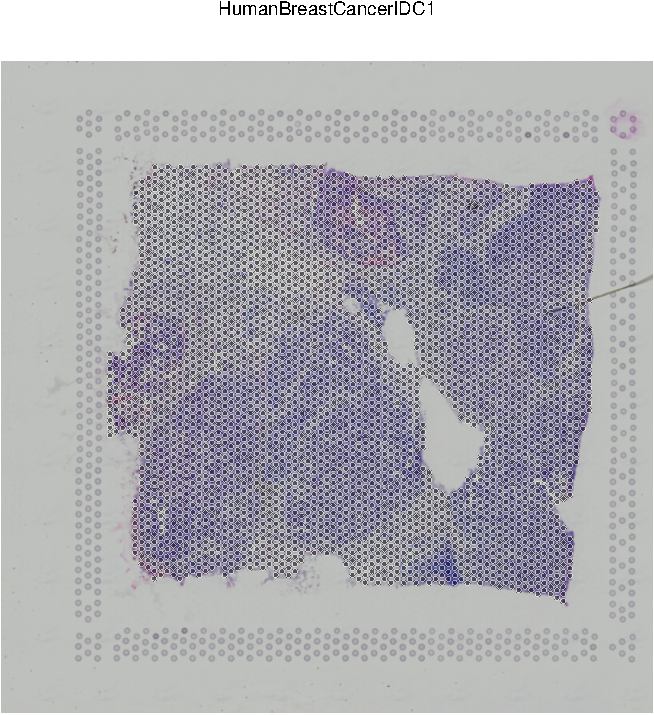
\includegraphics[width=1\linewidth,]{spatpdfs/tenxvisium-1} \caption{Visualization of a Visium breast cancer sample}\label{fig:tenxvisium}
\end{figure}

To investigate the spatially variable genes the nnSVG package
implements a method for the detection of genes whose expression varies in the
tissue spatial domains by fitting nearest-neighbor Gaussian processes 
\cite{webr23}.
%(Weber et al. \protect\hyperlink{ref-webr23}{2023}).

%\begin{Shaded}
%\begin{Highlighting}[]
%\KeywordTok{library}\NormalTok{(scater)}
%\CommentTok{\#\# 2/14 packages newly attached/loaded, see sessionInfo() for details.}
%\KeywordTok{library}\NormalTok{(nnSVG)}
%\CommentTok{\#\# 1/4 packages newly attached/loaded, see sessionInfo() for details.}
%\KeywordTok{library}\NormalTok{(scran)}
%\CommentTok{\#\# 1/9 packages newly attached/loaded, see sessionInfo() for details.}
%
%\CommentTok{\#add quality metrics}
%\NormalTok{is\_mito \textless{}{-}}\StringTok{ }\KeywordTok{grepl}\NormalTok{(}\StringTok{"(\^{}MT{-})|(\^{}mt{-})"}\NormalTok{, }\KeywordTok{rowData}\NormalTok{(hbc)}\OperatorTok{$}\NormalTok{symbol)}
%\NormalTok{hbc \textless{}{-}}\StringTok{ }\KeywordTok{addPerCellQC}\NormalTok{(hbc, }\DataTypeTok{subsets =} \KeywordTok{list}\NormalTok{(}\DataTypeTok{mito =}\NormalTok{ is\_mito))}
%
%\CommentTok{\#\# needed because the column name is hard coded in the nnSVG::filter\_genes}
%\KeywordTok{rowData}\NormalTok{(hbc)}\OperatorTok{$}\NormalTok{gene\_name \textless{}{-}}\StringTok{ }\KeywordTok{rowData}\NormalTok{(hbc)}\OperatorTok{$}\NormalTok{symbol }
%
%\CommentTok{\#\# filter and normalize gene expression}
%\NormalTok{hbc \textless{}{-}}\StringTok{ }\KeywordTok{filter\_genes}\NormalTok{(hbc)}
%\CommentTok{\#\# Gene filtering: removing mitochondrial genes}
%\CommentTok{\#\# removed 13 mitochondrial genes}
%\CommentTok{\#\# Gene filtering: retaining genes with at least 3 counts in at least 0.5\% (n = 19) of spatial locations}
%\CommentTok{\#\# removed 26583 out of 36588 genes due to low expression}
%\NormalTok{hbc \textless{}{-}}\StringTok{ }\KeywordTok{computeLibraryFactors}\NormalTok{(hbc)}
%\NormalTok{hbc \textless{}{-}}\StringTok{ }\KeywordTok{logNormCounts}\NormalTok{(hbc)}
%
%\CommentTok{\#\# select highly variable genes}
%\NormalTok{hvgs \textless{}{-}}\StringTok{ }\KeywordTok{getTopHVGs}\NormalTok{(hbc, }\DataTypeTok{n=}\DecValTok{1000}\NormalTok{)}
%\NormalTok{hbc \textless{}{-}}\StringTok{ }\NormalTok{hbc[hvgs,]}
%
%\CommentTok{\#\# identify spatially variable genes}
%\NormalTok{hbc \textless{}{-}}\StringTok{ }\KeywordTok{nnSVG}\NormalTok{(hbc, }\DataTypeTok{n\_threads=}\DecValTok{4}\NormalTok{)}
%
%\CommentTok{\#\# post{-}processing}
%\NormalTok{hbc \textless{}{-}}\StringTok{ }\NormalTok{hbc[}\KeywordTok{order}\NormalTok{(}\KeywordTok{rowData}\NormalTok{(hbc)}\OperatorTok{$}\NormalTok{rank),]}
%
%\NormalTok{gnr1 \textless{}{-}}\StringTok{ }\KeywordTok{rowData}\NormalTok{(hbc)}\OperatorTok{$}\NormalTok{symbol[}\DecValTok{1}\NormalTok{]}
%\KeywordTok{rownames}\NormalTok{(hbc) \textless{}{-}}\StringTok{ }\KeywordTok{rowData}\NormalTok{(hbc)}\OperatorTok{$}\NormalTok{symbol}
%\end{Highlighting}
%\end{Shaded}

\begin{shaded}
\begin{verbatim}
library(scater)
library(nnSVG)
library(scran)
#add quality metrics
is_mito <- grepl("(ˆMT-)|(ˆmt-)", rowData(hbc)$symbol)
hbc <- addPerCellQC(hbc, subsets = list(mito = is_mito))
## needed because the column name is hard coded in the nnSVG::filter_genes
rowData(hbc)$gene_name <- rowData(hbc)$symbol
## filter and normalize gene expression
hbc <- filter_genes(hbc)
## Gene filtering: removing mitochondrial genes
## removed 13 mitochondrial genes
## Gene filtering: retaining genes with at least 3 counts in at least 0.5% (n = 19) of spatial locations
## removed 26583 out of 36588 genes due to low expression
hbc <- computeLibraryFactors(hbc)
hbc <- logNormCounts(hbc)
## select highly variable genes
hvgs <- getTopHVGs(hbc, n=1000)
hbc <- hbc[hvgs,]
## identify spatially variable genes
hbc <- nnSVG(hbc, n_threads=4)
## post-processing
hbc <- hbc[order(rowData(hbc)$rank),]
gnr1 <- rowData(hbc)$symbol[1]
rownames(hbc) <- rowData(hbc)$symbol
\end{verbatim}
\end{shaded}

By ranking the results of nnSVG, we are able to detect the most spatially
variable genes. As an example, we show how the most spatially variable gene varies
across the tissue.

%\begin{Shaded}
%\begin{Highlighting}[]
%\KeywordTok{plotVisium}\NormalTok{(hbc, }\DataTypeTok{y\_reverse =} \OtherTok{FALSE}\NormalTok{, }\DataTypeTok{fill =}\NormalTok{ gnr1, }\DataTypeTok{palette=}\StringTok{"red"}\NormalTok{)}
%\end{Highlighting}
%\end{Shaded}

\begin{shaded}
\begin{verbatim}
plotVisium(hbc, y_reverse = FALSE, fill = gnr1, palette="red")
\end{verbatim}
\end{shaded}

\begin{figure}
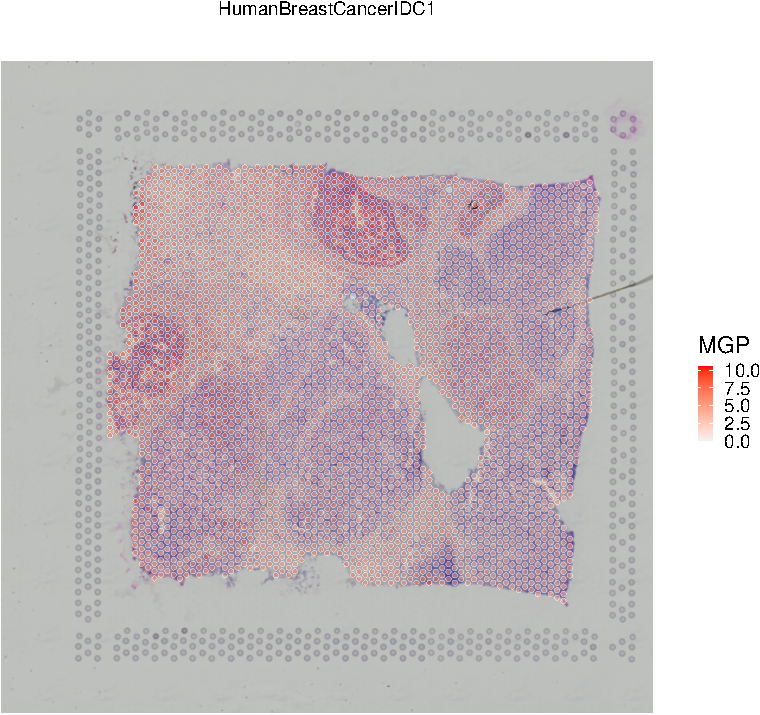
\includegraphics[width=1\linewidth,]{spatpdfs/plotvisium-1} \caption{Spatial expression of a highly variable gene}\label{fig:plotvisium}
\end{figure}

Finally, we show an example of an in-situ ST technology, by visualizing a breast
cancer sample assayed with the 10X Genomics Xenium platform.

\begin{shaded}
\begin{verbatim}
library(SpatialFeatureExperiment)
library(SFEData)
jbr = JanesickBreastData("rep1")
jbr
## class: SpatialFeatureExperiment
## dim: 541 167782
## metadata(1): Samples
## assays(1): counts
## rownames(541): ABCC11 ACTA2 ... BLANK_0497 BLANK_0499
## rowData names(6): ID Symbol ... vars cv2
## colnames: NULL
## colData names(10): Sample Barcode ... nCounts nGenes
## reducedDimNames(0):
## mainExpName: NULL
## altExpNames(0):
## spatialCoords names(2) : x_centroid y_centroid
## imgData names(1): sample_id
##
## unit:
## Geometries:
## colGeometries: centroids (POINT), cellSeg (POLYGON), nucSeg (GEOMETRY)
##
## Graphs:
## sample01:
\end{verbatim}
\end{shaded}

%\begin{Shaded}
%\begin{Highlighting}[]
%\KeywordTok{library}\NormalTok{(SpatialFeatureExperiment)}
%\KeywordTok{library}\NormalTok{(SFEData)}
%\NormalTok{jbr =}\StringTok{ }\KeywordTok{JanesickBreastData}\NormalTok{(}\StringTok{"rep1"}\NormalTok{)}
%\NormalTok{jbr}
%\CommentTok{\#\# class: SpatialFeatureExperiment }
%\CommentTok{\#\# dim: 541 167782 }
%\CommentTok{\#\# metadata(1): Samples}
%\CommentTok{\#\# assays(1): counts}
%\CommentTok{\#\# rownames(541): ABCC11 ACTA2 ... BLANK\_0497 BLANK\_0499}
%\CommentTok{\#\# rowData names(6): ID Symbol ... vars cv2}
%\CommentTok{\#\# colnames: NULL}
%\CommentTok{\#\# colData names(10): Sample Barcode ... nCounts nGenes}
%\CommentTok{\#\# reducedDimNames(0):}
%\CommentTok{\#\# mainExpName: NULL}
%\CommentTok{\#\# altExpNames(0):}
%\CommentTok{\#\# spatialCoords names(2) : x\_centroid y\_centroid}
%\CommentTok{\#\# imgData names(1): sample\_id}
%\CommentTok{\#\# }
%\CommentTok{\#\# unit:}
%\CommentTok{\#\# Geometries:}
%\CommentTok{\#\# colGeometries: centroids (POINT), cellSeg (POLYGON), nucSeg (GEOMETRY) }
%\CommentTok{\#\# }
%\CommentTok{\#\# Graphs:}
%\CommentTok{\#\# sample01:}
%\end{Highlighting}
%\end{Shaded}

We can leverage the nature of in-situ data to explore the cell density across the
tissue, identifying the tissue's macrostructure, and the cell segmentation,
zooming in on a small portion of the tissue.

\begin{shaded}
\begin{verbatim}
library(Voyager)
cellbins <- plotCellBin2D(jbr, hex = TRUE)
cellgeo <- plotGeometry(jbr, "cellSeg", bbox=c("xmin"=0, "ymin"=4000, "xmax"=1000, "ymax"=5000))
library(gridExtra)
grid.arrange(cellbins, cellgeo, ncol=2)
\end{verbatim}
\end{shaded}

\begin{figure}
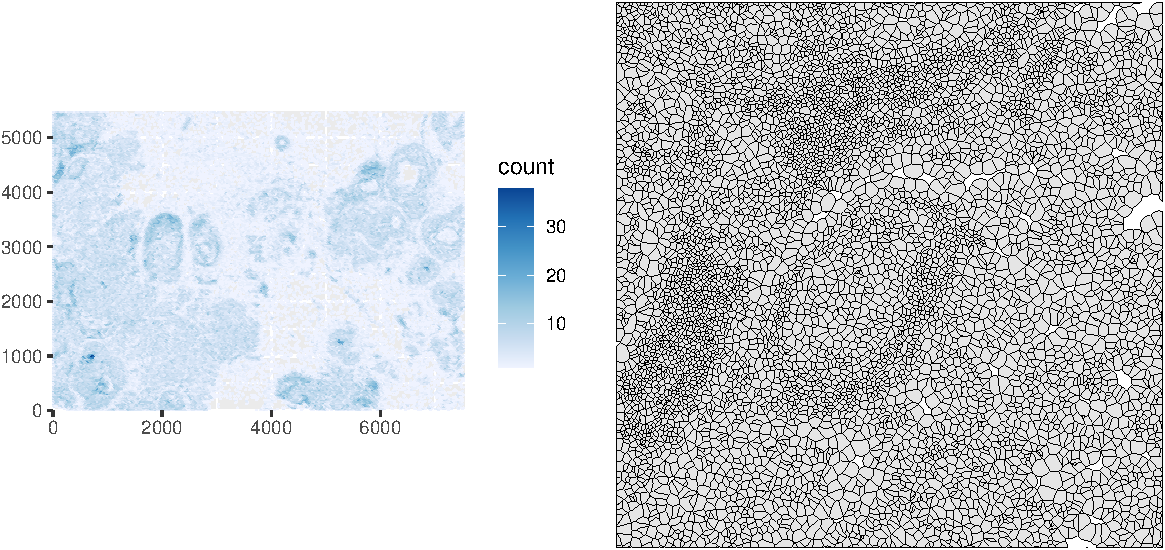
\includegraphics[width=1\linewidth,]{spatpdfs/plotvoyager-1} \caption{Cell density and cell boundaries of a Xenium breast cancer sample}\label{fig:plotvoyager}
\end{figure}

Finally, we can visualize the expression of marker genes after log-normalizing
the data.

\begin{shaded}
\begin{verbatim}
jbr <- jbr[, jbr$nCounts >= 20]
jbr <- logNormCounts(jbr)
library(scattermore)
## 1/0 packages newly attached/loaded, see sessionInfo() for details.
strom <- plotSpatialFeature(jbr, "POSTN", colGeometryName = "centroids",
scattermore = TRUE, ncol = 2, pointsize = 0.5) + ggtitle("POSTN, stromal")
fasn <- plotSpatialFeature(jbr, "FASN", colGeometryName = "centroids",
scattermore = TRUE, ncol = 2, pointsize = 0.5) +
ggtitle("FASN, invasive")
grid.arrange(strom, fasn, ncol=2)
\end{verbatim}
\end{shaded}

%\begin{Shaded}
%\begin{Highlighting}[]
%\NormalTok{jbr \textless{}{-}}\StringTok{ }\NormalTok{jbr[, jbr}\OperatorTok{$}\NormalTok{nCounts }\OperatorTok{\textgreater{}=}\StringTok{ }\DecValTok{20}\NormalTok{]}
%\NormalTok{jbr \textless{}{-}}\StringTok{ }\KeywordTok{logNormCounts}\NormalTok{(jbr)}
%\KeywordTok{library}\NormalTok{(scattermore)}
%\CommentTok{\#\# 1/0 packages newly attached/loaded, see sessionInfo() for details.}
%\NormalTok{strom \textless{}{-}}\StringTok{ }\KeywordTok{plotSpatialFeature}\NormalTok{(jbr, }\StringTok{"POSTN"}\NormalTok{, }\DataTypeTok{colGeometryName =} \StringTok{"centroids"}\NormalTok{,}
%                   \DataTypeTok{scattermore =} \OtherTok{TRUE}\NormalTok{, }\DataTypeTok{ncol =} \DecValTok{2}\NormalTok{, }\DataTypeTok{pointsize =} \FloatTok{0.5}\NormalTok{) }\OperatorTok{+}
%\StringTok{  }\KeywordTok{ggtitle}\NormalTok{(}\StringTok{"POSTN, stromal"}\NormalTok{)}
%
%\NormalTok{fasn \textless{}{-}}\StringTok{ }\KeywordTok{plotSpatialFeature}\NormalTok{(jbr, }\StringTok{"FASN"}\NormalTok{, }\DataTypeTok{colGeometryName =} \StringTok{"centroids"}\NormalTok{,}
%                   \DataTypeTok{scattermore =} \OtherTok{TRUE}\NormalTok{, }\DataTypeTok{ncol =} \DecValTok{2}\NormalTok{, }\DataTypeTok{pointsize =} \FloatTok{0.5}\NormalTok{) }\OperatorTok{+}
%\StringTok{  }\KeywordTok{ggtitle}\NormalTok{(}\StringTok{"FASN, invasive"}\NormalTok{)}
%
%\KeywordTok{grid.arrange}\NormalTok{(strom, fasn, }\DataTypeTok{ncol=}\DecValTok{2}\NormalTok{)}
%\end{Highlighting}
%\end{Shaded}

\begin{figure}
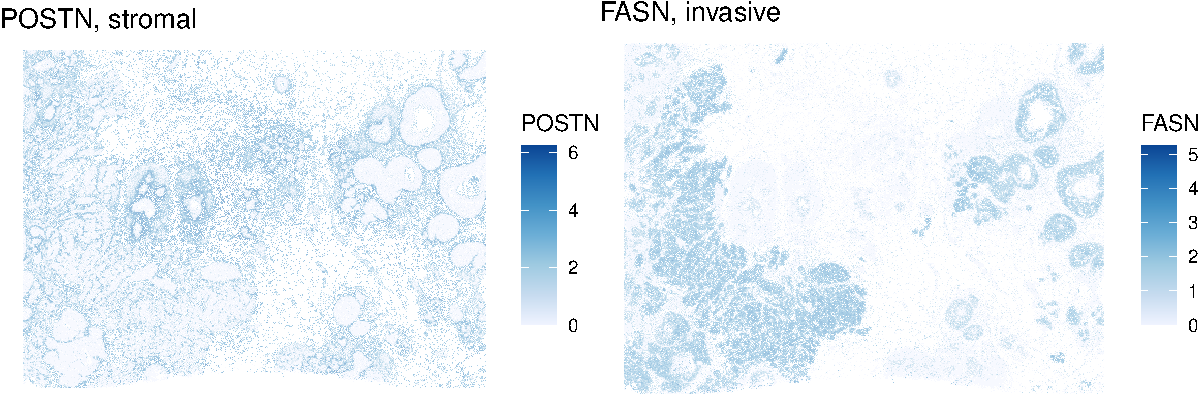
\includegraphics[width=1\linewidth,]{spatpdfs/sfemark-1} \caption{Spatial expression of marker genes}\label{fig:sfemark}
\end{figure}



\section{Components and processes for introducing new data, analytic tools, documents}\label{class}

\subsection{Contributions and review}\label{contributions-and-review}

Proposed contributions to Bioconductor's ecosystem of software packages,
data resources, and documentation are registered at
\begin{verbatim}
https://github.com/bioconductor/contributions/issues 
\end{verbatim}
Contributors
identify a public github.com repository that houses
their software, or some durable open data repository
for a data contribution. The contributor
provides schematized information on format, licensing, and commitment
to maintenance of the contributed resource. After a series of
automated and manual verification steps, the contributed
resource enters the review process.

An example under review in December 2023 is the ``methodical''
package, submitted 27 September 2023. The issue number
at the contributions site is 3169. This contribution is of
particular interest as it addresses new data resources from
whole genome and reduced representation bisulfite sequencing
experiments. Specifics on these high-resolution studies
of DNA methylation
in a variety of clinical situtions are given below.

\subsection{Data structures}\label{data-structures}

Inheritance is a key feature of object-oriented programming (OOP) that allows us to define a new class out of existing classes and add new features, which provides reusability of code. Inheritance carries over attributes and methods defined for base classes; `Attributes' are variables that are bound in a class. They are used to define behavior and methods for objects of that class. `Methods' are functions defined within a class that receive an instance of the class, conventionally called self, as the first argument. The attributes defined for a base class will automatically be present in the derived class, and the methods for the base class will work for the derived class. The R programming language has three different class systems: S3, S4, and Reference. Inheritance in S3 classes does not have any fixed definition, and hence attributes of S3 objects can be arbitrary. Derived classes, however, inherit the methods defined for the base class. Inheritance in S4 classes is more structured, and derived classes inherit both attributes and methods of the parent class. Reference classes are similar to S4 classes, but they are mutable and have reference semantics.

S4 classes are used extensively in Bioconductor to create data structures that store complex information, such as biological assay data and metadata, in one or more slots. The entire structure can then be assigned to an R object, and the types of information in each slot of the object are tightly controlled. S4 generics and methods define functions that can be applied to these objects, providing a rich software development infrastructure while ensuring interoperability, reusability, and efficiency.

Bioconductor have established Bioconductor classes to represent different types of biological data. Data and tools distributed through Bioconductor adopt Bioconductor classes, providing convenient methods and improving usability and interoperability within the Bioconductor ecosystem.

\begin{table}
\caption{Overview of key datatypes and associated classes in Bioconductor.}
\begin{tabular}[t]{ll}
\toprule
Data Types & Bioconductor Classes\\
\midrule
Genomic coordinates (1-based, closed interval) & GRanges\\
Groups of genomic coordinates & GRangesList\\
Ragged genomic coordinates & RaggedExperiment\\
Gene sets & GeneSet\\
Rectangular Features x samples & SummarizedExperiment\\
\addlinespace
Multi-omics data & MultiAssayExperiment\\
Single-cell data & SingleCellExperiment\\
Spatial Transcriptomics & SpatialExperiment\\
Mass spectrometry data & Spectra\\
\bottomrule
\end{tabular}
\end{table}

The GRanges class represents a collection of genomic ranges and associated annotations. Each element in the vector represents a set genomic ranges in terms of the sequence name (seqnames, typically the chromosome), start and end coordinates (ranges, as an IRanges object), strand (strand, either positive, negative, or unstranded), and optional metadata columns (e.g., exon\_id and exon\_name in the below).

\begin{verbatim}
GRanges object with 4 ranges and 2 metadata columns:
      seqnames            ranges strand |   exon_id       exon_name
         <Rle>         <IRanges>  <Rle> | <integer>     <character>
  [1]        X 99883667-99884983      - |    667145 ENSE00001459322
  [2]        X 99885756-99885863      - |    667146 ENSE00000868868
  [3]        X 99887482-99887565      - |    667147 ENSE00000401072
  [4]        X 99887538-99887565      - |    667148 ENSE00001849132
  -------
  seqinfo: 722 sequences (1 circular) from an unspecified genome
\end{verbatim}

The GRangesList object serves as a container for genomic features consisting of multiple
ranges that are grouped by a parent features, such as spliced transcripts that are
comprised of exons. A GRangesList object behaves like a list and many of the same
methods for GRanges objects are available for GRangesList object as well.

The SummarizedExperiment class (see Figure \ref{fig:sesc} is a matrix-like container, where rows represent features of interest (e.g., genes, transcripts, exons, etc.) and columns represent samples. The attributes of this object include experimental results (in assays), information on observations (in rowData) and samples (in colData), and additional metadata (in metadata). SummarizedExperiment objects can simultaneouly manage several experimental results as long as they are of the same dimensions. The best benefit of using SummarizedExperiment class is the coordination of the metadata and assays when subsetting. SummarizedExperiment is similar to the historical ExpressionSet class, but more flexible in its row information, allowing both GRanges and DataFrames. ExpressionSet object can be easily converted to SummarizedExperiment.

RangedSummarizedExperiment inherits the SummarizedExperiment class, with the extended capability of storing genomic ranges (as a GRanges or GRangesList object) of interest instead of a DataFrame (S4-class objectcs similar to data.frame) of features in rows.

The MultiAssayExperiment class (presented above in
Figure \ref{fig:masc}) is modeled after the SummarizedExperiment class.
A MultiAssayExperiment instance \texttt{M} can be
filtered as a three-dimensional array.
When \texttt{G} is a vector of feature identifiers,
\texttt{C} a vector of sample identifiers, and \texttt{E} a
vector of experiment names, then \texttt{M{[}G, C, E{]}} is
a MultiAssayExperiment with content restricted to the
requested features, samples, and experiments. The MultiAssayExperiment
package includes tooling to convert data content to ``long'' or
``wide'' formats. In long format, each element of the assay array occupies
a row, accompanied by metadata associated with the element.
In wide format, each sample occupies a row, accompanied by all
assocated assay and metadata elements.

\subsection{Out-of-memory data representation strategies}\label{out-of-memory-data-representation-strategies}

We return to the ``methodical'' package
submission mentioned above.
A number of whole-genome bisulfite sequencing experiments on
tumors from various anatomic sites are available
in ExperimentHub.
Metadata in that package shows that the datasets
are large, ranging from 2-40 gigabytes. One smaller
dataset is provided for illustration.

%\begin{Shaded}
%\begin{Highlighting}[]
%\KeywordTok{library}\NormalTok{(TumourMethData)}
%\NormalTok{demm =}\StringTok{ }\KeywordTok{download\_meth\_dataset}\NormalTok{(}\StringTok{"mcrpc\_wgbs\_hg38\_chr11"}\NormalTok{)}
%\CommentTok{\#\# [1] "A HDF5 SummarizedExperiment is already present in /home/vincent/TEMP/RtmpIQh7nv/mcrpc\_wgbs\_hg38\_chr11 and is being returned"}
%\NormalTok{demm}
%\CommentTok{\#\# class: RangedSummarizedExperiment }
%\CommentTok{\#\# dim: 1333114 100 }
%\CommentTok{\#\# metadata(5): genome is\_h5 ref\_CpG chrom\_sizes descriptive\_stats}
%\CommentTok{\#\# assays(2): beta cov}
%\CommentTok{\#\# rownames: NULL}
%\CommentTok{\#\# rowData names(0):}
%\CommentTok{\#\# colnames(100): DTB\_003 DTB\_005 ... DTB\_265 DTB\_266}
%\CommentTok{\#\# colData names(4): metastatis\_site subtype age sex}
%\KeywordTok{rowRanges}\NormalTok{(demm)}
%\CommentTok{\#\# GRanges object with 1333114 ranges and 0 metadata columns:}
%\CommentTok{\#\#             seqnames    ranges strand}
%\CommentTok{\#\#                \textless{}Rle\textgreater{} \textless{}IRanges\textgreater{}  \textless{}Rle\textgreater{}}
%\CommentTok{\#\#         [1]    chr11     60077      *}
%\CommentTok{\#\#         [2]    chr11     60088      *}
%\CommentTok{\#\#         [3]    chr11     60365      *}
%\CommentTok{\#\#         [4]    chr11     60941      *}
%\CommentTok{\#\#         [5]    chr11     60979      *}
%\CommentTok{\#\#         ...      ...       ...    ...}
%\CommentTok{\#\#   [1333110]    chr11 135076482      *}
%\CommentTok{\#\#   [1333111]    chr11 135076496      *}
%\CommentTok{\#\#   [1333112]    chr11 135076502      *}
%\CommentTok{\#\#   [1333113]    chr11 135076507      *}
%\CommentTok{\#\#   [1333114]    chr11 135076510      *}
%\CommentTok{\#\#   {-}{-}{-}{-}{-}{-}{-}}
%\CommentTok{\#\#   seqinfo: 25 sequences from an unspecified genome; no seqlengths}
%\KeywordTok{names}\NormalTok{(}\KeywordTok{colData}\NormalTok{(demm))}
%\CommentTok{\#\# [1] "metastatis\_site" "subtype"         "age"             "sex"}
%\KeywordTok{table}\NormalTok{(demm}\OperatorTok{$}\NormalTok{metastatis\_site)}
%\CommentTok{\#\# }
%\CommentTok{\#\#       Bone      Liver Lymph\_node      Other }
%\CommentTok{\#\#         43         11         38          8}
%\end{Highlighting}
%\end{Shaded}

\begin{shaded}
\begin{verbatim}
library(TumourMethData)
demm = download_meth_dataset("mcrpc_wg ..." ... [TRUNCATED] 
demm
## class: RangedSummarizedExperiment 
## dim: 1333114 100 
## metadata(5): genome is_h5 ref_CpG chrom_sizes descriptive_stats
## assays(2): beta cov
## rownames: NULL
## rowData names(0):
## colnames(100): DTB_003 DTB_005 ... DTB_265 DTB_266
## colData names(4): metastatis_site subtype age sex
rowRanges(demm)
## GRanges object with 1333114 ranges and 0 metadata columns:
##             seqnames    ranges strand
##                <Rle> <IRanges>  <Rle>
##         [1]    chr11     60077      *
##         [2]    chr11     60088      *
##         [3]    chr11     60365      *
##         [4]    chr11     60941      *
##         [5]    chr11     60979      *
##         ...      ...       ...    ...
##   [1333110]    chr11 135076482      *
##   [1333111]    chr11 135076496      *
##   [1333112]    chr11 135076502      *
##   [1333113]    chr11 135076507      *
##   [1333114]    chr11 135076510      *
##   -------
##   seqinfo: 25 sequences from an unspecified genome; no seqlengths
names(colData(demm))
## [1] "metastatis_site" "subtype"         "age"             "sex"            
table(demm$metastatis_site)
##      Bone      Liver Lymph_node      Other 
##        43         11         38          8 
\end{verbatim}
\end{shaded}


References to \texttt{demm} involve an 800MB excerpt of a
prostate cancer atlas with a
storage footprint of 40GB.
Ideally,
queries about particular genomic
regions on particular samples, whole-sample statistical summaries,
and searches for patterns can be carried out without
specific accommodation of the data size or representation.
The DelayedArray package helps pursue this aim. We'll illustrate
by interrogating the prostate cancer WGBS data for ``beta''
(fraction of locus that is methylated) values in the vicinity of
gene ATM.

\begin{shaded}
\begin{verbatim}
library(EnsDb.Hsapiens.v86)
gg = genes(EnsDb.Hsapiens.v86)
# get gene addresses
atmpos = gg[gg$gene_name == "ATM" &
gg$gene_biotype == "protein_coding"] # filter to ATM
seqlevelsStyle(atmpos) = "UCSC"
assay(subsetByOverlaps(demm, atmpos+1e6))
## <18110 x 100> DelayedMatrix object of type "double":
##          DTB_003 DTB_005 DTB_008 ... DTB_265 DTB_266
##     [1,]  0.1053  0.7660  0.9206   .  0.6944  0.9412
##     [2,]  0.4062  0.9091  0.9318   .  0.5676  1.0000
##     [3,]  0.1379  0.0000  0.7400   .  0.4643  0.9231
##     [4,]  0.2308  0.9231  0.9149   .  0.8929  0.9286
##     [5,]  0.1481  0.8500  0.8864   .  0.8710  0.9762
##      ...       .       .       .   .       .       .
## [18106,]  0.4138  0.3143  0.3208   . 0.17647 0.10000
## [18107,]  0.2727  0.2745  0.4143   . 0.22500 0.32500
## [18108,]  0.2258  0.4800  0.5775   . 0.08889 0.25000
## [18109,]  0.5278  0.7059  0.8088   . 0.55263 0.97561
## [18110,]  0.2778  0.3137  0.6957   . 0.52632 0.35714
\end{verbatim}
\end{shaded}


The numeric values presented above are just the
``corners'' of the associated array, presented as a ``check''
on the content requested. Transfer of array content to
the CPU for numerical analysis only occurs on demand,
which can be tailored to the quantity of RAM available
at analysis time.

\subsection{Quality assessment of Bioconductor resources}\label{quality-assessment-of-bioconductor-resources}

Figure \ref{fig:qapic} is an overview of the periodic ecosystem
testing process for Bioconductor software packages in the
release branch. All Bioconductor
and CRAN packages on which they depend are present and are updated
on change to sources.

\begin{figure}
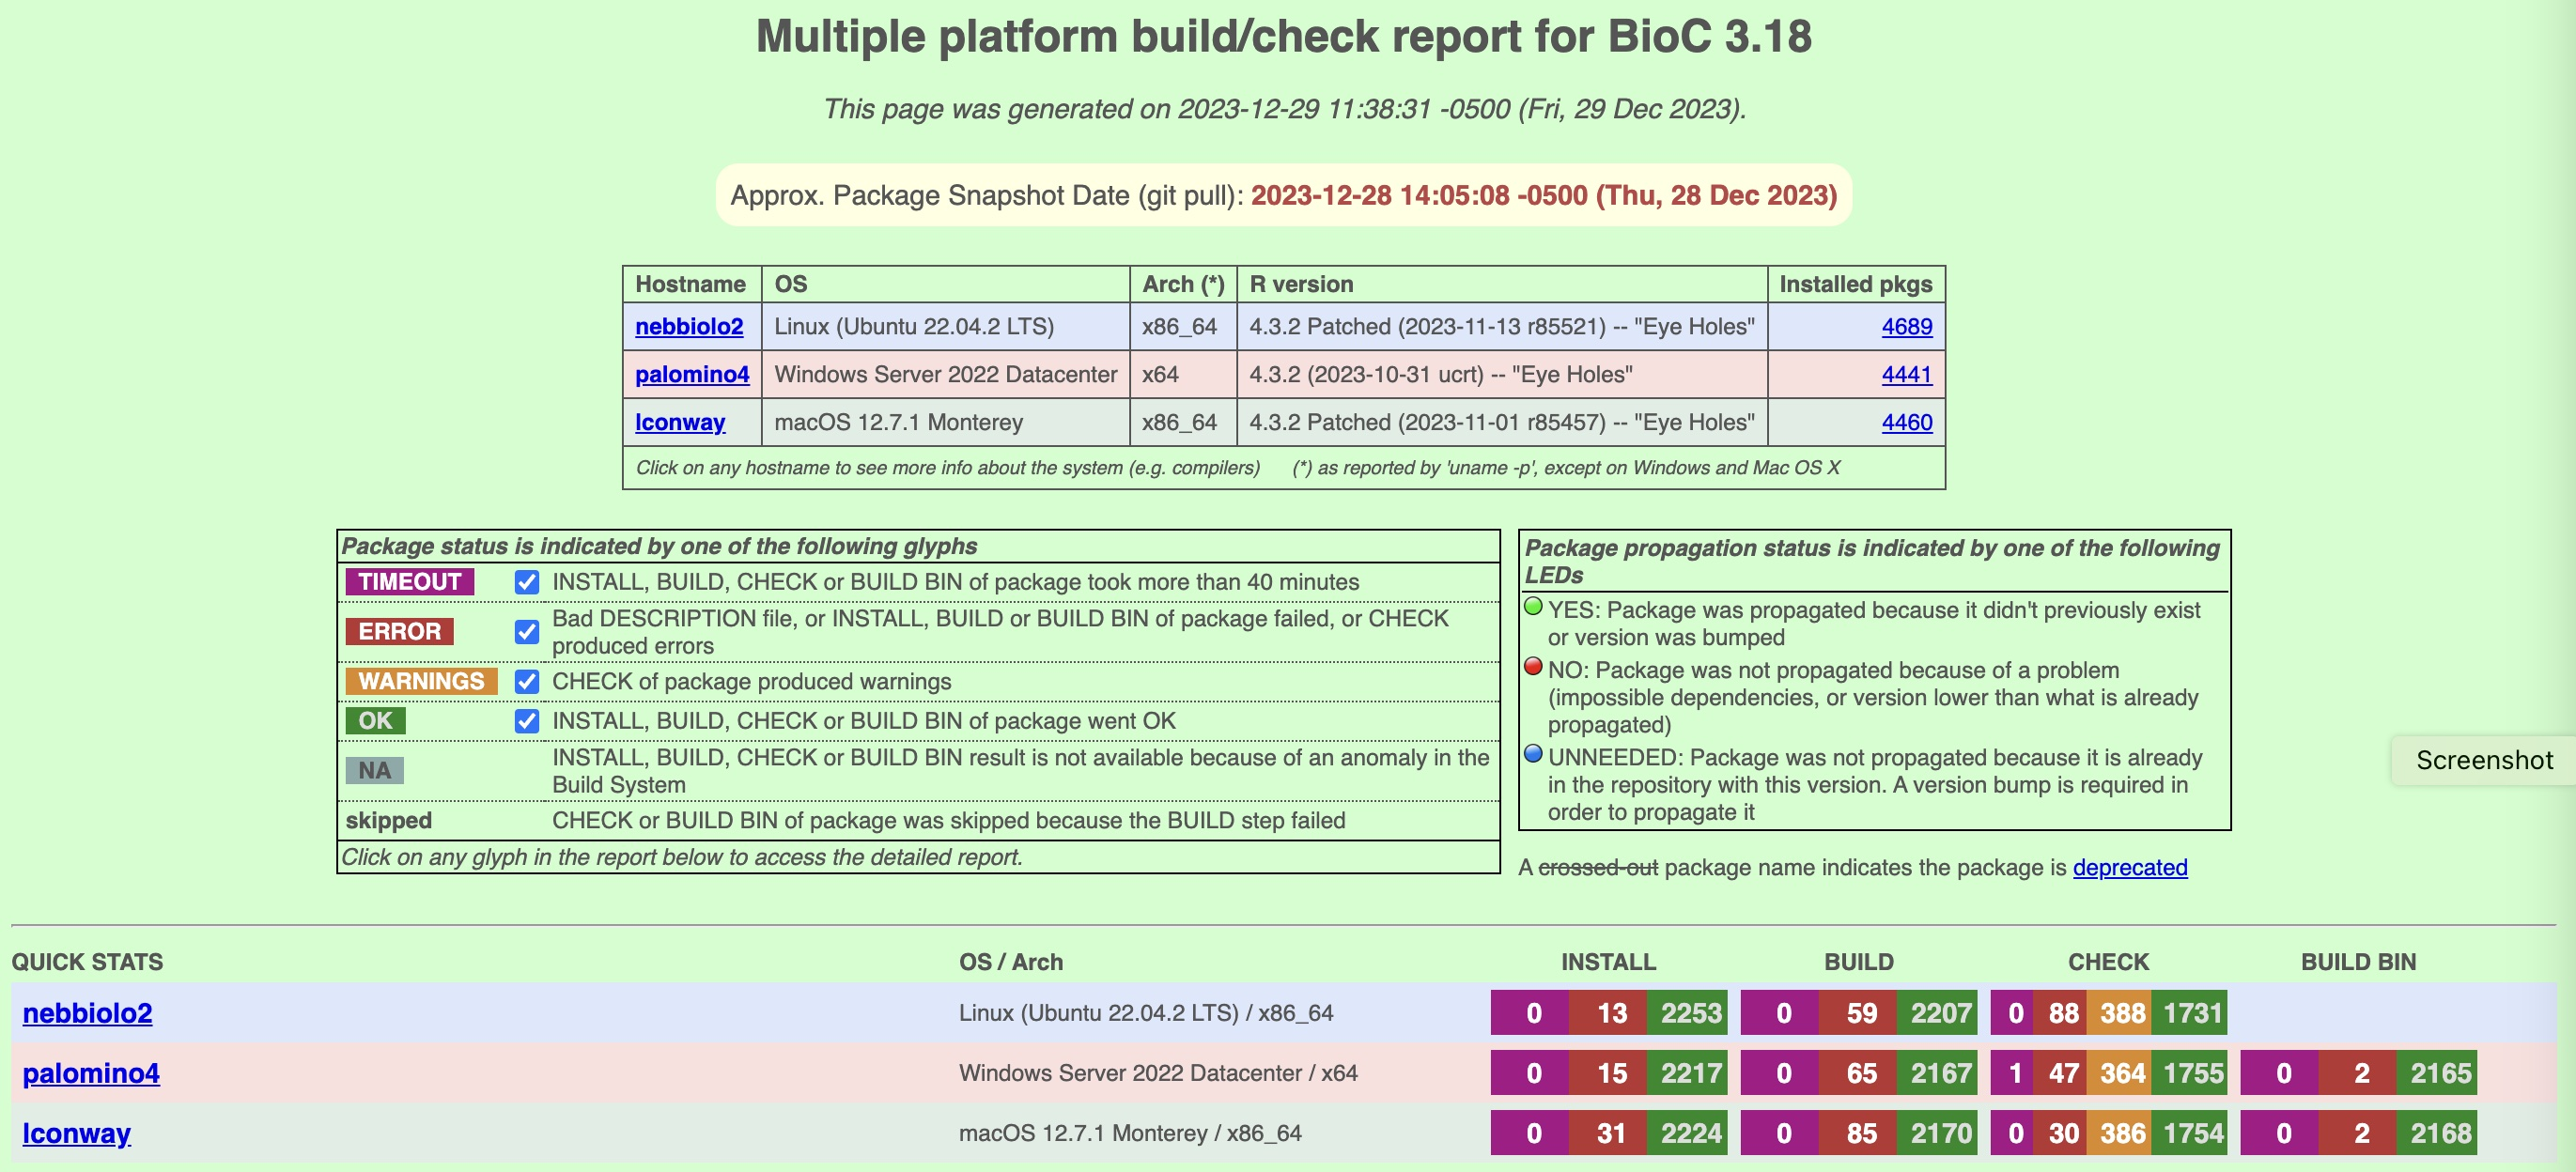
\includegraphics[width=1.21\linewidth,]{QApage} \caption{Build report for Bioc 3.18, 12-29-2023.}\label{fig:qapic}
\end{figure}

The project distributes source tarballs for Linux-like systems, and
compiled binaries for MacOS and Windows. Numbers in red boxes indicate
failures to install, build, or check. Failure events are
frequently platform-specific; full logs are provided
on the build report pages to help developers isolate and fix
build and check errors. When failures are persistent, developers
are contacted by core. If contact cannot be made and failures
continue, packages are deprecated for at least one release, and
then removed.

\section{Pedagogics and workforce development}\label{pedagogics-and-workforce-development}

The Bioconductor project has undertaken a number
of initiatives to support growth of the
scientific workforce's capacity to efficiently
integrate and interpret
genome-scale experiments.

\begin{itemize}
\item
  \textbf{Partnering with The Carpentries.} The Carpentries \url{https://carpentries.org} is a non-profit organization focused on teaching programming
  and data science to researchers. The organization defines ``good
  practices in lesson design and development, and open source
  collaboration skills''. Bioconductor community members have
  created bioc-intro, bioc-project, and bioc-rnaseq repositories
  using The Carpentries Incubator template. This arrangement helps
  Bioconductor create and manage a ``train the trainer'' process
  according to tested pedagogical principles.
\item
  \textbf{Curating monographs for topics in genomic data science.} The
  breadth of Bioconductor resources for genomics, combined with the
  energetic approach to software and annotation upkeep in the project,
  empowers Bioconductor developers to produce unified, wide-ranging,
  computable documents on topics of interest to the broader
  cancer genomics community. Books currently available
  at bioconductor.org include OSCA (Orchestrating Single Cell Analysis
  with Bioconductor), SingleRBook (Assigning cell types with SingleR),
  csawBook (Analysis of ChIP-seq data), OHCA (Orchestrating Hi-C
  Analysis with Bioconductor) and R for Mass Spectrometry. Very
  recently, Jacques Serizay of Institut Pasteur has contributed
  a book authoring framework called BiocBook. This transforms documents
  marked up in Posit's quarto format into web-based books backed up by Docker
  containers and maintained with templated GitHub actions. The
  OHCA book is produced and managed with BiocBook.
\item
  \textbf{A system for authoring and deploying interactive workshops.}
\end{itemize}

Figure \ref{fig:wssc} gives an overview of the resources and
objectives of the system underlying \url{workshop.bioconductor.org}.
Given a kubernetes-enabled cluster
the workshop system assembles

\begin{itemize}
\tightlist
\item
  compute and storage elements,
\item
  static components (training texts and shareable data),
\item
  development environments (containers with all runtime elements
  required to compiled code, conduct analyses, communicate with GPUs).
\end{itemize}

\begin{figure}
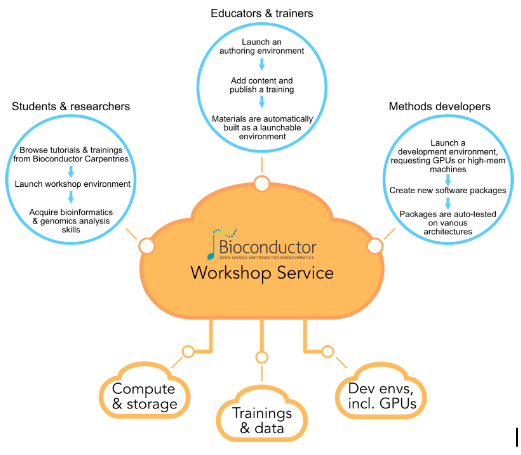
\includegraphics[width=0.8\linewidth,]{WorkshopSCHEMA} \caption{Workshop.bioconductor.org schematic.}\label{fig:wssc}
\end{figure}

A lightly customized deployment of the Galaxy system (usegalaxy.org)
is used to deal with authentication
and process initiation and termination.

This system has been used to serve interactive workshops in a number
of international conferences. Content in R markdown or quarto
can be produced by anyone interested in offering a workshop, and
the ``BiocWorkshopSubmit'' app at workshop.bioconductor.org
can be used to identify new content to the system. Markdown
documents will be analyzed to determine what resources are needed
for the containerization of workshop software and data components,
and the container will be created and registered at the GitHub
Container Registry. Arrangements to deploy the workshop over
a given calendar period can be made with Bioconductor core. The
workshop container can be used to conduct the workshop on any
system with a Docker client.

\section{Conclusions and paths forward}\label{conclusions-and-paths-forward}

We have described several aspects of
Bioconductor's approach to ecosystem management for cancer
genomics data science resources. In light of
the dynamism
of biotechnological innovation, it is clear that the project
must anticipate change. But it is challenging to introduce
changes to processes on which a very large community depends
for their daily research work. Commitments to supporting reproducible
research entail that Bioconductor preserves decades worth of images
of software and data for immediate retrieval via
web request by parties unknown
to the project.

We'll conclude this report with a few observations on
general paths that the project is likely to take that
should have favorable consequences to researchers in
cancer genomics.

\begin{itemize}
\item
  \textbf{Language-agnostic data and annotation} The \texttt{alabaster.*} packages
  introduced in Bioconductor 3.17 are designed to convert existing
  Bioconductor data structures to formats that are more readily ingested
  by software in other languages. Thus the \texttt{alabaster.mae}
  package will convert a MultiAssayExperiment into a collection
  of files of metadata (serialized in JSON), sample-level data
  (serialized as CSV), and assay data (serialized to HDF5).
\item
  \textbf{Zero-configuration genomic analysis environments} Users
  of Docker containers have long been able to take advantage of
  Bioconductor containers pre-populated with Rstudio and runtime
  resources to support installation of any desired software packages.
  The bioc2u system (\url{https://github.com/bioconductor/bioc2u}) in conjunction
  with r2u (\url{github.com/eddelbuettel/r2u}) introduces the
  availability of Debian packages for all Bioconductor packages,
  made available in a CRAN-like repository. Given a system running
  Ubuntu 22 or 20, the apt package manager will resolve any package
  requests with tested, fully linked binary packages. Users do not
  have to perform any configuration or compilation of system
  utilities or package code. This practice can greatly reduce
  resource consumption that occurs when individuals or
  workflow systems need to compile
  every package and its dependencies to perform analyses.
\item
  \textbf{Computation at the data} Several members of Bioconductor's
  development core are on the technical development team of
  NHGRI's Analysis and Visualization Laboratory (AnVIL). The aim
  of this project is to overthrow the prevalent model of downloading data for
  local analysis. AnVIL mobilizes commercial cloud computing and
  storage to support truly elastic genomic analysis -- create and
  pay for only the computation you need. The basic
  strategy is described in Schatz et al. (\protect\hyperlink{ref-Schatz2022}{2022}). This system was
  used in the production of the Telomere-to-Telomere
  genome build, see Aganezov et al. (\protect\hyperlink{ref-Aganezov2022}{2022}).
\end{itemize}

We hope that the project can continue to support researchers in cancer
genomics for another 20 years!

%\section{Acknowledgments}\label{acknowledgments}
%
%%This work was supported in part by NIH NCI 3U24CA180996-10S1, NHGRI 5U24HG004059-18, and NSF ACCESS allocation BIR190004.


%\pagebreak

%\section{Bioconductor software packages with `cancer' in package description}\label{app1}

Quoted text is the content of the Description element of the package DESCRIPTION. Names following the
text are as reported in the Authors field.

\begin{longtable}[t]{l>{\raggedright\arraybackslash}p{25em}}
\toprule
package & desc\\
\midrule
AMARETTO & "Integrating an increasing number of available multi-omics
cancer data remains one of the main challenges to improve our
understanding of cancer. One of the main challenges is using
multi-omics data for identifying novel cancer driver genes. We
have developed an algorithm, called AMARETTO, that integrates
copy number, DNA methylation and gene expression data to
identify a set of driver genes by analyzing cancer samples and
connects them to clusters of co-expressed genes, which we
define as modules. We applied AMARETTO in a pancancer setting
to identify cancer driver genes and their modules on multiple
cancer sites. AMARETTO captures modules enriched in
angiogenesis, cell cycle and EMT, and modules that accurately
predict survival and molecular subtypes. This allows AMARETTO
to identify novel cancer driver genes directing canonical
cancer pathways." --Jayendra Shinde, Celine Everaert, Shaimaa Bakr, Mohsen Nabian, Jishu Xu, Vincent Carey, Nathalie Pochet, Olivier Gevaert\\
BaalChIP & "The package offers functions to process multiple ChIP-seq
BAM files and detect allele-specific events. Computes allele
counts at individual variants (SNPs/SNVs), implements extensive
QC steps to remove problematic variants, and utilizes a
bayesian framework to identify statistically significant
allele- specific events. BaalChIP is able to account for copy
number differences between the two alleles, a known
phenotypical feature of cancer samples." --Ines de Santiago, Wei Liu, Ke Yuan, Martin O'Reilly, Chandra SR Chilamakuri, Bruce Ponder, Kerstin Meyer, Florian Markowetz\\
bioCancer & "This package is a Shiny App to visualize and analyse
interactively Multi-Assays of Cancer Genomic Data." --Karim Mezhoud\\
BiocOncoTK & "Provide a central interface to various tools for
genome-scale analysis of cancer studies." --Vince Carey\\
biodbNci & "The biodbNci library is an extension of the biodb
framework package. It provides access to biodbNci, a library
for connecting to the National Cancer Institute (USA) CACTUS
Database. It allows to retrieve entries by their accession
number, and run specific web services." --Pierrick Roger\\
\addlinespace
canceR & "The package is user friendly interface based on the cgdsr
and other modeling packages to explore, compare, and analyse
all available Cancer Data (Clinical data, Gene Mutation, Gene
Methylation, Gene Expression, Protein Phosphorylation, Copy
Number Alteration) hosted by the Computational Biology Center
at Memorial-Sloan-Kettering Cancer Center (MSKCC)." --Karim Mezhoud. Nuclear Safety \& Security Department. Nuclear Science Center of Tunisia.\\
cbaf & "This package contains functions that allow analysing and
comparing omic data across various cancers/cancer subgroups
easily. So far, it is compatible with RNA-seq, microRNA-seq,
microarray and methylation datasets that are stored on
cbioportal.org." --Arman Shahrisa, Maryam Tahmasebi Birgani\\
cBioPortalData & "The cBioPortalData R package accesses study datasets from
the cBio Cancer Genomics Portal. It accesses the data either
from the pre-packaged zip / tar files or from the API interface
that was recently implemented by the cBioPortal Data Team. The
package can provide data in either tabular format or with
MultiAssayExperiment object that uses familiar Bioconductor
data representations." --Levi Waldron, Marcel Ramos, Karim Mezhoud\\
cbpManager & "This R package provides an R Shiny application that
enables the user to generate, manage, and edit data and
metadata files suitable for the import in cBioPortal for Cancer
Genomics. Create cancer studies and edit its metadata. Upload
mutation data of a patient that will be concatenated to the
data\_mutation\_extended.txt file of the study. Create and edit
clinical patient data, sample data, and timeline data. Create
custom timeline tracks for patients." --Arsenij Ustjanzew, Federico Marini\\
ccfindR & "A collection of tools for cancer genomic data clustering
analyses, including those for single cell RNA-seq. Cell
clustering and feature gene selection analysis employ Bayesian
(and maximum likelihood) non-negative matrix factorization
(NMF) algorithm. Input data set consists of RNA count matrix,
gene, and cell bar code annotations.  Analysis outputs are
factor matrices for multiple ranks and marginal likelihood
values for each rank. The package includes utilities for
downstream analyses, including meta-gene identification,
visualization, and construction of rank-based trees for
clusters." --Jun Woo, Jinhua Wang\\
\addlinespace
cfDNAPro & "cfDNA fragments carry important features for building
cancer sample classification ML models, such as fragment size,
and fragment end motif etc. Analyzing and visualizing fragment
size metrics, as well as other biological features in a
curated, standardized, scalable, well-documented, and
reproducible way might be time intensive. This package intends
to resolve these problems and simplify the process. It offers
two sets of functions for cfDNA feature characterization and
visualization." --Haichao Wang, Hui Zhao, Elkie Chan, Christopher Smith, Tomer Kaplan, Florian Markowetz, Nitzan Rosenfeld\\
cfTools & "The cfTools R package provides methods for cell-free DNA
(cfDNA) methylation data analysis to facilitate cfDNA-based
studies. Given the methylation sequencing data of a cfDNA
sample, for each cancer marker or tissue marker, we deconvolve
the tumor-derived or tissue-specific reads from all reads
falling in the marker region. Our read-based deconvolution
algorithm exploits the pervasiveness of DNA methylation for
signal enhancement, therefore can sensitively identify a trace
amount of tumor-specific or tissue-specific cfDNA in plasma.
cfTools provides functions for (1) cancer detection:
sensitively detect tumor-derived cfDNA and estimate the
tumor-derived cfDNA fraction (tumor burden); (2) tissue
deconvolution: infer the tissue type composition and the cfDNA
fraction of multiple tissue types for a plasma cfDNA sample.
These functions can serve as foundations for more advanced
cfDNA-based studies, including cancer diagnosis and disease
monitoring." --Ran Hu, Mary Louisa Stackpole, Shuo Li, Xianghong Jasmine Zhou, Wenyuan Li\\
CIMICE & "CIMICE is a tool in the field of tumor phylogenetics and
its goal is to build a Markov Chain (called Cancer Progression
Markov Chain, CPMC) in order to model tumor subtypes evolution.
The input of CIMICE is a Mutational Matrix, so a boolean matrix
representing altered genes in a collection of samples. These
samples are assumed to be obtained with single-cell DNA
analysis techniques and the tool is specifically written to use
the peculiarities of this data for the CMPC construction." --Nicolò Rossi\\
compSPOT & "Clonal cell groups share common mutations within cancer,
precancer, and even clinically normal appearing tissues. The
frequency and location of these mutations may predict prognosis
and cancer risk. It has also been well established that certain
genomic regions have increased sensitivity to acquiring
mutations. Mutation-sensitive genomic regions may therefore
serve as markers for predicting cancer risk. This package
contains multiple functions to establish significantly mutated
hotspots, compare hotspot mutation burden between samples, and
perform exploratory data analysis of the correlation between
hotspot mutation burden and personal risk factors for cancer,
such as age, gender, and history of carcinogen exposure. This
package allows users to identify robust genomic markers to help
establish cancer risk." --Sydney Grant, Ella Sampson, Rhea Rodrigues, Gyorgy Paragh\\
consensusOV & "This package implements four major subtype classifiers for
high-grade serous (HGS) ovarian cancer as described by Helland
et al. (PLoS One, 2011), Bentink et al. (PLoS One, 2012),
Verhaak et al. (J Clin Invest, 2013), and Konecny et al. (J
Natl Cancer Inst, 2014). In addition, the package implements a
consensus classifier, which consolidates and improves on the
robustness of the proposed subtype classifiers, thereby
providing reliable stratification of patients with HGS ovarian
tumors of clearly defined subtype." --Gregory M Chen, Lavanya Kannan, Ludwig Geistlinger, Victor Kofia, Levi Waldron, Benjamin Haibe-Kains\\
\addlinespace
copa & "COPA is a method to find genes that undergo recurrent
fusion in a given cancer type by finding pairs of genes that
have mutually exclusive outlier profiles." --James W. MacDonald\\
dce & "Compute differential causal effects (dce) on (biological)
networks. Given observational samples from a control experiment
and non-control (e.g., cancer) for two genes A and B, we can
compute differential causal effects with a (generalized) linear
regression. If the causal effect of gene A on gene B in the
control samples is different from the causal effect in the
non-control samples the dce will differ from zero. We
regularize the dce computation by the inclusion of prior
network information from pathway databases such as KEGG." --Kim Philipp Jablonski, Martin Pirkl\\
DepInfeR & "DepInfeR integrates two experimentally accessible input
data matrices: the drug sensitivity profiles of cancer cell
lines or primary tumors ex-vivo (X), and the drug affinities of
a set of proteins (Y), to infer a matrix of molecular protein
dependencies of the cancers (ß). DepInfeR deconvolutes the
protein inhibition effect on the viability phenotype by using
regularized multivariate linear regression. It assigns a
“dependence coefficient” to each protein and each sample, and
therefore could be used to gain a causal and accurate
understanding of functional consequences of genomic aberrations
in a heterogeneous disease, as well as to guide the choice of
pharmacological intervention for a specific cancer type,
sub-type, or an individual patient. For more information,
please read out preprint on bioRxiv:
https://doi.org/10.1101/2022.01.11.475864." --Junyan Lu, Alina Batzilla\\
DriverNet & "DriverNet is a package to predict functional important
driver genes in cancer by integrating genome data (mutation and
copy number variation data) and transcriptome data (gene
expression data). The different kinds of data are combined by
an influence graph, which is a gene-gene interaction network
deduced from pathway data. A greedy algorithm is used to find
the possible driver genes, which may mutated in a larger number
of patients and these mutations will push the gene expression
values of the connected genes to some extreme values." --Ali Bashashati, Reza Haffari, Jiarui Ding, Gavin Ha, Kenneth Liu, Jamie Rosner, Sohrab Shah\\
easier & "This package provides a workflow for the use of EaSIeR
tool, developed to assess patients' likelihood to respond to
ICB therapies providing just the patients' RNA-seq data as
input. We integrate RNA-seq data with different types of prior
knowledge to extract quantitative descriptors of the tumor
microenvironment from several points of view, including
composition of the immune repertoire, and activity of intra-
and extra-cellular communications. Then, we use multi-task
machine learning trained in TCGA data to identify how these
descriptors can simultaneously predict several state-of-the-art
hallmarks of anti-cancer immune response. In this way we derive
cancer-specific models and identify cancer-specific systems
biomarkers of immune response. These biomarkers have been
experimentally validated in the literature and the performance
of EaSIeR predictions has been validated using independent
datasets form four different cancer types with patients treated
with anti-PD1 or anti-PDL1 therapy." --Oscar Lapuente-Santana, Federico Marini, Arsenij Ustjanzew, Francesca Finotello, Federica Eduati\\
\addlinespace
GDCRNATools & "This is an easy-to-use package for downloading,
organizing, and integrative analyzing RNA expression data in
GDC with an emphasis on deciphering the lncRNA-mRNA related
ceRNA regulatory network in cancer. Three databases of
lncRNA-miRNA interactions including spongeScan, starBase, and
miRcode, as well as three databases of mRNA-miRNA interactions
including miRTarBase, starBase, and miRcode are incorporated
into the package for ceRNAs network construction. limma, edgeR,
and DESeq2 can be used to identify differentially expressed
genes/miRNAs. Functional enrichment analyses including GO,
KEGG, and DO can be performed based on the clusterProfiler and
DO packages. Both univariate CoxPH and KM survival analyses of
multiple genes can be implemented in the package. Besides some
routine visualization functions such as volcano plot, bar plot,
and KM plot, a few simply shiny apps are developed to
facilitate visualization of results on a local webpage." --Ruidong Li, Han Qu, Shibo Wang, Julong Wei, Le Zhang, Renyuan Ma, Jianming Lu, Jianguo Zhu, Wei-De Zhong, Zhenyu Jia\\
genefu & "This package contains functions implementing various tasks
usually required by gene expression analysis, especially in
breast cancer studies: gene mapping between different
microarray platforms, identification of molecular subtypes,
implementation of published gene signatures, gene selection,
and survival analysis." --Deena M.A. Gendoo, Natchar Ratanasirigulchai, Markus S. Schroeder, Laia Pare, Joel S Parker, Aleix Prat, Nikta Feizi, Christopher Eeles, Benjamin Haibe-Kains\\
GeoTcgaData & "Gene Expression Omnibus(GEO) and The Cancer Genome Atlas
(TCGA) provide us with a wealth of data, such as RNA-seq, DNA
Methylation, SNP and Copy number variation data. It's easy to
download data from TCGA using the gdc tool, but processing
these data into a format suitable for bioinformatics analysis
requires more work. This R package was developed to handle
these data." --Erqiang Hu\\
INDEED & "An R package for integrated differential expression and
differential network analysis based on omic data for cancer
biomarker discovery. Both correlation and partial correlation
can be used to generate differential network to aid the
traditional differential expression analysis to identify
changes between biomolecules on both their expression and
pairwise association levels. A detailed description of the
methodology has been published in Methods journal (PMID:
27592383). An interactive visualization feature allows for the
exploration and selection of candidate biomarkers." --Yiming Zuo, Kian Ghaffari, Zhenzhi Li\\
iPath & "iPath is the Bioconductor package used for calculating
personalized pathway score and test the association with
survival outcomes. Abundant single-gene biomarkers have been
identified and used in the clinics. However, hundreds of
oncogenes or tumor-suppressor genes are involved during the
process of tumorigenesis. We believe individual-level
expression patterns of pre-defined pathways or gene sets are
better biomarkers than single genes. In this study, we devised
a computational method named iPath to identify prognostic
biomarker pathways, one sample at a time. To test its utility,
we conducted a pan-cancer analysis across 14 cancer types from
The Cancer Genome Atlas and demonstrated that iPath is capable
of identifying highly predictive biomarkers for clinical
outcomes, including overall survival, tumor subtypes, and tumor
stage classifications. We found that pathway-based biomarkers
are more robust and effective than single genes." --Kenong Su, Zhaohui Qin\\
\addlinespace
LACE & "LACE is an algorithmic framework that processes
single-cell somatic mutation profiles from cancer samples
collected at different time points and in distinct experimental
settings, to produce longitudinal models of cancer evolution.
The approach solves a Boolean Matrix Factorization problem with
phylogenetic constraints, by maximizing a weighed likelihood
function computed on multiple time points." --Daniele Ramazzotti, Fabrizio Angaroni, Davide Maspero, Alex Graudenzi, Luca De Sano, Gianluca Ascolani\\
macat & "This library contains functions to investigate links
between differential gene expression and the chromosomal
localization of the genes. MACAT is motivated by the common
observation of phenomena involving large chromosomal regions in
tumor cells. MACAT is the implementation of a statistical
approach for identifying significantly differentially expressed
chromosome regions. The functions have been tested on a
publicly available data set about acute lymphoblastic leukemia
(Yeoh et al.Cancer Cell 2002), which is provided in the library
'stjudem'." --Benjamin Georgi, Matthias Heinig, Stefan Roepcke, Sebastian Schmeier, Joern Toedling\\
maftools & "Analyze and visualize Mutation Annotation Format (MAF)
files from large scale sequencing studies. This package
provides various functions to perform most commonly used
analyses in cancer genomics and to create feature rich
customizable visualzations with minimal effort." --Anand Mayakonda\\
mastR & "mastR is an R package designed for automated screening of
signatures of interest for specific research questions. The
package is developed for generating refined lists of signature
genes from multiple group comparisons based on the results from
edgeR and limma differential expression (DE) analysis workflow.
It also takes into account the background noise of
tissue-specificity, which is often ignored by other marker
generation tools. This package is particularly useful for the
identification of group markers in various biological and
medical applications, including cancer research and
developmental biology." --Jinjin Chen, Ahmed Mohamed, Chin Wee Tan\\
MethylMix & "MethylMix is an algorithm implemented to identify hyper
and hypomethylated genes for a disease. MethylMix is based on a
beta mixture model to identify methylation states and compares
them with the normal DNA methylation state. MethylMix uses a
novel statistic, the Differential Methylation value or DM-value
defined as the difference of a methylation state with the
normal methylation state. Finally, matched gene expression data
is used to identify, besides differential, functional
methylation states by focusing on methylation changes that
effect gene expression. References: Gevaert 0. MethylMix: an R
package for identifying DNA methylation-driven genes.
Bioinformatics (Oxford, England). 2015;31(11):1839-41.
doi:10.1093/bioinformatics/btv020. Gevaert O, Tibshirani R,
Plevritis SK. Pancancer analysis of DNA methylation-driven
genes using MethylMix. Genome Biology. 2015;16(1):17.
doi:10.1186/s13059-014-0579-8." --Olivier Gevaert\\
\addlinespace
Moonlight2R & "The understanding of cancer mechanism requires the
identification of genes playing a role in the development of
the pathology and the characterization of their role (notably
oncogenes and tumor suppressors). We present an updated version
of the R/bioconductor package called MoonlightR, namely
Moonlight2R, which returns a list of candidate driver genes for
specific cancer types on the basis of omics data integration.
The Moonlight framework contains a primary layer where gene
expression data and information about biological processes are
integrated to predict genes called oncogenic mediators, divided
into putative tumor suppressors and putative oncogenes. This is
done through functional enrichment analyses, gene regulatory
networks and upstream regulator analyses to score the
importance of well-known biological processes with respect to
the studied cancer type. By evaluating the effect of the
oncogenic mediators on biological processes or through random
forests, the primary layer predicts two putative roles for the
oncogenic mediators: i) tumor suppressor genes (TSGs) and ii)
oncogenes (OCGs). As gene expression data alone is not enough
to explain the deregulation of the genes, a second layer of
evidence is needed. We have automated the integration of a
secondary mutational layer through new functionalities in
Moonlight2R. These functionalities analyze mutations in the
cancer cohort and classifies these into driver and passenger
mutations using the driver mutation prediction tool,
CScape-somatic. Those oncogenic mediators with at least one
driver mutation are retained as the driver genes. As a
consequence, this methodology does not only identify genes
playing a dual role (e.g. TSG in one cancer type and OCG in
another) but also helps in elucidating the biological processes
underlying their specific roles. In particular, Moonlight2R can
be used to discover OCGs and TSGs in the same cancer type. This
may for instance help in answering the question whether some
genes change role between early stages (I, II) and late stages
(III, IV). In the future, this analysis could be useful to
determine the causes of different resistances to
chemotherapeutic treatments." --Mona Nourbakhsh, Astrid Saksager, Nikola Tom, Xi Steven Chen, Antonio Colaprico, Catharina Olsen, Matteo Tiberti, Elena Papaleo\\
MoonlightR & "Motivation: The understanding of cancer mechanism requires
the identification of genes playing a role in the development
of the pathology and the characterization of their role
(notably oncogenes and tumor suppressors). Results: We present
an R/bioconductor package called MoonlightR which returns a
list of candidate driver genes for specific cancer types on the
basis of TCGA expression data. The method first infers gene
regulatory networks and then carries out a functional
enrichment analysis (FEA) (implementing an upstream regulator
analysis, URA) to score the importance of well-known biological
processes with respect to the studied cancer type. Eventually,
by means of random forests, MoonlightR predicts two specific
roles for the candidate driver genes: i) tumor suppressor genes
(TSGs) and ii) oncogenes (OCGs). As a consequence, this
methodology does not only identify genes playing a dual role
(e.g. TSG in one cancer type and OCG in another) but also helps
in elucidating the biological processes underlying their
specific roles. In particular, MoonlightR can be used to
discover OCGs and TSGs in the same cancer type. This may help
in answering the question whether some genes change role
between early stages (I, II) and late stages (III, IV) in
breast cancer. In the future, this analysis could be useful to
determine the causes of different resistances to
chemotherapeutic treatments." --Antonio Colaprico, Catharina Olsen, Matthew H. Bailey, Gabriel J. Odom, Thilde Terkelsen, Mona Nourbakhsh, Astrid Saksager, Tiago C. Silva, André V. Olsen, Laura Cantini, Andrei Zinovyev, Emmanuel Barillot, Houtan Noushmehr, Gloria Bertoli, Isabella Castiglioni, Claudia Cava, Gianluca Bontempi, Xi Steven Chen, Elena Papaleo, Matteo Tiberti\\
NoRCE & "While some non-coding RNAs (ncRNAs) are assigned critical
regulatory roles, most remain functionally uncharacterized.
This presents a challenge whenever an interesting set of ncRNAs
needs to be analyzed in a functional context. Transcripts
located close-by on the genome are often regulated together.
This genomic proximity on the sequence can hint to a functional
association. We present a tool, NoRCE, that performs cis
enrichment analysis for a given set of ncRNAs. Enrichment is
carried out using the functional annotations of the coding
genes located proximal to the input ncRNAs. Other biologically
relevant information such as topologically associating domain
(TAD) boundaries, co-expression patterns, and miRNA target
prediction information can be incorporated to conduct a richer
enrichment analysis. To this end, NoRCE includes several
relevant datasets as part of its data repository, including
cell-line specific TAD boundaries, functional gene sets, and
expression data for coding \& ncRNAs specific to cancer.
Additionally, the users can utilize custom data files in their
investigation. Enrichment results can be retrieved in a tabular
format or visualized in several different ways. NoRCE is
currently available for the following species: human, mouse,
rat, zebrafish, fruit fly, worm, and yeast." --Gulden Olgun\\
octad & "OCTAD provides a platform for virtually screening
compounds targeting precise cancer patient groups. The
essential idea is to identify drugs that reverse the gene
expression signature of disease by tamping down over-expressed
genes and stimulating weakly expressed ones. The package offers
deep-learning based reference tissue selection, disease gene
expression signature creation, pathway enrichment analysis,
drug reversal potency scoring, cancer cell line selection, drug
enrichment analysis and in silico hit validation. It currently
covers \textasciitilde{}20,000 patient tissue samples covering 50 cancer types,
and expression profiles for \textasciitilde{}12,000 distinct compounds." --E. Chekalin, S. Paithankar, B. Zeng, B. Glicksberg, P. Newbury, J. Xing, K. Liu, A. Wen, D. Joseph, B. Chen\\
oncoscanR & "The software uses the copy number segments from a text
file and identifies all chromosome arms that are globally
altered and computes various genome-wide scores. The following
HRD scores (characteristic of BRCA-mutated cancers) are
included: LST, HR-LOH, nLST and gLOH. the package is tailored
for the ThermoFisher Oncoscan assay analyzed with their
Chromosome Alteration Suite (ChAS) but can be adapted to any
input." --Yann Christinat, Geneva University Hospitals\\
\addlinespace
OncoScore & "OncoScore is a tool to measure the association of genes to
cancer based on citation frequencies in biomedical literature.
The score is evaluated from PubMed literature by dynamically
updatable web queries." --Luca De Sano, Carlo Gambacorti Passerini, Rocco Piazza, Daniele Ramazzotti, Roberta Spinelli\\
OncoSimulR & "Functions for forward population genetic simulation in
asexual populations, with special focus on cancer progression.
Fitness can be an arbitrary function of genetic interactions
between multiple genes or modules of genes, including
epistasis, order restrictions in mutation accumulation, and
order effects. Fitness (including just birth, just death, or
both birth and death) can also be a function of the relative
and absolute frequencies of other genotypes (i.e.,
frequency-dependent fitness). Mutation rates can differ between
genes, and we can include mutator/antimutator genes (to model
mutator phenotypes). Simulating multi-species scenarios and
therapeutic interventions, including adaptive therapy, is also
possible. Simulations use continuous-time models and can
include driver and passenger genes and modules. Also included
are functions for: simulating random DAGs of the type found in
Oncogenetic Trees, Conjunctive Bayesian Networks, and other
cancer progression models; plotting and sampling from single or
multiple realizations of the simulations, including single-cell
sampling; plotting the parent-child relationships of the
clones; generating random fitness landscapes (Rough Mount Fuji,
House of Cards, additive, NK, Ising, and Eggbox models) and
plotting them." --Ramon Diaz-Uriarte, Sergio Sanchez-Carrillo, Juan Antonio Miguel Gonzalez, Alberto Gonzalez Klein, Javier Mu\textbackslash{}\textasciitilde{}noz Haro, Javier Lopez Cano, Niklas Endres, Mark Taylor, Arash Partow, Sophie Brouillet, Sebastian Matuszewski, Harry Annoni, Luca Ferretti, Guillaume Achaz, Tymoteusz Wolodzko, Guillermo Gorines Cordero, Ivan Lorca Alonso, Francisco Mu\textbackslash{}\textasciitilde{}noz Lopez, David Roncero Moro\textbackslash{}\textasciitilde{}no, Alvaro Quevedo, Pablo Perez, Cristina Devesa, Alejandro Herrador, Holger Froehlich, Florian Markowetz, Achim Tresch, Theresa Niederberger, Christian Bender, Matthias Maneck, Claudio Lottaz, Tim Beissbarth, Sara Dorado Alfaro, Miguel Hernandez del Valle, Alvaro Huertas Garcia, Diego Ma\textbackslash{}\textasciitilde{}nanes Cayero, Alejandro Martin Mu\textbackslash{}\textasciitilde{}noz, Marta Couce Iglesias, Silvia Garcia Cobos, Carlos Madariaga Aramendi, Ana Rodriguez Ronchel, Lucia Sanchez Garcia, Yolanda Benitez Quesada, Asier Fernandez Pato, Esperanza Lopez Lopez, Alberto Manuel Parra Perez, Jorge Garcia Calleja, Ana del Ramo Galian, Alejandro de los Reyes Benitez, Guillermo Garcia Hoyos, Rosalia Palomino Cabrera, Rafael Barrero Rodriguez, Silvia Talavera Marcos\\
oppar & "The R implementation of mCOPA package published by Wang et
al. (2012). Oppar provides methods for Cancer Outlier profile
Analysis. Although initially developed to detect outlier genes
in cancer studies, methods presented in oppar can be used for
outlier profile analysis in general. In addition, tools are
provided for gene set enrichment and pathway analysis." --Chenwei Wang, Alperen Taciroglu, Stefan R Maetschke, Colleen C Nelson, Mark Ragan, Melissa Davis, Soroor Hediyeh zadeh, Momeneh Foroutan\\
ORFhunteR & "The ORFhunteR package is a R and C++ library for an
automatic determination and annotation of open reading frames
(ORF) in a large set of RNA molecules. It efficiently
implements the machine learning model based on vectorization of
nucleotide sequences and the random forest classification
algorithm. The ORFhunteR package consists of a set of functions
written in the R language in conjunction with C++. The
efficiency of the package was confirmed by the examples of the
analysis of RNA molecules from the NCBI RefSeq and Ensembl
databases. The package can be used in basic and applied
biomedical research related to the study of the transcriptome
of normal as well as altered (for example, cancer) human cells." --Vasily V. Grinev, Mikalai M. Yatskou, Victor V. Skakun, Maryna Chepeleva, Petr V. Nazarov\\
OutSplice & "An easy to use tool that can compare splicing events in
tumor and normal tissue samples using either a user generated
matrix, or data from The Cancer Genome Atlas (TCGA). This
package generates a matrix of splicing outliers that are
significantly over or underexpressed in tumors samples compared
to normal denoted by chromosome location. The package also will
calculate the splicing burden in each tumor and characterize
the types of splicing events that occur." --Joseph Bendik, Sandhya Kalavacherla, Michael Considine, Bahman Afsari, Michael F. Ochs, Joseph Califano, Daria A. Gaykalova, Elana Fertig, Theresa Guo\\
\addlinespace
pathifier & "Pathifier is an algorithm that infers pathway deregulation
scores for each tumor sample on the basis of expression data.
This score is determined, in a context-specific manner, for
every particular dataset and type of cancer that is being
investigated. The algorithm transforms gene-level information
into pathway-level information, generating a compact and
biologically relevant representation of each sample." --Yotam Drier\\
paxtoolsr & "The package provides a set of R functions for interacting
with BioPAX OWL files using Paxtools and the querying Pathway
Commons (PC) molecular interaction database. Pathway Commons is
a project by the Memorial Sloan-Kettering Cancer Center
(MSKCC), Dana-Farber Cancer Institute (DFCI), and the
University of Toronto. Pathway Commons databases include: BIND,
BioGRID, CORUM, CTD, DIP, DrugBank, HPRD, HumanCyc, IntAct,
KEGG, MirTarBase, Panther, PhosphoSitePlus, Reactome, RECON,
TRANSFAC." --Augustin Luna\\
PDATK & "Pancreatic ductal adenocarcinoma (PDA) has a relatively
poor prognosis and is one of the most lethal cancers. Molecular
classification of gene expression profiles holds the potential
to identify meaningful subtypes which can inform therapeutic
strategy in the clinical setting. The Pancreatic Cancer
Adenocarcinoma Tool-Kit (PDATK) provides an S4 class-based
interface for performing unsupervised subtype discovery,
cross-cohort meta-clustering, gene-expression-based
classification, and subsequent survival analysis to identify
prognostically useful subtypes in pancreatic cancer and beyond.
Two novel methods, Consensus Subtypes in Pancreatic Cancer
(CSPC) and Pancreatic Cancer Overall Survival Predictor (PCOSP)
are included for consensus-based meta-clustering and
overall-survival prediction, respectively. Additionally, four
published subtype classifiers and three published prognostic
gene signatures are included to allow users to easily recreate
published results, apply existing classifiers to new data, and
benchmark the relative performance of new methods. The use of
existing Bioconductor classes as input to all PDATK classes and
methods enables integration with existing Bioconductor
datasets, including the 21 pancreatic cancer patient cohorts
available in the MetaGxPancreas data package. PDATK has been
used to replicate results from Sandhu et al (2019)
[https://doi.org/10.1200/cci.18.00102] and an additional paper
is in the works using CSPC to validate subtypes from the
included published classifiers, both of which use the data
available in MetaGxPancreas. The inclusion of subtype centroids
and prognostic gene signatures from these and other
publications will enable researchers and clinicians to classify
novel patient gene expression data, allowing the direct
clinical application of the classifiers included in PDATK.
Overall, PDATK provides a rich set of tools to identify and
validate useful prognostic and molecular subtypes based on
gene-expression data, benchmark new classifiers against
existing ones, and apply discovered classifiers on novel
patient data to inform clinical decision making." --Vandana Sandhu, Heewon Seo, Christopher Eeles, Neha Rohatgi, Benjamin Haibe-Kains\\
PharmacoGx & "Contains a set of functions to perform large-scale
analysis of pharmaco-genomic data. These include the
PharmacoSet object for storing the results of pharmacogenomic
experiments, as well as a number of functions for computing
common summaries of drug-dose response and correlating them
with the molecular features in a cancer cell-line." --Petr Smirnov, Christopher Eeles, Zhaleh Safikhani, Mark Freeman, Feifei Li, Jermiah Joseph, Benjamin Haibe-Kains\\
psichomics & "Interactive R package with an intuitive Shiny-based
graphical interface for alternative splicing quantification and
integrative analyses of alternative splicing and gene
expression based on The Cancer Genome Atlas (TCGA), the
Genotype-Tissue Expression project (GTEx), Sequence Read
Archive (SRA) and user-provided data. The tool interactively
performs survival, dimensionality reduction and median- and
variance-based differential splicing and gene expression
analyses that benefit from the incorporation of clinical and
molecular sample-associated features (such as tumour stage or
survival). Interactive visual access to genomic mapping and
functional annotation of selected alternative splicing events
is also included." --Nuno Saraiva-Agostinho, Nuno Luís Barbosa-Morais, André Falcão, Lina Gallego Paez, Marie Bordone, Teresa Maia, Mariana Ferreira, Ana Carolina Leote, Bernardo de Almeida\\
\addlinespace
RadioGx & "Computational tool box for radio-genomic analysis which
integrates radio-response data, radio-biological modelling and
comprehensive cell line annotations for hundreds of cancer cell
lines. The 'RadioSet' class enables creation and manipulation
of standardized datasets including information about cancer
cells lines, radio-response assays and dose-response
indicators. Included methods allow fitting and plotting
dose-response data using established radio-biological models
along with quality control to validate results. Additional
functions related to fitting and plotting dose response curves,
quantifying statistical correlation and calculating area under
the curve (AUC) or survival fraction (SF) are included. For
more details please see the included documentation, references,
as well as: Manem, V. et al (2018) <doi:10.1101/449793>." --Venkata Manem, Petr Smirnov, Ian Smith, Meghan Lambie, Christopher Eeles, Scott Bratman, Jermiah Joseph, Benjamin Haibe-Kains\\
RAIDS & "This package implements specialized algorithms that enable
genetic ancestry inference from various cancer sequences
sources (RNA, Exome and Whole-Genome sequences). This package
also implements a simulation algorithm that generates synthetic
cancer-derived data. This code and analysis pipeline was
designed and developed for the following publication: Belleau,
P et al. Genetic Ancestry Inference from Cancer-Derived
Molecular Data across Genomic and Transcriptomic Platforms.
Cancer Res 1 January 2023; 83 (1): 49–58." --Pascal Belleau, Astrid Deschênes, David A. Tuveson, Alexander Krasnitz\\
rcellminer & "The NCI-60 cancer cell line panel has been used over the
course of several decades as an anti-cancer drug screen. This
panel was developed as part of the Developmental Therapeutics
Program (DTP, http://dtp.nci.nih.gov/) of the U.S. National
Cancer Institute (NCI). Thousands of compounds have been tested
on the NCI-60, which have been extensively characterized by
many platforms for gene and protein expression, copy number,
mutation, and others (Reinhold, et al., 2012). The purpose of
the CellMiner project (http://discover.nci.nih.gov/ cellminer)
has been to integrate data from multiple platforms used to
analyze the NCI-60 and to provide a powerful suite of tools for
exploration of NCI-60 data." --Augustin Luna, Vinodh Rajapakse, Fabricio Sousa\\
RESOLVE & "Cancer is a genetic disease caused by somatic mutations in
genes controlling key biological functions such as cellular
growth and division. Such mutations may arise both through
cell-intrinsic and exogenous processes, generating
characteristic mutational patterns over the genome named
mutational signatures. The study of mutational signatures have
become a standard component of modern genomics studies, since
it can reveal which (environmental and endogenous) mutagenic
processes are active in a tumor, and may highlight markers for
therapeutic response. Mutational signatures computational
analysis presents many pitfalls. First, the task of determining
the number of signatures is very complex and depends on
heuristics. Second, several signatures have no clear etiology,
casting doubt on them being computational artifacts rather than
due to mutagenic processes. Last, approaches for signatures
assignment are greatly influenced by the set of signatures used
for the analysis. To overcome these limitations, we developed
RESOLVE (Robust EStimation Of mutationaL signatures Via
rEgularization), a framework that allows the efficient
extraction and assignment of mutational signatures. RESOLVE
implements a novel algorithm that enables (i) the efficient
extraction, (ii) exposure estimation, and (iii) confidence
assessment during the computational inference of mutational
signatures." --Daniele Ramazzotti, Luca De Sano\\
RLassoCox & "RLassoCox is a package that implements the RLasso-Cox
model proposed by Wei Liu. The RLasso-Cox model integrates gene
interaction information into the Lasso-Cox model for accurate
survival prediction and survival biomarker discovery. It is
based on the hypothesis that topologically important genes in
the gene interaction network tend to have stable expression
changes. The RLasso-Cox model uses random walk to evaluate the
topological weight of genes, and then highlights topologically
important genes to improve the generalization ability of the
Lasso-Cox model. The RLasso-Cox model has the advantage of
identifying small gene sets with high prognostic performance on
independent datasets, which may play an important role in
identifying robust survival biomarkers for various cancer
types." --Wei Liu\\
\addlinespace
RTCGA & "The Cancer Genome Atlas (TCGA) Data Portal provides a
platform for researchers to search, download, and analyze data
sets generated by TCGA. It contains clinical information,
genomic characterization data, and high level sequence analysis
of the tumor genomes. The key is to understand genomics to
improve cancer care. RTCGA package offers download and
integration of the variety and volume of TCGA data using
patient barcode key, what enables easier data possession. This
may have an benefcial infuence on impact on development of
science and improvement of patients' treatment. Furthermore,
RTCGA package transforms TCGA data to tidy form which is
convenient to use." --Marcin Kosinski, Przemyslaw Biecek, Witold Chodor\\
RTCGAToolbox & "Managing data from large scale projects such as The Cancer
Genome Atlas (TCGA) for further analysis is an important and
time consuming step for research projects. Several efforts,
such as Firehose project, make TCGA pre-processed data publicly
available via web services and data portals but it requires
managing, downloading and preparing the data for following
steps. We developed an open source and extensible R based data
client for Firehose pre-processed data and demonstrated its use
with sample case studies. Results showed that RTCGAToolbox
could improve data management for researchers who are
interested with TCGA data. In addition, it can be integrated
with other analysis pipelines for following data analysis." --Mehmet Samur, Marcel Ramos, Ludwig Geistlinger\\
SCFA & "Subtyping via Consensus Factor Analysis (SCFA) can
efficiently remove noisy signals from consistent molecular
patterns in multi-omics data. SCFA first uses an autoencoder to
select only important features and then repeatedly performs
factor analysis to represent the data with different numbers of
factors. Using these representations, it can reliably identify
cancer subtypes and accurately predict risk scores of patients." --Duc Tran, Hung Nguyen, Tin Nguyen\\
SCOPE & "Whole genome single-cell DNA sequencing (scDNA-seq)
enables characterization of copy number profiles at the
cellular level. This circumvents the averaging effects
associated with bulk-tissue sequencing and has increased
resolution yet decreased ambiguity in deconvolving cancer
subclones and elucidating cancer evolutionary history.
ScDNA-seq data is, however, sparse, noisy, and highly variable
even within a homogeneous cell population, due to the biases
and artifacts that are introduced during the library
preparation and sequencing procedure. Here, we propose SCOPE, a
normalization and copy number estimation method for scDNA-seq
data. The distinguishing features of SCOPE include: (i)
utilization of cell-specific Gini coefficients for quality
controls and for identification of normal/diploid cells, which
are further used as negative control samples in a Poisson
latent factor model for normalization; (ii) modeling of GC
content bias using an expectation-maximization algorithm
embedded in the Poisson generalized linear models, which
accounts for the different copy number states along the genome;
(iii) a cross-sample iterative segmentation procedure to
identify breakpoints that are shared across cells from the same
genetic background." --Rujin Wang, Danyu Lin, Yuchao Jiang\\
seq.hotSPOT & "seq.hotSPOT provides a resource for designing effective
sequencing panels to help improve mutation capture efficacy for
ultradeep sequencing projects. Using SNV datasets, this package
designs custom panels for any tissue of interest and identify
the genomic regions likely to contain the most mutations.
Establishing efficient targeted sequencing panels can allow
researchers to study mutation burden in tissues at high depth
without the economic burden of whole-exome or whole-genome
sequencing. This tool was developed to make high-depth
sequencing panels to study low-frequency clonal mutations in
clinically normal and cancerous tissues." --Sydney Grant, Lei Wei, Gyorgy Paragh\\
\addlinespace
seqCNA & "Copy number analysis of high-throughput sequencing cancer
data with fast summarization, extensive filtering and improved
normalization" --David Mosen-Ansorena\\
sevenbridges & "R client and utilities for Seven Bridges platform API,
from Cancer Genomics Cloud to other Seven Bridges supported
platforms." --Phil Webster, Soner Koc, Nan Xiao, Tengfei Yin, Dusan Randjelovic, Emile Young, Velsera\\
SigCheck & "While gene signatures are frequently used to predict
phenotypes (e.g. predict prognosis of cancer patients), it it
not always clear how optimal or meaningful they are (cf David
Venet, Jacques E. Dumont, and Vincent Detours' paper "Most
Random Gene Expression Signatures Are Significantly Associated
with Breast Cancer Outcome"). Based on suggestions in that
paper, SigCheck accepts a data set (as an ExpressionSet) and a
gene signature, and compares its performance on survival and/or
classification tasks against a) random gene signatures of the
same length; b) known, related and unrelated gene signatures;
and c) permuted data and/or metadata." --Rory Stark, Justin Norden\\
signeR & "The signeR package provides an empirical Bayesian approach
to mutational signature discovery. It is designed to analyze
single nucleotide variation (SNV) counts in cancer genomes, but
can also be applied to other features as well. Functionalities
to characterize signatures or genome samples according to
exposure patterns are also provided." --Rafael Rosales, Rodrigo Drummond, Renan Valieris, Alexandre Defelicibus, Israel Tojal da Silva\\
signifinder & "signifinder is an R package for computing and exploring a
compendium of tumor signatures. It allows to compute a variety
of signatures, based on gene expression values, and return
single-sample scores. Currently, signifinder contains 46
distinct signatures collected from the literature, relating to
multiple tumors and multiple cancer processes." --Stefania Pirrotta, Enrica Calura\\
\addlinespace
supersigs & "Generate SuperSigs (supervised mutational signatures) from
single nucleotide variants in the cancer genome. Functions
included in the package allow the user to learn supervised
mutational signatures from their data and apply them to new
data. The methodology is based on the one described in Afsari
(2021, ELife)." --Albert Kuo, Yifan Zhang, Bahman Afsari, Cristian Tomasetti\\
TRONCO & "The TRONCO (TRanslational ONCOlogy) R package collects
algorithms to infer progression models via the approach of
Suppes-Bayes Causal Network, both from an ensemble of tumors
(cross-sectional samples) and within an individual patient
(multi-region or single-cell samples). The package provides
parallel implementation of algorithms that process binary
matrices where each row represents a tumor sample and each
column a single-nucleotide or a structural variant driving the
progression; a 0/1 value models the absence/presence of that
alteration in the sample. The tool can import data from plain,
MAF or GISTIC format files, and can fetch it from the
cBioPortal for cancer genomics. Functions for data manipulation
and visualization are provided, as well as functions to
import/export such data to other bioinformatics tools for, e.g,
clustering or detection of mutually exclusive alterations.
Inferred models can be visualized and tested for their
confidence via bootstrap and cross-validation. TRONCO is used
for the implementation of the Pipeline for Cancer Inference
(PICNIC)." --Marco Antoniotti, Giulio Caravagna, Luca De Sano, Alex Graudenzi, Giancarlo Mauri, Bud Mishra, Daniele Ramazzotti\\
Uniquorn & "'Uniquorn' enables users to identify cancer cell lines.
Cancer cell line misidentification and cross-contamination
reprents a significant challenge for cancer researchers. The
identification is vital and in the frame of this package based
on the locations/ loci of somatic and germline mutations/
variations. The input format is vcf/ vcf.gz and the files have
to contain a single cancer cell line sample (i.e. a single
member/genotype/gt column in the vcf file)." --Raik Otto\\
ZygosityPredictor & "The ZygosityPredictor allows to predict how many copies of
a gene are affected by small variants. In addition to the basic
calculations of the affected copy number of a variant, the
Zygosity-Predictor can integrate the influence of several
variants on a gene and ultimately make a statement if and how
many wild-type copies of the gene are left. This information
proves to be of particular use in the context of translational
medicine. For example, in cancer genomes, the
Zygosity-Predictor can address whether unmutated copies of
tumor-suppressor genes are present. Beyond this, it is possible
to make this statement for all genes of an organism. The
Zygosity-Predictor was primarily developed to handle SNVs and
INDELs (later addressed as small-variants) of somatic and
germline origin. In order not to overlook severe effects
outside of the small-variant context, it has been extended with
the assessment of large scale deletions, which cause losses of
whole genes or parts of them." --Marco Rheinnecker, Marc Ruebsam, Daniel Huebschmann, Martina Froehlich, Barbara Hutter\\
CancerInSilico & "The CancerInSilico package provides an R interface for
running mathematical models of tumor progresson and generating
gene expression data from the results. This package has the
underlying models implemented in C++ and the output and
analysis features implemented in R." --Thomas D. Sherman, Raymond Cheng, Elana J. Fertig\\
\addlinespace
CancerSubtypes & "CancerSubtypes integrates the current common computational
biology methods for cancer subtypes identification and provides
a standardized framework for cancer subtype analysis based
multi-omics data, such as gene expression, miRNA expression,
DNA methylation and others." --Taosheng Xu\\
IRISFGM & "Single-cell RNA-Seq data is useful in discovering cell
heterogeneity and signature genes in specific cell populations
in cancer and other complex diseases. Specifically, the
investigation of functional gene modules (FGM) can help to
understand gene interactive networks and complex biological
processes. QUBIC2 is recognized as one of the most efficient
and effective tools for FGM identification from scRNA-Seq data.
However, its availability is limited to a C implementation, and
its applicative power is affected by only a few downstream
analyses functionalities. We developed an R package named
IRIS-FGM (integrative scRNA-Seq interpretation system for
functional gene module analysis) to support the investigation
of FGMs and cell clustering using scRNA-Seq data. Empowered by
QUBIC2, IRIS-FGM can identify co-expressed and co-regulated
FGMs, predict types/clusters, identify differentially expressed
genes, and perform functional enrichment analysis. It is
noteworthy that IRIS-FGM also applies Seurat objects that can
be easily used in the Seurat vignettes." --Yuzhou Chang, Qin Ma, Carter Allen, Dongjun Chung\\
STROMA4 & "This package estimates four stromal properties identified
in TNBC patients in each patient of a gene expression datasets.
These stromal property assignments can be combined to subtype
patients. These four stromal properties were identified in
Triple negative breast cancer (TNBC) patients and represent the
presence of different cells in the stroma: T-cells (T), B-cells
(B), stromal infiltrating epithelial cells (E), and desmoplasia
(D). Additionally this package can also be used to estimate
generative properties for the Lehmann subtypes, an alternative
TNBC subtyping scheme (PMID: 21633166)." --Sadiq Saleh, Michael Hallett\\
HPAStainR & "This package is built around the HPAStainR function. The
purpose of the HPAStainR function is to query the visual
staining data in the Human Protein Atlas to return a table of
staining ranked cell types. The function also has multiple
arguments to personalize to output as well to include cancer
data, csv readable names, modify the confidence levels of the
results and more. The other functions exist exclusively to
easily acquire the data required to run HPAStainR." --Tim O. Nieuwenhuis\\
\bottomrule
\end{longtable}

\newpage

\section{Bioconductor data packages with `cancer' in package description}\label{app2}

Quoted text is the content of the Description element of the package DESCRIPTION. Names following the
text are as reported in the Authors field.

\begin{longtable}[t]{l>{\raggedright\arraybackslash}p{25em}}
\toprule
package & desc\\
\midrule
antiProfilesData & "Colon normal tissue and cancer samples used in Corrada
Bravo, et al. gene expression anti-profiles paper: BMC
Bioinformatics 2012, 13:272 doi:10.1186/1471-2105-13-272.
Measurements are z-scores obtained from the GeneExpression
Barcode in the 'frma' package" --Hector Corrada Bravo, Matthew McCall, Rafael A. Irizarry\\
BloodCancerMultiOmics2017 & "The package contains data of the Primary Blood Cancer
Encyclopedia (PACE) project together with a complete executable
transcript of the statistical analysis and reproduces figures
presented in the paper "Drug-perturbation-based stratification
of blood cancer" by Dietrich S, Oles M, Lu J et al., J. Clin.
Invest. (2018) 128(1):427-445. doi:10.1172/JCI93801." --Malgorzata Oles, Sascha Dietrich, Junyan Lu, Britta Velten, Andreas Mock, Vladislav Kim, Wolfgang Huber\\
breastCancerMAINZ & "Gene expression data from the breast cancer study
published by Schmidt et al. in 2008, provided as an eSet." --Markus Schroeder, Benjamin Haibe-Kains, Aedin Culhane, Christos Sotiriou, Gianluca Bontempi, John Quackenbush\\
breastCancerNKI & "Genexpression data from a breast cancer study published by
van't Veer et al. in 2002 and van de Vijver et al. in 2002,
provided as an eSet." --Markus Schroeder, Benjamin Haibe-Kains, Aedin Culhane, Christos Sotiriou, Gianluca Bontempi, John Quackenbush\\
breastCancerTRANSBIG & "Gene expression data from a breast cancer study published
by Desmedt et al. in 2007, provided as an eSet." --Markus Schroeder, Benjamin Haibe-Kains, Aedin Culhane, Christos Sotiriou, Gianluca Bontempi, John Quackenbush\\
\addlinespace
breastCancerUNT & "Gene expression data from a breast cancer study published
by Sotiriou et al. in 2007, provided as an eSet." --Markus Schroeder, Benjamin Haibe-Kains, Aedin Culhane, Christos Sotiriou, Gianluca Bontempi, John Quackenbush\\
breastCancerUPP & "Gene expression data from a breast cancer study published
by Miller et al. in 2005, provided as an eSet." --Markus Schroeder, Benjamin Haibe-Kains, Aedin Culhane, Christos Sotiriou, Gianluca Bontempi, John Quackenbush\\
breastCancerVDX & "Gene expression data from a breast cancer study published
by Wang et al. in 2005 and Minn et al. in 2007, provided as an
eSet." --Markus Schroeder, Benjamin Haibe-Kains, Aedin Culhane, Christos Sotiriou, Gianluca Bontempi, John Quackenbush\\
cancerdata & "Dataset for the R package cancerclass" --Jan Budczies, Daniel Kosztyla\\
cfToolsData & "The cfToolsData package supplies the data for the cfTools
package. It contains two pre-trained deep neural network (DNN)
models for the cfSort function. Additionally, it includes the
shape parameters of beta distribution characterizing
methylation markers associated with four tumor types for the
CancerDetector function, as well as the parameters
characterizing methylation markers specific to 29 primary human
tissue types for the cfDeconvolve function." --Ran Hu, Shuo Li, Xianghong Jasmine Zhou, Wenyuan Li\\
\addlinespace
CLLmethylation & "The package includes DNA methylation data for the primary
Chronic Lymphocytic Leukemia samples included in the Primary
Blood Cancer Encyclopedia (PACE) project. Raw data from the
450k DNA methylation arrays is stored in the European
Genome-Phenome Archive (EGA) under accession number
EGAS0000100174. For more information concerning the project
please refer to the paper "Drug-perturbation-based
stratification of blood cancer" by Dietrich S, Oles M, Lu J et
al., J. Clin. Invest. (2018) and R/Bioconductor package
BloodCancerMultiOmics2017." --Malgorzata Oles, Andreas Mock\\
colonCA & "exprSet for Alon et al. (1999) colon cancer data" --Sylvia Merk\\
COSMIC.67 & "COSMIC: Catalogue Of Somatic Mutations In Cancer, version
67 (2013-10-24)" --Julian Gehring\\
CRCL18 & "colorectal cancer mRNA and miRNA on 18 cell lines" --Claudio Isella\\
curatedBladderData & "The curatedBladderData package provides relevant functions
and data for gene expression analysis in patients with bladder
cancer." --Markus Riester\\
\addlinespace
curatedBreastData & "Curated human breast cancer tissue S4 ExpresionSet
datasets from over 16 clinical trials comprising over 2,000
patients. All datasets contain at least one type of outcomes
variable and treatment information (minimum level: whether they
had chemotherapy and whether they had hormonal therapy).
Includes code to post-process these datasets." --Katie Planey\\
curatedCRCData & "The curatedCRC package provides relevant functions and
data for gene expression analysis in patients with colorectal
cancer." --Princy Parsana, Markus Riester, Curtis Huttenhower, Levi Waldron\\
curatedOvarianData & "The curatedOvarianData package provides data for gene
expression analysis in patients with ovarian cancer." --Benjamin F. Ganzfried, Markus Riester, Steve Skates, Victoria Wang, Thomas Risch, Benjamin Haibe-Kains, Svitlana Tyekucheva, Jie Ding, Ina Jazic, Michael Birrer, Giovanni Parmigiani, Curtis Huttenhower, Levi Waldron\\
curatedTCGAData & "This package provides publicly available data from The
Cancer Genome Atlas (TCGA) as MultiAssayExperiment objects.
MultiAssayExperiment integrates multiple assays (e.g., RNA-seq,
copy number, mutation, microRNA, protein, and others) with
clinical / pathological data. It also links assay barcodes with
patient identifiers, enabling harmonized subsetting of rows
(features) and columns (patients / samples) across the entire
multi-'omics experiment." --Marcel Ramos, Levi Waldron, Lucas Schiffer, Ludwig Geistlinger, Valerie Obenchain, Martin Morgan\\
depmap & "The depmap package is a data package that accesses datsets
from the Broad Institute DepMap cancer dependency study using
ExperimentHub. Datasets from the most current release are
available, including RNAI and CRISPR-Cas9 gene knockout screens
quantifying the genetic dependency for select cancer cell
lines. Additional datasets are also available pertaining to the
log copy number of genes for select cell lines, protein
expression of cell lines as measured by reverse phase protein
lysate microarray (RPPA), 'Transcript Per Million' (TPM) data,
as well as supplementary datasets which contain metadata and
mutation calls for the other datasets found in the current
release. The 19Q3 release adds the drug\_dependency dataset,
that contains cancer cell line dependency data with respect to
drug and drug-candidate compounds. The 20Q2 release adds the
proteomic dataset that contains quantitative profiling of
proteins via mass spectrometry. This package will be updated on
a quarterly basis to incorporate the latest Broad Institute
DepMap Public cancer dependency datasets. All data made
available in this package was generated by the Broad Institute
DepMap for research purposes and not intended for clinical use.
This data is distributed under the Creative Commons license
(Attribution 4.0 International (CC BY 4.0))." --Laurent Gatto, Theo Killian\\
\addlinespace
easierData & "Access to internal data required for the functional
performance of easier package and exemplary bladder cancer
dataset with both processed RNA-seq data and information on
response to ICB therapy generated by Mariathasan et al. "TGF-B
attenuates tumour response to PD-L1 blockade by contributing to
exclusion of T cells", published in Nature, 2018
[doi:10.1038/nature25501](https://doi.org/10.1038/nature25501).
The data is made available via
[`IMvigor210CoreBiologies`](http://research-pub.gene.com/IMvigor210CoreBiologies/)
package under the CC-BY license." --Oscar Lapuente-Santana, Federico Marini, Arsenij Ustjanzew, Francesca Finotello, Federica Eduati\\
fabiaData & "Supplying gene expression data sets for the demos of the
biclustering method "Factor Analysis for Bicluster Acquisition"
(FABIA). The following three data sets are provided: A) breast
cancer (van't Veer, Nature, 2002), B) multiple tissues (Su,
PNAS, 2002), and C) diffuse large-B-cell lymphoma (Rosenwald, N
Engl J Med, 2002)." --Sepp Hochreiter\\
gageData & "This is a supportive data package for the software
package, gage. However, the data supplied here are also useful
for gene set or pathway analysis or microarray data analysis in
general. In this package, we provide two demo microarray
dataset: GSE16873 (a breast cancer dataset from GEO) and BMP6
(originally published as an demo dataset for GAGE, also
registered as GSE13604 in GEO). This package also includes
commonly used gene set data based on KEGG pathways and GO terms
for major research species, including human, mouse, rat and
budding yeast. Mapping data between common gene IDs for budding
yeast are also included." --Weijun Luo\\
GSE62944 & "TCGA processed RNA-Seq data for 9264 tumor and 741 normal
samples across 24 cancer types and made them available as GEO
accession
[GSE62944](http://www.ncbi.nlm.nih.gov/geo/query/acc.cgi?acc=GSE62944).
GSE62944 data have been parsed into a SummarizedExperiment
object available in ExperimentHub." --Sonali Arora\\
GSVAdata & "This package stores the data employed in the vignette of
the GSVA package. These data belong to the following
publications: Armstrong et al. Nat Genet 30:41-47, 2002; Cahoy
et al. J Neurosci 28:264-278, 2008; Carrel and Willard, Nature,
434:400-404, 2005; Huang et al. PNAS, 104:9758-9763, 2007;
Pickrell et al. Nature, 464:768-722, 2010; Skaletsky et al.
Nature, 423:825-837; Verhaak et al. Cancer Cell 17:98-110, 2010" --Robert Castelo\\
\addlinespace
HarmonizedTCGAData & "This package contains the processed harmonized TCGA data
of five cancer types used in "Tianle Ma and Aidong Zhang,
Integrate Multi-omic Data Using Affinity Network Fusion (ANF)
for Cancer Patient Clustering"." --Tianle Ma\\
HD2013SGI & "This package contains the experimental data and a complete
executable transcript (vignette) of the analysis of the HCT116
genetic interaction matrix presented in the paper "Mapping
genetic interactions in human cancer cells with RNAi and
multiparametric phenotyping" by C. Laufer, B. Fischer, M.
Billmann, W. Huber, M. Boutros; Nature Methods (2013)
10:427-31. doi: 10.1038/nmeth.2436." --Bernd Fischer\\
LungCancerACvsSCCGEO & "This package contains 30 Affymetrix CEL files for 7
Adenocarcinoma (AC) and 8 Squamous cell carcinoma (SCC) lung
cancer samples taken at random from 3 GEO datasets (GSE10245,
GSE18842 and GSE2109) and other 15 samples from a dataset
produced by the organizers of the IMPROVER Diagnostic Signature
Challenge available from GEO (GSE43580)." --Adi Laurentiu Tarca\\
LungCancerLines & "Reads from an RNA-seq experiment between two lung cancer
cell lines: H1993 (met) and H2073 (primary). The reads are
stored as Fastq files and are meant for use with the TP53Genome
object in the gmapR package." --Cory Barr, Michael Lawrence\\
lungExpression & "Data from three large lung cancer studies provided as
ExpressionSets" --Robert Scharpf, Simens Zhong, Giovanni Parmigiani\\
\addlinespace
mammaPrintData & "Gene expression data for the two breast cancer cohorts
published by Glas and Buyse in 2006. This cohorts were used to
implement and validate the mammaPrint breast cancer test." --Luigi Marchionni\\
mAPKLData & "Gene expression data from a breast cancer study published
by Turashvili et al. in 2007, provided as an eSet." --Argiris Sakellariou\\
mcsurvdata & "This package stores two merged expressionSet objects that
contain the gene expression profile and clinical information of
-a- six breast cancer cohorts and -b- four colorectal cancer
cohorts. Breast cancer data are employed in the vignette of the
hrunbiased package for survival analysis of gene signatures." --Adria Caballe Mestres, Antoni Berenguer Llergo, Camille Stephan-Otto Attolini\\
MetaGxBreast & "A collection of Breast Cancer Transcriptomic Datasets that
are part of the MetaGxData package compendium." --Michael Zon, Deena M.A. Gendoo, Christopher Eeles, Benjamin Haibe-Kains\\
MetaGxOvarian & "A collection of Ovarian Cancer Transcriptomic Datasets
that are part of the MetaGxData package compendium." --Michael Zon, Vandana Sandhu, Christopher Eeles, Benjamin Haibe-Kains\\
\addlinespace
MetaGxPancreas & "A collection of pancreatic Cancer transcriptomic datasets
that are part of the MetaGxData package compendium. This
package contains multiple pancreas cancer datasets that have
been downloaded from various resources and turned into
SummarizedExperiment objects. The details of how the authors
normalized the data can be found in the experiment data section
of the objects. Additionally, the location the data was
obtained from can be found in the url variables of the
experiment data portion of each SE." --Michael Zon, Vandana Sandhu, Christopher Eeles, Benjamin Haibe-Kains\\
microRNAome & "This package provides a SummarizedExperiment object of
read counts for microRNAs across tissues, cell-types, and
cancer cell-lines. The read count matrix was prepared and
provided by the author of the study: Towards the human cellular
microRNAome." --Matthew N. McCall, Marc K. Halushka, Arun H. Patil\\
NGScopyData & "Subset of BAM files of human lung tumor and pooled normal
samples by targeted panel sequencing. [Zhao et al 2014.
Targeted Sequencing in Non-Small Cell Lung Cancer (NSCLC) Using
the University of North Carolina (UNC) Sequencing Assay
Captures Most Previously Described Genetic Aberrations in
NSCLC. In preparation.] Each sample is a 10 percent random
subsample drawn from the original sequencing data. The pooled
normal sample has been rescaled accroding to the total number
of normal samples in the "pool". Here provided is the
subsampled data on chr6 (hg19)." --Xiaobei Zhao\\
octad.db & "Open Cancer TherApeutic Discovery (OCTAD) package implies
sRGES approach for the drug discovery. The essential idea is to
identify drugs that reverse the gene expression signature of a
disease by tamping down over-expressed genes and stimulating
weakly expressed ones. The following package contains all
required precomputed data for whole OCTAD pipeline computation." --E. Chekalin, S. Paithankar, B. Zeng, B. Glicksberg, P. Newbury, J. Xing, K. Liu, A. Wen, D. Joseph, B. Chen\\
ProData & "A data package of SELDI-TOF protein mass spectrometry data
of 167 breast cancer and normal samples." --Xiaochun Li\\
\addlinespace
prostateCancerCamcap & "A Bioconductor data package for the Ross-Adams (2015)
Prostate Cancer dataset." --Mark Dunning\\
prostateCancerGrasso & "A Bioconductor data package for the Grasso (2012) Prostate
Cancer dataset." --Mark Dunning\\
rcellminerData & "The NCI-60 cancer cell line panel has been used over the
course of several decades as an anti-cancer drug screen. This
panel was developed as part of the Developmental Therapeutics
Program (DTP, http://dtp.nci.nih.gov/) of the U.S. National
Cancer Institute (NCI). Thousands of compounds have been tested
on the NCI-60, which have been extensively characterized by
many platforms for gene and protein expression, copy number,
mutation, and others (Reinhold, et al., 2012). The purpose of
the CellMiner project (http://discover.nci.nih.gov/ cellminer)
has been to integrate data from multiple platforms used to
analyze the NCI-60 and to provide a powerful suite of tools for
exploration of NCI-60 data." --Augustin Luna, Vinodh Rajapakse, Fabricio Sousa\\
RTCGA.clinical & "Package provides clinical datasets from The Cancer Genome
Atlas Project for all cohorts types from
http://gdac.broadinstitute.org/. Clinical data format is
explained here
https://wiki.nci.nih.gov/display/TCGA/Clinical+Data+Overview.
Data from 2015-11-01 snapshot." --Marcin Kosinski\\
RTCGA.CNV & "Package provides CNV (based on Merge snp) datasets from
The Cancer Genome Atlas Project for all cohorts types from
http://gdac.broadinstitute.org/. Data format is explained here
https://wiki.nci.nih.gov/display/TCGA/Retrieving
+Data+Using+the+Data+Matrix. Data from 2015-11-01 snapshot." --Przemyslaw Biecek\\
\addlinespace
RTCGA.methylation & "Package provides methylation (humanmethylation27) datasets
from The Cancer Genome Atlas Project for all available cohorts
types from http://gdac.broadinstitute.org/. Data format is
explained here
https://wiki.nci.nih.gov/display/TCGA/DNA+methylation Data from
2015-11-01 snapshot." --Marcin Kosinski, Witold Chodor\\
RTCGA.miRNASeq & "Package provides miRNASeq datasets from The Cancer Genome
Atlas Project for all available cohorts types from
http://gdac.broadinstitute.org/. Data format is explained here
https://wiki.nci.nih.gov/display/TCGA/miRNASeq\#miRNASeq-DataOverview
Data from 2015-11-01 snapshot." --Witold \vphantom{1} Chodor\\
RTCGA.mRNA & "Package provides mRNA datasets from The Cancer Genome
Atlas Project for all available cohorts types from
http://gdac.broadinstitute.org/. Data format is explained here
https://wiki.nci.nih.gov/display /TCGA/Gene+expression+data Data
from 2015-11-01 snapshot." --Witold Chodor\\
RTCGA.mutations & "Package provides mRNA datasets from The Cancer Genome
Atlas Project for all available cohorts types from
http://gdac.broadinstitute.org/. Data format is explained here
https://wiki.nci.nih.gov/display /TCGA/Gene+expression+data Data
from 2015-11-01 snapshot." --Witold Chodor\\
RTCGA.PANCAN12 & "Package provides clinical, expression, cnv and mutation
data from Genome Cancer Browser." --Przemyslaw Biecek\\
\addlinespace
RTCGA.rnaseq & "Package provides rna-seq datasets from The Cancer Genome
Atlas Project for all cohorts types from
http://gdac.broadinstitute.org/. Rna-seq data format is
explained here
https://wiki.nci.nih.gov/display/TCGA/RNASeq+Version+2. Data
source is illumina hiseq Level 3 RSEM normalized expression
data. Data from 2015-11-01 snapshot." --Marcin Kosinski\\
RTCGA.RPPA & "Package provides RPPA datasets from The Cancer Genome
Atlas Project for all available cohorts types from
http://gdac.broadinstitute.org/. Data format is explained here
https://wiki.nci.nih.gov/display/TCGA/Protein+Array
+Data+Format+Specification?src=search" --Witold Chodor\\
SBGNview.data & "This package contains: 1. A microarray gene expression
dataset from a human breast cancer study. 2. A RNA-Seq gene
expression dataset from a mouse study on IFNG knockout. 3. ID
mapping tables between gene IDs and SBGN-ML file glyph IDs. 4.
Percent of orthologs detected in other species of the genes in
a pathway. Cutoffs of this percentage for defining if a pathway
exists in another species. 5. XML text of SBGN-ML files for all
pre-collected pathways." --Xiaoxi Dong*, Kovidh Vegesna*, Weijun Luo\\
seventyGeneData & "Gene expression data for the two breast cancer cohorts
published by van't Veer and Van de Vijver in 2002." --Luigi Marchionni, Claudio Zanettini, Lucio Queiroz\\
SFEData & "Example spatial transcriptomics datasets with Simple
Feature annotations as SpatialFeatureExperiment objects.
Technologies include Visium, slide-seq, Nanostring CoxMX,
Vizgen MERFISH, and 10X Xenium. Tissues include mouse skeletal
muscle, human melanoma metastasis, human lung, breast cancer,
and mouse liver." --Lambda Moses, Kayla Jackson, Lior Pachter\\
\addlinespace
shinyMethylData & "Extracted data from 369 TCGA Head and Neck Cancer DNA
methylation samples. The extracted data serve as an example
dataset for the package shinyMethyl. Original samples are from
450k methylation arrays, and were obtained from The Cancer
Genome Atlas (TCGA). 310 samples are from tumor, 50 are matched
normals and 9 are technical replicates of a control cell line." --Jean-Philippe Fortin, Kasper Daniel Hansen\\
SomatiCAData & "An example cancer whole genome sequencing data for the
SomatiCA package" --Mengjie Chen\\
SomaticCancerAlterations & "Collection of somatic cancer alteration datasets" --Julian Gehring\\
stjudem & "This is a microarray data set on acute lymphoblastic
leukemia, published in 2002 (Yeoh et al.Cancer Cell 2002). The
experiments were conducted in the St.Jude Children's Research
Hospital, Memphis, Tenessee, USA. The raw data was preprocessed
by variance stabilizing normalization (Huber et al.) on probe
and subsequent summarization of probe expression values into
probe set expression values using median polish." --Benjamin Georgi, Matthias Heinig, Sebastian Schmeier, Joern Toedling\\
TCGAcrcmiRNA & "colorectal cancer miRNA profile provided by TCGA" --Claudio Isella\\
\addlinespace
TCGAcrcmRNA & "colorectal cancer mRNA profile provided by TCGA" --Claudio Isella\\
TCGAMethylation450k & "The Cancer Genome Atlas (TCGA) is applying genomics
technologies to over 20 different types of cancer.  This
package contains a small set of 450k array data in idat format." --Sean Davis\\
TCGAWorkflowData & "This experimental data package contains 11 data sets
necessary to follow the "TCGA Workflow: Analyze cancer genomics
and epigenomics data using Bioconductor packages"." --Tiago Chedraoui Silva\\
\bottomrule
\end{longtable}



\pagebreak

%\section{Software packages used in the construction of Figure \ref{fig:easfin}}\label{app3}

\section{Figure 7 software}\label{app3}

\begin{tabular}{llll}
Package & Version & Date(UTC) & Source\\
\hline
abind & 1.4-5 & 2016-07-21 & RSPM (R 4.2.0)\\
AnnotationDbi & 1.64.1 & 2023-11-03 & Bioconductor\\
AnnotationHub & 3.10.0 & 2023-10-24 & Bioconductor\\
backports & 1.4.1 & 2021-12-13 & RSPM (R 4.2.0)\\
bcellViper & 1.38.0 & 2023-10-26 & Bioconductor\\
\addlinespace
Biobase & 2.62.0 & 2023-10-24 & Bioconductor\\
BiocFileCache & 2.10.1 & 2023-10-26 & Bioconductor\\
BiocGenerics & 0.48.1 & 2023-11-01 & Bioconductor\\
BiocManager & 1.30.22 & 2023-08-08 & RSPM (R 4.2.0)\\
BiocParallel & 1.36.0 & 2023-10-24 & Bioconductor\\
\addlinespace
BiocVersion & 3.18.0 & 2023-04-25 & Bioconductor\\
Biostrings & 2.70.1 & 2023-10-25 & Bioconductor\\
bit & 4.0.5 & 2022-11-15 & RSPM (R 4.2.0)\\
bit64 & 4.0.5 & 2020-08-30 & RSPM (R 4.2.0)\\
bitops & 1.0-7 & 2021-04-24 & RSPM (R 4.2.0)\\
\addlinespace
blob & 1.2.4 & 2023-03-17 & RSPM (R 4.2.0)\\
broom & 1.0.5 & 2023-06-09 & RSPM (R 4.2.0)\\
bspm & 0.5.5 & 2023-08-22 & CRAN (R 4.3.1)\\
cachem & 1.0.8 & 2023-05-01 & RSPM (R 4.2.0)\\
car & 3.1-2 & 2023-03-30 & RSPM (R 4.2.0)\\
\addlinespace
carData & 3.0-5 & 2022-01-06 & RSPM (R 4.2.0)\\
class & 7.3-22 & 2023-05-03 & RSPM (R 4.2.0)\\
cli & 3.6.2 & 2023-12-11 & RSPM (R 4.3.0)\\
codetools & 0.2-19 & 2023-02-01 & RSPM (R 4.2.0)\\
coin & 1.4-3 & 2023-09-27 & RSPM (R 4.3.0)\\
\addlinespace
colorspace & 2.1-0 & 2023-01-23 & RSPM (R 4.2.0)\\
cowplot & 1.1.2 & 2023-12-15 & RSPM (R 4.3.0)\\
crayon & 1.5.2 & 2022-09-29 & RSPM (R 4.2.0)\\
curl & 5.2.0 & 2023-12-08 & RSPM (R 4.3.0)\\
%data.table & 1.14.10 & 2023-12-08 & RSPM (R 4.3.0)\\
\addlinespace
DBI & 1.1.3 & 2022-06-18 & RSPM (R 4.2.0)\\
dbplyr & 2.4.0 & 2023-10-26 & RSPM (R 4.3.0)\\
decoupleR & 2.8.0 & 2023-10-24 & Bioconductor\\
DelayedArray & 0.28.0 & 2023-10-24 & Bioconductor\\
DESeq2 & 1.42.0 & 2023-10-24 & Bioconductor\\
\addlinespace
digest & 0.6.33 & 2023-07-07 & RSPM (R 4.2.0)\\
dorothea & 1.14.0 & 2023-10-26 & Bioconductor\\
dplyr & 1.1.4 & 2023-11-17 & RSPM (R 4.3.0)\\
e1071 & 1.7-14 & 2023-12-06 & RSPM (R 4.3.0)\\
easier & 1.8.0 & 2023-10-24 & Bioconductor\\
\addlinespace
easierData & 1.8.0 & 2023-10-26 & Bioconductor\\
ellipsis & 0.3.2 & 2021-04-29 & RSPM (R 4.2.0)\\
evaluate & 0.23 & 2023-11-01 & RSPM (R 4.3.0)\\
ExperimentHub & 2.10.0 & 2023-10-24 & Bioconductor\\
fansi & 1.0.6 & 2023-12-08 & RSPM (R 4.3.0)\\
\end{tabular}
\pagebreak

\begin{tabular}{llll}
farver & 2.1.1 & 2022-07-06 & RSPM (R 4.2.0)\\
fastmap & 1.1.1 & 2023-02-24 & RSPM (R 4.2.0)\\
filelock & 1.0.3 & 2023-12-11 & RSPM (R 4.3.0)\\
generics & 0.1.3 & 2022-07-05 & RSPM (R 4.2.0)\\
GenomeInfoDb & 1.38.1 & 2023-11-08 & Bioconductor\\
\addlinespace
GenomeInfoDbData & 1.2.11 & <NA> & Bioconductor\\
GenomicRanges & 1.54.1 & 2023-10-29 & Bioconductor\\
ggplot2 & 3.4.4 & 2023-10-12 & RSPM (R 4.3.0)\\
ggpubr & 0.6.0 & 2023-02-10 & RSPM (R 4.2.0)\\
ggrepel & 0.9.4 & 2023-10-13 & RSPM (R 4.3.0)\\
\addlinespace
ggsignif & 0.6.4 & 2022-10-13 & RSPM (R 4.2.0)\\
glue & 1.6.2 & 2022-02-24 & RSPM (R 4.2.0)\\
gridExtra & 2.3 & 2017-09-09 & RSPM (R 4.2.0)\\
gtable & 0.3.4 & 2023-08-21 & RSPM (R 4.2.0)\\
htmltools & 0.5.7 & 2023-11-03 & RSPM (R 4.3.0)\\
\addlinespace
htmlwidgets & 1.6.4 & 2023-12-06 & RSPM (R 4.3.0)\\
httpuv & 1.6.13 & 2023-12-06 & RSPM (R 4.3.0)\\
httr & 1.4.7 & 2023-08-15 & RSPM (R 4.2.0)\\
interactiveDisplayBase & 1.40.0 & 2023-10-24 & Bioconductor\\
IRanges & 2.36.0 & 2023-10-24 & Bioconductor\\
\addlinespace
jsonlite & 1.8.8 & 2023-12-04 & RSPM (R 4.3.0)\\
KEGGREST & 1.42.0 & 2023-10-24 & Bioconductor\\
kernlab & 0.9-32 & 2023-01-31 & RSPM (R 4.2.0)\\
KernSmooth & 2.23-22 & 2023-07-10 & RSPM (R 4.2.0)\\
knitr & 1.45 & 2023-10-30 & RSPM (R 4.3.0)\\
\addlinespace
labeling & 0.4.3 & 2023-08-29 & RSPM (R 4.2.0)\\
later & 1.3.2 & 2023-12-06 & RSPM (R 4.3.0)\\
lattice & 0.22-5 & 2023-10-24 & RSPM (R 4.3.0)\\
lazyeval & 0.2.2 & 2019-03-15 & RSPM (R 4.2.0)\\
libcoin & 1.0-10 & 2023-09-27 & RSPM (R 4.3.0)\\
\addlinespace
lifecycle & 1.0.4 & 2023-11-07 & RSPM (R 4.3.0)\\
limSolve & 1.5.7 & 2023-09-21 & RSPM (R 4.3.0)\\
locfit & 1.5-9.8 & 2023-06-11 & RSPM (R 4.2.0)\\
lpSolve & 5.6.20 & 2023-12-10 & RSPM (R 4.3.0)\\
magrittr & 2.0.3 & 2022-03-30 & RSPM (R 4.2.0)\\
\addlinespace
MASS & 7.3-60 & 2023-05-04 & RSPM (R 4.2.0)\\
Matrix & 1.6-4 & 2023-11-30 & RSPM (R 4.3.0)\\
MatrixGenerics & 1.14.0 & 2023-10-24 & Bioconductor\\
matrixStats & 1.2.0 & 2023-12-11 & RSPM (R 4.3.0)\\
memoise & 2.0.1 & 2021-11-26 & RSPM (R 4.2.0)\\
\addlinespace
mime & 0.12 & 2021-09-28 & RSPM (R 4.2.0)\\
mixtools & 2.0.0 & 2022-12-05 & RSPM (R 4.2.0)\\
modeltools & 0.2-23 & 2020-03-05 & RSPM (R 4.2.0)\\
multcomp & 1.4-25 & 2023-06-20 & RSPM (R 4.2.0)\\
munsell & 0.5.0 & 2018-06-12 & RSPM (R 4.2.0)\\
\end{tabular}
\pagebreak

\begin{tabular}{llll}
\addlinespace
mvtnorm & 1.2-4 & 2023-11-27 & RSPM (R 4.3.0)\\
nlme & 3.1-164 & 2023-11-27 & RSPM (R 4.3.0)\\
pillar & 1.9.0 & 2023-03-22 & RSPM (R 4.2.0)\\
pkgconfig & 2.0.3 & 2019-09-22 & RSPM (R 4.2.0)\\
plotly & 4.10.3 & 2023-10-21 & RSPM (R 4.3.0)\\
\addlinespace
plyr & 1.8.9 & 2023-10-02 & RSPM (R 4.3.0)\\
png & 0.1-8 & 2022-11-29 & RSPM (R 4.2.0)\\
preprocessCore & 1.64.0 & 2023-10-24 & Bioconductor\\
progeny & 1.24.0 & 2023-10-24 & Bioconductor\\
promises & 1.2.1 & 2023-08-10 & RSPM (R 4.2.0)\\
\addlinespace
proxy & 0.4-27 & 2022-06-09 & RSPM (R 4.2.0)\\
purrr & 1.0.2 & 2023-08-10 & RSPM (R 4.2.0)\\
quadprog & 1.5-8 & 2019-11-20 & RSPM (R 4.2.0)\\
quantiseqr & 1.10.0 & 2023-10-24 & Bioconductor\\
R6 & 2.5.1 & 2021-08-19 & RSPM (R 4.2.0)\\
\addlinespace
rappdirs & 0.3.3 & 2021-01-31 & RSPM (R 4.2.0)\\
Rcpp & 1.0.11 & 2023-07-06 & RSPM (R 4.2.0)\\
RCurl & 1.98-1.13 & 2023-11-02 & RSPM (R 4.3.0)\\
reshape2 & 1.4.4 & 2020-04-09 & CRAN (R 4.0.1)\\
rlang & 1.1.2 & 2023-11-04 & RSPM (R 4.3.0)\\
\addlinespace
rmarkdown & 2.25 & 2023-09-18 & RSPM (R 4.3.0)\\
ROCR & 1.0-11 & 2020-05-02 & RSPM (R 4.2.0)\\
RSQLite & 2.3.4 & 2023-12-08 & RSPM (R 4.3.0)\\
rstatix & 0.7.2 & 2023-02-01 & RSPM (R 4.2.0)\\
S4Arrays & 1.2.0 & 2023-10-24 & Bioconductor\\
\addlinespace
S4Vectors & 0.40.2 & 2023-11-23 & Bioconductor 3.18 (R 4.3.2)\\
sandwich & 3.1-0 & 2023-12-11 & RSPM (R 4.3.0)\\
scales & 1.3.0 & 2023-11-28 & RSPM (R 4.3.0)\\
segmented & 2.0-1 & 2023-12-19 & RSPM (R 4.3.0)\\
sessioninfo & 1.2.2 & 2021-12-06 & RSPM (R 4.2.0)\\
\addlinespace
shiny & 1.8.0 & 2023-11-17 & RSPM (R 4.3.0)\\
SparseArray & 1.2.2 & 2023-11-07 & Bioconductor\\
startup & 0.21.0 & 2023-12-11 & RSPM (R 4.3.0)\\
stringi & 1.8.3 & 2023-12-11 & RSPM (R 4.3.0)\\
stringr & 1.5.1 & 2023-11-14 & RSPM (R 4.3.0)\\
\addlinespace
SummarizedExperiment & 1.32.0 & 2023-10-24 & Bioconductor\\
survival & 3.5-7 & 2023-08-14 & RSPM (R 4.2.0)\\
TH.data & 1.1-2 & 2023-04-17 & RSPM (R 4.2.0)\\
tibble & 3.2.1 & 2023-03-20 & RSPM (R 4.3.0)\\
tidyr & 1.3.0 & 2023-01-24 & RSPM (R 4.2.0)\\
\addlinespace
tidyselect & 1.2.0 & 2022-10-10 & RSPM (R 4.2.0)\\
utf8 & 1.2.4 & 2023-10-22 & RSPM (R 4.3.0)\\
vctrs & 0.6.5 & 2023-12-01 & RSPM (R 4.3.0)\\
viper & 1.36.0 & 2023-10-24 & Bioconductor\\
viridisLite & 0.4.2 & 2023-05-02 & RSPM (R 4.2.0)\\
\addlinespace
withr & 2.5.2 & 2023-10-30 & RSPM (R 4.3.0)\\
xfun & 0.41 & 2023-11-01 & RSPM (R 4.3.0)\\
xtable & 1.8-4 & 2019-04-21 & RSPM (R 4.2.0)\\
XVector & 0.42.0 & 2023-10-24 & Bioconductor\\
yaml & 2.3.8 & 2023-12-11 & RSPM (R 4.3.0)\\
\addlinespace
zlibbioc & 1.48.0 & 2023-10-24 & Bioconductor\\
zoo & 1.8-12 & 2023-04-13 & RSPM (R 4.2.0)\\
\hline
\end{tabular}
\end{table}



\section{Acknowledgments}\label{acknowledgments}

This work was supported in part by NIH NCI 3U24CA180996-10S1, NHGRI 5U24HG004059-18, and NSF ACCESS allocation BIR190004.


%\begin{thebibliography}{99.}%

\bibitem{ref-Aevermann2018}
Aevermann, Brian D., Mark Novotny, Trygve Bakken, Jeremy A. Miller, Alexander D. Diehl, David Osumi-Sutherland, Roger S. Lasken, Ed S. Lein, and Richard H. Scheuermann. 2018. ``Cell Type Discovery Using Single-Cell Transcriptomics: Implications for Ontological Representation.'' \emph{Human Molecular Genetics} 27 (R1): R40--R47. \url{https://doi.org/10.1093/hmg/ddy100}.

\bibitem{ref-Aganezov2022}
Aganezov, Sergey, Stephanie M. Yan, Daniela C. Soto, Melanie Kirsche, Samantha Zarate, Pavel Avdeyev, Dylan J. Taylor, et al. 2022. ``A Complete Reference Genome Improves Analysis of Human Genetic Variation.'' \emph{Science} 376 (6588). \url{https://doi.org/10.1126/science.abl3533}.

\bibitem{ref-Aibar2015}
Aibar, Sara, Celia Fontanillo, Conrad Droste, and Javier De Las Rivas. 2015. ``Functional Gene Networks: R/Bioc Package to Generate and Analyse Gene Networks Derived from Functional Enrichment and Clustering.'' \emph{Bioinformatics} 31 (10): 1686--8. \url{https://doi.org/10.1093/bioinformatics/btu864}.

\bibitem{ref-Argelaguet2020}
Argelaguet, Ricard, Damien Arnol, Danila Bredikhin, Yonatan Deloro, Britta Velten, John C. Marioni, and Oliver Stegle. 2020. ``MOFA+: A Statistical Framework for Comprehensive Integration of Multi-Modal Single-Cell Data.'' \emph{Genome Biology} 21 (1). \url{https://doi.org/10.1186/s13059-020-02015-1}.

\bibitem{ref-Aryee2014}
Aryee, Martin J., Andrew E. Jaffe, Hector Corrada-Bravo, Christine Ladd-Acosta, Andrew P. Feinberg, Kasper D. Hansen, and Rafael A. Irizarry. 2014. ``Minfi: A Flexible and Comprehensive Bioconductor Package for the Analysis of Infinium Dna Methylation Microarrays.'' \emph{Bioinformatics} 30 (10): 1363--9. \url{https://doi.org/10.1093/bioinformatics/btu049}.

\bibitem{ref-Cavalcante2017}
Cavalcante, Raymond G, and Maureen A Sartor. 2017. ``Annotatr: Genomic Regions in Context.'' Edited by Alfonso Valencia. \emph{Bioinformatics} 33 (15): 2381--3. \url{https://doi.org/10.1093/bioinformatics/btx183}.

\bibitem{ref-Couto2023}
Couto, Bárbara Zita Peters, Nicholas Robertson, Ellis Patrick, and Shila Ghazanfar. 2023. ``MoleculeExperiment Enables Consistent Infrastructure for Molecule-Resolved Spatial Transcriptomics Data in Bioconductor.'' \emph{bioRxiv}. \url{https://doi.org/10.1101/2023.05.16.541040}.

\bibitem{ref-Gel2015}
Gel, Bernat, Anna Diez-Villanueva, Eduard Serra, Marcus Buschbeck, Miguel A. Peinado, and Roberto Malinverni. 2015. ``regioneR: An R/Bioconductor Package for the Association Analysis of Genomic Regions Based on Permutation Tests.'' \emph{Bioinformatics}, September, btv562. \url{https://doi.org/10.1093/bioinformatics/btv562}.

\bibitem{ref-Hansen2012}
Hansen, Kasper D., Rafael a. Irizarry, and Zhijin Wu. 2012. ``Removing Technical Variability in Rna-Seq Data Using Conditional Quantile Normalization.'' \emph{Biostatistics} 13: 204--16. \url{https://doi.org/10.1093/biostatistics/kxr054}.

\bibitem{ref-ICBnci}
``Immune Checkpoint Inhibitors.'' 2022. \url{https://www.cancer.gov/about-cancer/treatment/types/immunotherapy/checkpoint-inhibitors}.

\bibitem{ref-Kupkova2022}
Kupkova, Kristyna, Jose Verdezoto Mosquera, Jason P. Smith, Michał Stolarczyk, Tessa L. Danehy, John T. Lawson, Bingjie Xue, John T. Stubbs, Nathan LeRoy, and Nathan C. Sheffield. 2022. ``GenomicDistributions: Fast Analysis of Genomic Intervals with Bioconductor.'' \emph{BMC Genomics} 23 (1). \url{https://doi.org/10.1186/s12864-022-08467-y}.

\bibitem{ref-easierPap}
Lapuente-Santana, Óscar, Maisa van Genderen, Peter A. J. Hilbers, Francesca Finotello, and Federica Eduati. 2021. ``Interpretable Systems Biomarkers Predict Response to Immune-Checkpoint Inhibitors.'' \emph{Patterns} 2 (8). \url{https://doi.org/10.1016/j.patter.2021.100293}.

\bibitem{ref-Lawson2018}
Lawson, John, Eleni Tomazou, Christoph Bock, and Nathan C. Sheffield. 2018. ``MIRA: An R Package for DNA Methylation-Based Inference of Regulatory Activity.'' \emph{Bioinformatics} bty083 (March). \url{https://doi.org/10.1093/bioinformatics/bty083}.

\bibitem{ref-Lawson2020}
Lawson, John T., Jason P. Smith, Stefan Bekiranov, Francine E. Garrett-Bakelman, and Nathan C. Sheffield. 2020. ``COCOA: Coordinate Covariation Analysis of Epigenetic Heterogeneity.'' \emph{Genome Biology} 21 (1). \url{https://doi.org/10.1186/s13059-020-02139-4}.

\bibitem{ref-Mariathasan2018}
Mariathasan, Sanjeev, Shannon J. Turley, Dorothee Nickles, Alessandra Castiglioni, Kobe Yuen, Yulei Wang, Edward E. Kadel III, et al. 2018. ``TGFB Attenuates Tumour Response to Pd-L1 Blockade by Contributing to Exclusion of T Cells.'' \emph{Nature} 554 (7693): 544--48. \url{https://doi.org/10.1038/nature25501}.

\bibitem{ref-moses23}
Moses, Lambda, Pétur Helgi Einarsson, Kayla Jackson, Laura Luebbert, A Sina Booeshaghi, Sindri Antonsson, Nicolas Bray, Páll Melsted, and Lior Pachter. 2023. ``Voyager: Exploratory Single-Cell Genomics Data Analysis with Geospatial Statistics.'' \emph{bioRxiv}.

\bibitem{ref-Mueller2019}
Müller, Fabian, Michael Scherer, Yassen Assenov, Pavlo Lutsik, Jörn Walter, Thomas Lengauer, and Christoph Bock. 2019. ``RnBeads 2.0: Comprehensive Analysis of Dna Methylation Data.'' \emph{Genome Biology} 20 (1). \url{https://doi.org/10.1186/s13059-019-1664-9}.

\bibitem{ref-Ou2018}
Ou, Jianhong, Haibo Liu, Jun Yu, Michelle A. Kelliher, Lucio H. Castilla, Nathan D. Lawson, and Lihua Julie Zhu. 2018. ``ATACseqQC: A Bioconductor Package for Post-Alignment Quality Assessment of Atac-Seq Data.'' \emph{BMC Genomics} 19 (1). \url{https://doi.org/10.1186/s12864-018-4559-3}.

\bibitem{ref-rig22}
Righelli, Dario, Lukas M Weber, Helena L Crowell, Brenda Pardo, Leonardo Collado-Torres, Shila Ghazanfar, Aaron TL Lun, Stephanie C Hicks, and Davide Risso. 2022. ``SpatialExperiment: Infrastructure for Spatially-Resolved Transcriptomics Data in R Using Bioconductor.'' \emph{Bioinformatics} 38 (11): 3128--31.

\bibitem{ref-Schatz2022}
Schatz, Michael C., Anthony A. Philippakis, Enis Afgan, Eric Banks, Vincent J. Carey, Robert J. Carroll, Alessandro Culotti, et al. 2022. ``Inverting the Model of Genomics Data Sharing with the Nhgri Genomic Data Science Analysis, Visualization, and Informatics Lab-Space.'' \emph{Cell Genomics} 2 (1): 100085. \url{https://doi.org/10.1016/j.xgen.2021.100085}.

\bibitem{ref-Sheffield2016}
Sheffield, Nathan C., and Christoph Bock. 2016. ``LOLA: Enrichment Analysis for Genomic Region Sets and Regulatory Elements in R and Bioconductor.'' \emph{Bioinformatics} 32 (4): 587--89. \url{https://doi.org/10.1093/bioinformatics/btv612}.

\bibitem{ref-Silva2019}
Silva, Tiago C., Simon G. Coetzee, Nicole Gull, Lijing Yao, Dennis J. Hazelett, Houtan Noushmehr, De-Chen Lin, and Benjamin P. Berman. 2018. ``ELMER V.2: An R/Bioconductor Package to Reconstruct Gene Regulatory Networks from Dna Methylation and Transcriptome Profiles.'' Edited by Oliver Stegle. \emph{Bioinformatics} 35 (11): 1974--7. \url{https://doi.org/10.1093/bioinformatics/bty902}.

\bibitem{ref-Stark2011}
Stark, Rory, and Gordon Brown. 2011. ``DiffBind: Differential Binding Analysis of Chip-Seq Peak Data.''

\bibitem{ref-Tian2018}
Tian, Luyi, Shian Su, Xueyi Dong, Daniela Amann-Zalcenstein, Christine Biben, Azadeh Seidi, Douglas J. Hilton, Shalin H. Naik, and Matthew E. Ritchie. 2018. ``ScPipe: A Flexible R/Bioconductor Preprocessing Pipeline for Single-Cell Rna-Sequencing Data.'' Edited by Mihaela Pertea. \emph{PLOS Computational Biology} 14 (8): e1006361. \url{https://doi.org/10.1371/journal.pcbi.1006361}.

\bibitem{ref-webr23}
Weber, Lukas M, Arkajyoti Saha, Abhirup Datta, Kasper D Hansen, and Stephanie C Hicks. 2023. ``NnSVG for the Scalable Identification of Spatially Variable Genes Using Nearest-Neighbor Gaussian Processes.'' \emph{Nature Communications} 14 (1): 4059.

\bibitem{ref-Wei2018}
Wei, Zheng, Wei Zhang, Huan Fang, Yanda Li, and Xiaowo Wang. 2018. ``EsATAC: An Easy-to-Use Systematic Pipeline for Atac-Seq Data Analysis.'' \emph{Bioinformatics (Oxford, England)}, March. \url{https://doi.org/10.1093/bioinformatics/bty141}.

\bibitem{ref-Zheng2018a}
Zheng, Shijie C., Charles E. Breeze, Stephan Beck, and Andrew E. Teschendorff. 2018. ``Identification of Differentially Methylated Cell Types in Epigenome-Wide Association Studies.'' \emph{Nature Methods} 15 (12): 1059--66. \url{https://doi.org/10.1038/s41592-018-0213-x}.

\bibitem{ref-Zhu2010}
Zhu, Lihua J, Claude Gazin, Nathan D Lawson, Hervé Pagès, Simon M Lin, David S Lapointe, and Michael R Green. 2010. ``ChIPpeakAnno: A Bioconductor Package to Annotate ChIP-Seq and ChIP-Chip Data.'' \emph{BMC Bioinformatics} 11 (1). \url{https://doi.org/10.1186/1471-2105-11-237}.

\end{thebibliography}

\bibliographystyle{vjcunsrt}
\bibliography{biocmimb}

\end{document}
